\documentclass[output=book,
  colorlinks,citecolor=brown,
  booklanguage=german,
  ]{langscibook}

\author{Roland Schäfer}
\title{Einführung in die grammatische Beschreibung des Deutschen}
\subtitle{Vierte Auflage}

\BackBody{Diese Einführung in die deutsche Grammatik unterscheidet sich von allen anderen Werken mit oberflächlich gesehen ähnlicher Zielsetzung dadurch, dass sie einerseits die Sprache an sich, nicht aber die Linguistik als ihren Gegenstand auffasst. Andererseits ist ihre Konzeption jedoch anspruchsvoll genug, dass die wesentlichen Generalisierungen, die linguistische Theorien abzubilden versuchen, nach ihrer Lektüre genausogut oder besser erfasst werden können. Das Buch setzt sich ausdrücklich keinen spezifischen theoretischen Rahmen, steht aber oberflächenorientierten und stark lexikalistischen Theorien nah. Während es ausdrücklich auch für Lehramtsstudiengänge und polyvalente Studiengänge konzipiert ist, wird eine vordergründige spezifische Ausrichtung auf das Lehramt ausdrücklich abgelehnt. Das Buch behandelt nach einer Einleitung, einer Positionierung zur Rolle der Grammatik im Deutschunterricht und einer Diskussion von Wortklassen die elemntaren Teilbereiche der Grammatik ab: Phonetik, Phonologie, Morphologie, Syntax und Grammatik.\\

\noindent\textbf{Roland Schäfer} ist Linguist. Nach einem Magisterstudium der Allgemeinen und Vergleichenden Sprachwissenschaft und Sprachwissenschaftlichen Japanologie an der Philipps-Universität Marburg, einer Promotion in Anglistischer Sprachwissenschaft an der Georg-August-Universität Göttingen und einer Habilitation zum Thema \textit{Probabilistic German Morphosyntax} an der Humboldt-Universität zu Berlin (Venia legendi für Allgemeine Sprachwissenschaft und Germanistische Linguistik) sowie wissenschaftlichen Tätigkeiten an der Georg-August-Universität Göttingen, der Freien Universität Berlin, der Universität Göteborg und der Humboldt-Universität zu Berlin nahm er im Jahr 2022 den Ruf auf die Professur für Germanistische Sprachwissenschaft mit dem Schwerpunkt Grammatik und Lexikon an der Friedrich-Schiller-Universität Jena an und lehrt dort seit dem Wintersemester 2022\slash 2023.
Aktuelle Forschungsvorhaben beschäftigen sich mit individueller grammatischer Variation, Graphematik und erkenntnistheoretischen Grundfragen der Linguistik.}

\BookDOI{10.5281/zenodo.1421660}
\renewcommand{\lsISBNdigital}{978-3-96110-116-0}
\renewcommand{\lsISBNhardcover}{978-3-96110-117-7}
\renewcommand{\lsISBNsoftcover}{978-3-96110-118-4}
\renewcommand{\lsISBNsoftcoverus}{978-1727793741}
\renewcommand{\lsSeries}{tbls}
\renewcommand{\lsSeriesNumber}{2}
\renewcommand{\lsURL}{http://langsci-press.org/catalog/book/224}



\usepackage{langsci-optional}
\usepackage{langsci-gb4e}
\usepackage{langsci-lgr}
\usepackage{langsci-glyphs}
\usepackage{langsci-tbls}

\usepackage{listings}
\lstset{basicstyle=\ttfamily,tabsize=2,breaklines=true}

%%% Eigenes %%%

\usepackage{graphicx}
\usepackage{tabularx}
\usepackage{multicol}

\usepackage{unicode-math}
\usepackage{fontspec}

\usepackage{setspace}
\usepackage{cancel}
\let\B\relax
\let\T\relax
\usepackage{xcolor}
\usepackage{colortbl}
\usepackage{multirow}
\usepackage{verbatim}
\usepackage{enumitem}
\usepackage{ifthen}
\usepackage{float}
\usepackage{savesym}
\savesymbol{iint}
\savesymbol{iiint}
\usepackage{amsmath}
\restoresymbol{TXF}{iint}
\restoresymbol{TXF}{iiint}
\usepackage{rotating}
\usepackage{boxedminipage}
\usepackage{tocloft}
\usepackage{etoolbox}
\usepackage{pifont}

%\usepackage{xeCJK}
%\setCJKmainfont{MS Mincho}
%\setCJKsansfont{MS Gothic}

\usepackage{tikz}
\usetikzlibrary{positioning,arrows.meta,cd}
\tikzset{>=latex}
\usepackage[linguistics]{forest}


\input{localhyphenation.tex}
\addbibresource{localbibliography.bib}

\begin{document}

\input{localcommands.tex}

\maketitle

\frontmatter

\currentpdfbookmark{Contents}{name}
{\sloppy\tableofcontents}
\addchap{\lsPrefaceTitle}

\section*{Warum die ganzen Einführungen?}

\section*{Warum Grammatik?}

\section*{Warum Deutschunterricht?}

\section*{Warum dieses Buch?}

\addchap{\lsAcknowledgementTitle} 

Um nicht über die Jahre einen unüberschaubaren Text mit Dankesworten wuchern zu lassen, fasse ich mich hier kurz und danke den vielen Personen, die zu Inhalt, Form und Erfolg dieses Buchs von der ersten bis zur aktuellen Auflage beigetragen haben, und zwar in Gruppen und alphabetisch.
Der Dank soll dadurch jedoch nicht weniger herzlich sein, als würde er von den blumigsten Worten begleitet.
Selbstverständlich liegt die Verantwortung für alle Fehler und Unangemessenheiten in diesem Buch bei mir.

Auf Seiten von Language Science Press danke ich Eric Fuß, Martin Haspelmath, Felix Kopecky und Sebastian Nordhoff.

Dozenten und Kollegen, denen ich meinen größten Dank für verschiedensten Beiträge zum Buch aussrechen möchte, sind Tim Felix Aufderheide, Felix Bildhauer, Michael Job, Götz Keydana, Bjarne Ørsnes, Andreas Pankau, Elizabeth Pankratz, Hans-Joachim Particke, Nicolai Sinn und viele andere, die ich vermutlich vergessen habe.

Kim Maser, Luise Rißmann, Anna Wehr haben als Hilfskräfte und Tutorinnen viel Wichtiges beigetragen, und ihnen gilt dafür mein größter Dank!

Unter den vielen Studenten, die durch Rückmeldungen und Diskussionen geholfen haben, das Buch zu verbessern, möchte ich besonders Sarah Dietzfelbinger, Ana Draganovi\'{c}, Sandra Goldbach, Lea Helmers, Hanin Ibrahim, Geza Lebro, Theresia Lehner, Kaya Triebler, Sydnes Tu, Samuel Reichert, Johanna Rehak, Aleksandr Schamberger, Cynthia Schwarz und Jana Weiß danken.

Begleiter meines Privatlebens, die direkt oder indirekt meine Arbeit an diesem Buch unterstützt haben, und denen ich dafür herzlich danken möchte, sind Thea Dittrich, Matthias B.\ Döring, Julia Schmidt.

Für die grundlegende Inspitation, Linguist zu werden, danke ich wie bereits zur ersten Auflage meinen Lehrern in Japanologie, Thomas M.\ Groß und Iris Hasselberg.

Schließlich möchte ich zwei Personen individuell danken, die auf herausragende Weise an dem Erfolg des Buchs und an meinem persönlichen Erfolg als Linguist beteiligt sind. Stefan Müller hat nicht nur dafür gesorgt, dass ich große Teile der Zeit von 2007 bis 2022 gut bezahlte Positionen mit vertretbarem Lehrdeputat innehaben durfte, sondern er hat mir auch auf diesen Positionen stets die Freiheiten eingeräumt, die ich brauchte, um meine eigenen Forschungsschwerpunkte -- bis hin zu meiner erfolgreichen Habilitation -- zu entwickeln und Projekte wie dieses Buch zu verwirklichen. Durch seine Mühen mit der Gründung und Etablierung von Language Science Press und der Herausgabe der \textit{Textbooks}-Reihe hat er meinem Buch zudem eine perfekte verlegerische Heimat gegeben. Herzlichen Dank daher an Stefan Müller!

Ulrike Sayatz danke ich aufs Herzlichste für die gemeinsame Entwicklung und Durchführung von außergewöhnlichen und erfolgreichen Forschungsvorhaben (und die starken Nerven, die das mit mir gelegentlich erfordert), die vielen Hinweise und Diskussionen zu diesem Buch, das geduldige Beharren auf der eigentlich trivialen Tatsache, dass die Graphematik zur Linguistik gehört und die moralische Unterstützung in anstrengenden Jahren und absurden institutionellen Kontexten.

% \include{chapters/99abkuerzungen}
\mainmatter

\include{chapters/01Grammatik}
\include{chapters/02Deutschunterricht}
\include{chapters/03Grundlagen}
\include{chapters/04Woerter}
\include{chapters/05Laute}
\chapter{Lautsystem}
\label{sec:phonologie}

Die im letzten Kapitel besprochene artikulatorische Phonetik lieferte eine Beschreibung der physiologischen Grundlagen der Sprachproduktion.
Anhand des Vorrats an Zeichen im IPA-Alphabet haben wir außerdem definiert, welche Laute im in Deutschland gesprochenen Standarddeutschen vorkommen.
Die eigentliche Frage der systematischen Grammatik bezüglich der Lautgestalt von Wörtern und größeren Einheiten ist aber, nach welchen Regularitäten die Segmente verbunden werden, und welchen Stellenwert die einzelnen Segmente und Segmentverbindungen (wie \zB Silben) im gesamten Lautsystem haben.
In der Phonologie geht es daher um das \textit{Lautsystem} und seine Regularitäten.
In Abschnitt~\ref{sec:segmente} wird der Status einzelner Laute und ihrer Vorkommen behandelt.
Es wird diskutiert, wie Laute im Lexikon gespeichert werden können, und schließlich werden einige konkrete phonologische Strukturbedingungen des Deutschen (wie die Endrand-Desonorisierung) systematisch dargestellt.
Dann folgt eine recht ausführliche Analyse des \textit{Silbenbaus} (Abschnitt~\ref{sec:silbenundwoerter}).
Abschließend gibt Abschnitt~\ref{sec:wortakzent} einen Einblick in die \textit{Prosodie} (die \textit{Betonungslehre}) und damit in phonologische Aspekte auf Wortebene.

\section{Segmente}
\label{sec:segmente}

\subsection{Segmente und Verteilungen}
\label{sec:segmenteundverteilungen}

Der zentrale Begriff in der Phonologie ist zunächst wie in der Phonetik der des \textit{Segments}, vgl.\ Definition~\ref{def:segment}.\index{Segment}
Alternativ findet man auch den Begriff des \textit{Phonems}, auf den in Vertiefung~\ref{vert:phonephoneme} kurz eingegangen wird.
Allerdings geht es in der Phonologie anders als in der Phonetik um den systematischen Stellenwert der Segmente, nicht um eine reine Beschreibung ihrer Lautgestalt.
Um sich den Übergang von der Phonetik zur Phonologie klar zu machen, ist der Begriff der \textit{Verteilung} hilfreich.\index{Verteilung}
Schon in Abschnitt~\ref{sec:endranddesonorisierung1} wurde diskutiert, dass es bestimmte Positionen im Wort und in der Silbe gibt, an denen nur bestimmte Segmente vorkommen.
In jenem Abschnitt ging es zunächst lediglich um die Illustration einiger Beziehungen zwischen Schrift und Phonetik, aber in der Phonologie sind solche Phänomene von hohem theoretischen Stellenwert.
Das Beispiel war die Endrand-Desonorisierung, die dazu führt, dass in der letzten Position der Silbe Obstruenten immer stimmlos sind (\textit{Bad} als [baːt] und nicht *[baːd]).
Man muss nun aber dennoch davon ausgehen, dass die betreffenden Wörter systematisch gesehen -- und vor allem im Lexikon -- einen stimmhaften Plosiv an der entsprechenden Stelle enthalten, denn wenn (\zB in Flexionsformen) ein weiterer Vokal folgt, ist der Plosiv stimmhaft, vgl.\ \textit{Bades} [baːdəs] nicht *[baːtəs].
Ausgehend von dem Begriff der \textit{Verteilung} oder \textit{Distribution} (Definition~\ref{def:verteilung}) kann man in der Phonologie systematisch über solche Phänomene sprechen.

\Definition{Verteilung (Distribution)}{\label{def:verteilung}%
Die \textit{Verteilung} eines Segments ist die Menge der Umgebungen, in denen es vorkommt.
\index{Verteilung}
}


Die Beschreibung der Verteilung eines Segments nimmt typischerweise Bezug auf bestimmte Positionen in der Silbe oder im Wort, oder auf Positionen vor oder nach anderen Segmenten.
Es stellt sich damit die entscheidende Frage, ob zwei Segmente die \textit{gleiche Verteilung} oder eine \textit{teilweise} bzw.\ \textit{vollständig unterschiedliche Verteilung} haben.
Die Beispiele in (\ref{ex:segmenteundverteilungen001})--(\ref{ex:segmenteundverteilungen005}) illustrieren drei Typen von Verteilungen anhand des Vergleiches von je zwei Segmenten.


\begin{exe}
  \ex\label{ex:segmenteundverteilungen001}
    \begin{xlist}
      \ex{\label{ex:segmenteundverteilungen002} Tod [toːt], Kot [koːt]}
      \ex{\label{ex:segmenteundverteilungen003} Schott [ʃɔt], Schock [ʃɔk]}
    \end{xlist}
  \ex{\label{ex:segmenteundverteilungen004} Hang [haŋ], *[ŋah]}
  \ex\label{ex:segmenteundverteilungen005}
    \begin{xlist}
      \ex{\label{ex:segmenteundverteilungen006} Sog [zoːk], besingen [bəzɪŋən], *[soːk]}
      \ex{\label{ex:segmenteundverteilungen007} fließ [fliːs], Boss [bɔs], *[fliːz]}
      \ex{\label{ex:segmenteundverteilungen008} heißer [ha͡ɛsɐ], heiser [ha͡ɛzɐ], Base [baːzə], Basse [basə], *[bazə]}
    \end{xlist}
\end{exe}


(\ref{ex:segmenteundverteilungen001}) zeigt, dass [t] und [k] eine (bezüglich ihrer Positionen in der Silbe) vollständig übereinstimmende Verteilung haben.
Sie kommen beide am Anfang und am Ende von Silben vor.
Hingegen haben [h] und [ŋ] eine vollständig unterschiedliche  Verteilung, wie (\ref{ex:segmenteundverteilungen004}) zeigt.
[h] kommt nur am Anfang einer Silbe vor, [ŋ] kommt nur am Ende einer Silbe vor.
Die Beispiele in (\ref{ex:segmenteundverteilungen005}) demonstrieren, dass [s] und [z] eine teilweise übereinstimmende Verteilung haben.
[z] kann am Anfang der ersten Silbe eines Wortes stehen, aber [s] kann dies nicht, wie (\ref{ex:segmenteundverteilungen006}) zeigt.
[s] kann dafür am Ende der letzten Silbe eines Wortes stehen, was [z] nicht kann, wie in (\ref{ex:segmenteundverteilungen007}) demonstriert.
Beide können am Anfang einer Silbe in der Wortmitte stehen, [z] aber nur nach langem Vokal oder Diphthong wie in (\ref{ex:segmenteundverteilungen008}).

Wie man an den Beispielen sieht, gibt es Paare von Segmenten, anhand derer Wörter (wie \textit{heißer} und \textit{heiser}) unterschieden werden können, auch wenn die Wörter ansonsten völlig gleich lauten.
Dies funktioniert genau deshalb, weil die zwei Segmente jeweils mindestens eine teilweise übereinstimmende Verteilung haben.
Zwei Wörter, die sich nur in einem Segment an derselben Position unterscheiden, nennt man \textit{Minimalpaar}, und ein Minimalpaar illustriert jeweils einen \textit{phonologischen Kontrast}, s.\ Definition~\ref{def:phokonseg}.\index{Minimalpaar}

\Definition{Phonologischer Kontrast}{\label{def:phokonseg}%
Zwei phonetisch unterschiedliche Segmente bzw.\ Merkmale stehen in einem \textit{phonologischen Kontrast}, wenn sie eine teilweise oder vollständig übereinstimmende Verteilung haben und dadurch einen lexikalischen bzw.\ grammatischen Unterschied markieren können.
\index{Kontrast}
}

Ein phonologischer Kontrast besteht \zB zwischen [t] und [k], weil wir Wörter anhand dieser Segmente unterscheiden können.
Das Gleiche gilt für [s] und [z] und viele andere Paare von Segmenten.
Es gilt aber nicht für [h] und [ŋ], weil diese beiden Segmente keine übereinstimmende Verteilung haben, wie in (\ref{ex:segmenteundverteilungen004}) gezeigt wurde.
Diese Art der Verteilungen nennt man \textit{komplementär}, vgl.\ Definition~\ref{def:komplementaer}.

\Definition{Komplementäre Verteilung}{\label{def:komplementaer}%
Eine \textit{komplementäre Verteilung} zweier Segmente liegt dann vor, wenn die beiden Segmente in keiner gemeinsamen Umgebung vorkommen.
Komplementär verteilte Segmente können prinzipiell keinen phonologischen Kontrast markieren.
\index{Verteilung!komplementär}
}

Über Verteilungen lässt sich schon anhand des bisher eingeführten Inventars von Beispielen noch mehr sagen.
Bei der bereits besprochenen Endrand-Desonorisierung haben wir es mit Paaren von stimmlosen und stimmhaften Plosiven zu tun, die in bestimmten Umgebungen (im Silbenanlaut) einen Kontrast markieren, der aber in anderen Umgebungen (Silbenauslaut) verschwindet.\index{Endrand!Desonorisierung}
(\ref{ex:segmenteundverteilungen009})--(\ref{ex:segmenteundverteilungen011}) zeigen dies für [g] und [k], [d] und [t] sowie [b] und [p].

\begin{exe}
  \ex\label{ex:segmenteundverteilungen009}
  \begin{xlist}
    \ex{Weg [veːk], Weges [veːgəs]}
    \ex{Bock [bɔk], Bockes [bɔkəs]}
  \end{xlist}
  \ex\label{ex:segmenteundverteilungen010}
  \begin{xlist}
    \ex{Bad [baːt], Bades [baːdəs]}
    \ex{Blatt [blat], Blattes [blatəs]}
  \end{xlist}
  \ex\label{ex:segmenteundverteilungen011}
  \begin{xlist}
    \ex{Lob [loːp], Lobes [loːbəs]}
    \ex{Depp [dɛp], Deppen [dɛpən]}
  \end{xlist}
\end{exe}


Im Silbenauslaut des Deutschen gibt es prinzipiell keinen Unterschied zwischen stimmlosen und stimmhaften Plosiven.
Solche Effekte nennt man \textit{Neutralisierungen}, s.\ Definition~\ref{def:neutralisierung}.

\Definition{Neutralisierung}{\label{def:neutralisierung}%
Eine \textit{Neutralisierung} ist die Aufhebung eines phonologischen Kontrasts in einer bestimmten Position.
\index{Neutralisierung}
}

Im Silbenauslaut wird im Deutschen also der phonologische Kontrast zwischen [g] und [k], zwischen [d] und [t] usw.\ neutralisiert.
Allgemein gesprochen wird der Kontrast zwischen stimmlosen und stimmhaften Plosiven (vgl.\ Abschnitt~\ref{sec:stimmhaftigkeit}) in dieser Position neutralisiert.
Daher ist in Definition~\ref{def:phokonseg} von zwei phonetisch unterschiedlichen Segmenten bzw.\ \textit{Merkmalen} die Rede.
Phonologische Kontraste bestehen im Prinzip zwischen Merkmalen und erst in zweiter Ordnung zwischen ganzen Segmenten.

Das Feststellen von Verteilungen ist allerdings kein Selbstzweck.
Durch die Untersuchung aller Verteilungen in einer Sprache konstruiert man das phonologische System (die phonologische Komponente der Grammatik).
Dabei geht es darum, die Formen zu ermitteln, die im Lexikon gespeichert werden müssen, und die Strukturbedingungen (wie die Endrand-Desonorisierung) zu beschreiben, an die die Segmente in diesen Formen ggf.\ angepasst werden müssen.
Die \textit{lexikalisch gespeicherten} bzw.\ \textit{zugrundeliegenden Formen} und die \textit{phonologischen Strukturbedingungen} produzieren die konkreten phonetischen Verteilungen an der Oberfläche.

\subsection{Zugrundeliegende Formen und Strukturbedingungen}
\label{sec:zugrundeliegendeformenundstrukturbedingungen}

Wir bleiben jetzt beim Beispiel der Endrand-Desonorisierung, um die Idee von lexikalisch zugrundeliegenden Formen und phonologischen Strukturbedingungen einzuführen.
Die Endrand-Desonorisierung hat wie erwähnt zur Folge, dass für Obstruenten im Silbenauslaut der Stimmtonkontrast neutralisiert wird, denn alle Obstruenten im Silbenauslaut sind stimmlos.
Wenn man das gesamte Paradigma der Wörter in (\ref{ex:segmenteundverteilungen009})--(\ref{ex:segmenteundverteilungen011}) ansieht, fällt aber dennoch ein bedeutender Unterschied auf.
In manchen Wörtern steht im Silbenauslaut ein Konsonant, der in anderen Umgebungen stimmhaft ist, wie in [veːk] und [veːgəs].
In anderen Wörtern steht ein stimmloser Konsonant, der auch in diesen anderen Umgebungen stimmlos bleibt, wie in [bɔk] und [bɔkəs].
Es ist daher naheliegend, anzunehmen, dass Wörter wie \textit{Weg} (oder \textit{Bad}, \textit{Lab} usw.) eine \textit{zugrundeliegende Form} haben, in der der letzte Obstruent stimmhaft ist.
Diese zugrundeliegende Form ist eine der wesentlichen Informationen, die zum \textit{lexikalischen Wort} gehören (vgl.\ Abschnitt~\ref{sec:woerterundwortformen}).

Die eigentliche Grammatik stellt allerdings allgemeine Anforderungen an die Wohlgeformtheit von Strukturen, hier die \textit{phonologischen Strukturbedingungen}.
Der \textit{Prozess} der Endrand-Desonorisierung (als Veränderung der Merkmale eines Segments) ist in diesem Sinn das Ergebnis einer Anpassung von Silben an die Strukturbedingung, dass Silben nicht auf stimmhafte Obstruenten enden können.%
\footnote{Man kann die phonologische Grammatik in Form von \textit{Prozessen} bzw.\ \textit{Regeln} (im technischen Sinne) formulieren, die Formen als Eingabematerial nehmen und modifiziert als Ausgabematerial wieder ausgeben.\index{phonologischer Prozess}
Die Endrand-Desonorisierung wäre dann einfach eine Regel in diesem technischen Sinn.
Alternativ kann man davon ausgehen, dass eine phonologische Grammatik aus Beschreibungen zulässiger Strukturen besteht, an die konkrete Formen angepasst werden.
Wie diese Anpassung vor sich geht, ist auch wieder eine sehr technische Frage.
Innerhalb einer phonembasierten Theorie (Vertiefung~\ref{vert:phonephoneme}) bieten sich wieder andere Möglichkeiten, die Beziehung von Formen und Strukturbedingungen zu erfassen.
Die technischen Unterschiede sind für unsere Zwecke mehr als nachrangig.
Eine deskriptive Grammatik ist wahrscheinlich am besten bedient, wenn sie sich darauf beschränkt, zu beschreiben, wie Formen im Lexikon und an der Oberfläche aussehen, also systematische Beziehungen -- eben \textit{Regularitäten} (Abschnitt~\ref{sec:regelregularitaetundgeneralisierung}) -- feststellt.}
Die zugrundeliegende Form muss also genau die Informationen zu einem Wort enthalten, die ausreichen, um seine lautliche Gestalt in allen möglichen Formen und Umgebungen ableiten zu können.
Definition~\ref{def:pholproz} fasst zusammen.

\Definition{Zugrundeliegende Form}{\label{def:pholproz}%
Die \textit{zugrundeliegende Form} (eines Wortes) ist genau die Folge von Segmenten, die im Lexikon gespeichert wird, und auf die alle zugehörigen phonetischen Formen zurückgeführt werden können.
Die Formen werden ggf. an die phonologischen \textit{Strukturbedingungen} (die Regularitäten der phonologischen Grammatik) angepasst.
\index{zugrundeliegende Form}
\index{Strukturbedingung}
\index{Lexikon}
}

Neben der Endrand-Desonorisierung ist ein anderes illustratives Beispiel für zugrundeliegende Formen und Strukturbedingungen die Einfügung des Glottalplosivs.\index{Glottalplosiv}
Wie in Abschnitt~\ref{sec:laryngale} bereits besprochen, steht im Deutschen am Wortanfang und vor betonten Silben innerhalb von Wörtern stets ein Konsonant.
In scheinbar vokalisch anlautenden Wörtern wie \textit{Ort} oder \textit{Insel} wird der laryngale Plosiv oder Glottalplosiv [ʔ] eingefügt.
Man artikuliert [ʔɔ͡ət] und [ʔɪnzəl].
Ein Beispiel für dasselbe Phänomen vor einer betonten Silbe innerhalb eines Wortes ist das Wort \textit{Verein}, das [fɐʔa͡ɛn] artikuliert wird.
Wir haben es also mit einer Strukturbedingung für die Form von Silben und Wörtern zu tun.
Zugrundeliegend muss [ʔ] damit nicht spezifiziert werden, weil nur durch seine An- bzw.\ Abwesenheit niemals zwei Wörter unterschieden werden können.
Es gibt also aus systematischen Gründen keine Minimalpaare.
\textit{Asche} [ʔaʃə] und \textit{Tasche} [taʃə] sind zwei verschiedene Wörter und ein Minimalpaar.
Weil die Anwesenheit des Glottalplosivs aber vollständig vorhersagbar ist und er in den Umgebungen, in denen er auftritt, nicht weggelassen werden kann, ist *[aʃə] unmöglich.
Genau deswegen bilden *[aʃə] und [ʔaʃə] auch kein Minimalpaar.

Eine andere Art der Reduktion wird später für auslautendes [ŋ] vorgenommen.
Einerseits ist [ŋ] die Vertretung für [n] vor velaren Plosiven wie in \textit{Bänke} [bɛŋkə].
In diesen Fällen liegt es nah, davon auszugehen, dass sich der Nasal an den Plosiv in seinem Artikulationsort anpasst.
Andererseits tritt das Segment auch einzeln am Silbenende auf, wie in \textit{Gang} [gaŋ].
Man kann [ŋ] auch in diesen Fällen phonologisch auf eine zugrundeliegende Folge von [n] und [g] zurückführen (s.\ Abschnitt~\ref{sec:diesystematikderraender}).

Die Phonologie stellt also eine Abstraktion gegenüber der Phonetik dar.\index{Phonologie}
Die Phonetik eines Wortes beschreibt, wie es tatsächlich ausgesprochen wird, und jedes einzelne Wort einer Sprache kann ohne Betrachtung der anderen Wörter phonetisch beschrieben werden.
Die phonologische Repräsentation eines Wortes erfordert hingegen zusätzliches Wissen um Strukturbedingungen (\zB in Form der Endrand-Desonorisierung), um aus ihr phonetische Formen abzuleiten.
Dieses Wissen erschließt sich durch die Betrachtung des gesamten Sprachsystems, also jedes Wortes in Bezug zu allen anderen Wörtern und in allen möglichen Umgebungen.
Anders gesagt müssen die \textit{Verteilungen der Segmente} bekannt sein.

\begin{table}[!htbp]
  \resizebox{\textwidth}{!}{
    \begin{tabular}{ccc}
      \lsptoprule
      \multicolumn{2}{c}{\textbf{Grammatik}} & \textbf{Externe Systeme} \\
      \midrule
      \textbf{Lexikon} & \textbf{Phonologie} & \textbf{Phonetik} \\
      \midrule
      /~/& $\Rightarrow$ & [~]\\
      zugrundeliegende Form & Anpassung an Strukturbedingungen & phonetische Realisierung \\
      \lspbottomrule
    \end{tabular}
  }
  \caption{Lexikon, Phonologie und Phonetik}
  \label{tab:zugrundeliegendeformenundstrukturbedingungen012}
\end{table}
\index{Lexikon}

Zugrundeliegende phonologische Formen schreibt man konventionellerweise nicht in [~], sondern in /~/, also \zB /veg/, /bad/ und /lab/ oder /ɔʁt/ und \mbox{/ɪnzəl/}.%
\footnote{Warum die Länge in /~/ nicht notiert wird, wird in Abschnitt~\ref{sec:gespanntheitbetonungundlaenge} erläutert.}
Schematisch kann man die Verhältnisse wie in Tabelle~\ref{tab:zugrundeliegendeformenundstrukturbedingungen012} darstellen.
Mit \textit{externen Systemen} sind nicht zur Grammatik gehörige Systeme wie Gehör und Sprechapparat gemeint.
In den Abschnitten~\ref{sec:endranddesonorisierung} bis~\ref{sec:vokalisierungen} werden beispielhaft einige Strukturbedingungen und Verteilungen besprochen, um zu illustrieren, wie ein phonologisches System konstruiert werden kann.
Dabei ist es manchmal nicht trivial, zu entscheiden, ob bestimmte Repräsentationen besser in /~/ oder [~] stehen sollten.
Wir tendieren dazu, [~] im Zweifelsfall den Vorzug zu geben.

\subsection{Endrand-Desonorisierung}
\label{sec:endranddesonorisierung}

\index{Endrand!Desonorisierung}

Die Endrand-Desonorisierung lässt sich als Strukturbedingung unter Bezug auf phonetische bzw.\ phonologische Merkmale (Abschnitt~\ref{sec:phonetischemerkmale}), bestimmte Positionen in Wort oder Silbe und die Oberklassen für Segmente (Abschnitt~\ref{sec:oberklassenfuerartikulationsarten}) sehr einfach und kompakt mit Satz~\ref{satz:auslautverhaertung} beschreiben.

\Satz{Endrand-Desonorisierung}{\label{satz:auslautverhaertung}Alle Segmente mit [\textsc{Obstruent}:~$+$] sind am Silbenende [\textsc{Stimme}:~$-$].}

Mit "`alle Segmente"' ist hier gemeint, dass auch in Abfolgen von mehreren Obstruenten am Silbenende alle stimmlos werden.
Obwohl in \textit{Bads} das /d/ also nicht ganz am Ende der Silbe, sondern in der Obstruenten-Abfolge /ds/ steht, wird es stimmlos, und die Form lautet daher [baːts].
Wenn wir zugrundeliegende Formen an diese Bedingung anpassen wollen, muss also die Silbenstruktur bekannt sein.
Um diese geht es in Abschnitt~\ref{sec:silben} noch im Detail, hier werden die Silbengrenzen einfach vorgegeben und durch Punkte markiert.
Nur zur Veranschaulichung steht \phopro\ für \textit{wird phonetisch  realisiert als}.%
\footnote{In (\ref{ex:endranddesonorisierung014}) ist \textit{Bad} standardkonform mit langem [aː] notiert.
Die Variante mit kurzem [a] (also [bat]) ist regional.}

\begin{exe}
  \ex\label{ex:endranddesonorisierung013}
  \begin{xlist}
    \ex{\label{ex:endranddesonorisierung014} /bad/ \phopro [baːt]}
    \ex{\label{ex:endranddesonorisierung015} /badəs/ \phopro [baː.dəs]}
    \ex{\label{ex:endranddesonorisierung016} /bat/ \phopro [baːt]}
  \end{xlist}
\end{exe}

Abhängig von der zugrundeliegenden Form und der Silbenstruktur muss eine Veränderung stattfinden -- oder eben nicht.
In (\ref{ex:endranddesonorisierung014}) steht /d/ am Silbenende und ist zugrundeliegend mit [\textsc{Stimme}: $+$] spezifiziert.
Weil /d/ den Wert [\textsc{Obstruent}: $+$] hat, wird der Wert des Stimmton-Merkmals auf [\textsc{Stimme}: $-$] gesetzt.
In (\ref{ex:endranddesonorisierung015}) ist die Silbenstruktur anders, die Bedingung für die Endrand-Desonorisierung ist nicht erfüllt, und die Form bleibt unverändert.
In (\ref{ex:endranddesonorisierung016}) steht zwar ein Obstruent /t/ am Silbenende, aber es muss keine Anpassung stattfinden, weil /t/ von vornherein [\textsc{Stimme}: $-$] ist.

\subsection{Gespanntheit, Betonung und Länge}
\label{sec:gespanntheitbetonungundlaenge}

\index{Vokal!Länge}
\index{Vokal!Gespanntheit}
Die Formulierung von Strukturbedingungen kann helfen, die Menge der Merkmale zu reduzieren, die man zugrundeliegend spezifizieren muss.
Anders gesagt kann man sich überlegen, ob die Werte für bestimmte Merkmale automatisch aus anderen Merkmalen und den Positionen der jeweiligen Segmente vorhergesagt werden können.
Solche Reduktionen sind typisch für die Phonologie im Gegensatz zur Phonetik, weil eine einfache Systembeschreibung aus allgemeinen wissenschaftlichen Ökonomiegründen einer komplexeren vorzuziehen ist.

In Abschnitt~\ref{sec:phonetischemerkmale} wurde die Vokallänge als gewöhnliches Merkmal (\textsc{Lang}) eingeführt.
Gleichzeitig wurde festgestellt, dass nur die Vokale [i], [y], [u], [e], [ø], [ɛ], [o] und [a] lange und kurze Varianten haben.
Bezüglich der Akzentuierung bzw.\ Betonung ist ebenfalls bereits bekannt, dass alle Vokale bis auf [ə] und [ɐ] betonbar sind, und dass bei den Vokalen mit Längenunterschied die Länge an die Betonung gebunden ist.
Dieser Abschnitt verfolgt nun zwei Ziele.
Erstens wird das Merkmal \textsc{Gespannt} vorgeschlagen, um genau diejenigen Vokale zusammenzufassen, die sowohl lang als auch kurz vorkommen.
Zweitens wird dadurch das Merkmal \textsc{Lang} aus allen zugrundeliegenden Formen eliminiert, und das Merkmal \textsc{Lage} wird auf drei Werte reduziert.
Wir führen also zunächst das Merkmal \textsc{Gespannt} ein und spezifizieren es zugrundeliegend als [\textsc{Gespannt}: $+$] für die oben genannten Vokale, die lange und kurze Varianten haben.
In (\ref{ex:gespanntheitbetonungundlaenge017}) wird das Merkmal deklariert.
Beispiel (\ref{ex:gespanntheitbetonungundlaenge018}) zeigt die resultierende zugrundeliegende Spezifikation für /i/ und /ɪ/.

\begin{exe}
  \ex{\label{ex:gespanntheitbetonungundlaenge017}\textsc{Gespannt}: $+$, $-$}
  \ex\label{ex:gespanntheitbetonungundlaenge018}
  \begin{xlist}
    \ex /i/ = [\textsc{Lage}: \textit{vorne}, \textsc{Höhe}: \textit{hoch}, \textsc{Gespannt}: $+$, \textsc{Rund}: $-$]
    \ex /ɪ/ = [\textsc{Lage}: \textit{vorne}, \textsc{Höhe}: \textit{hoch}, \textsc{Gespannt}: $-$, \textsc{Rund}: $-$]
  \end{xlist}
\end{exe}

Es ergibt sich das neue Vokaltrapez in Abbildung~\ref{fig:gespanntheitbetonungundlaenge019}, das um den Preis erkauft wird, dass [ɛ] und [a] jeweils bald als gespannt, bald als ungespannt angesehen werden.
Das gespannte [a] ist phonetisch nicht vom ungespannten [a] unterscheidbar, und Gleiches gilt für gespanntes und ungespanntes [ɛ].
In der phonologischen Notation schreiben wir hier /ă/ und /ɛ̆/ für die \textit{ungespannten} Varianten, um den Unterschied zu markieren.
Generell ist Abbildung~\ref{fig:gespanntheitbetonungundlaenge019} nicht streng phonetisch zu lesen, sondern als abstrakte phonologische Darstellung.
Phonetisch gilt weiterhin Abbildung~\ref{fig:vokaleunddiphthonge007} (Seite~\pageref{fig:vokaleunddiphthonge007}).
Schwa und [ɐ] fehlen hier, weil sie außerhalb des Systems der gespannten und ungespannten Vokale stehen (vgl.\ Satz~\ref{satz:schwabetont}).

\begin{figure}[!htpb]
  \centering
  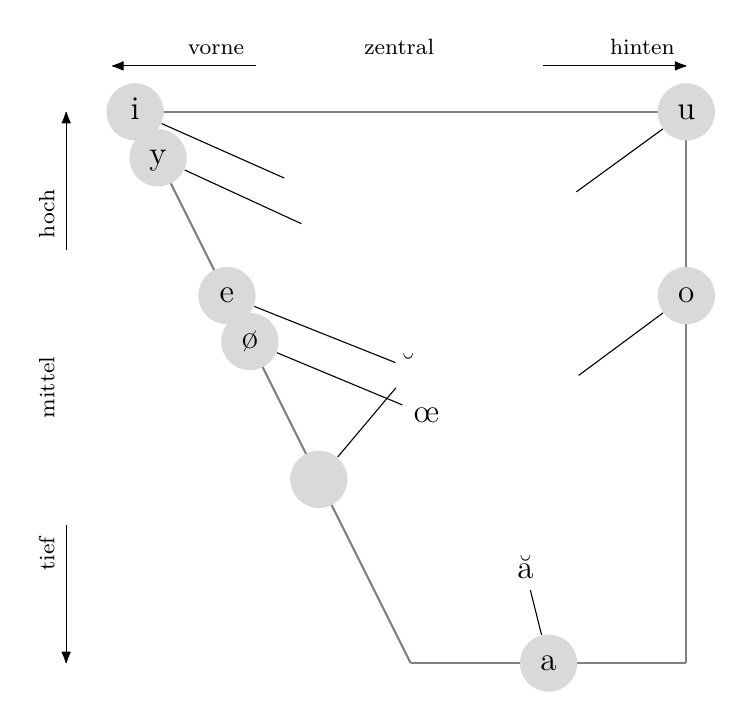
\begin{tikzpicture}[scale=3.5,baseline=default]
    \large
    \tikzset{
    vowel/.style={fill=white, anchor=mid, text depth=0ex, text height=1ex},
    vowelgespannt/.style={circle,fill=gray!30, anchor=mid, text depth=0ex, text height=1ex,minimum size=4ex},
    dot/.style={circle,fill=black,minimum size=0.4ex,inner sep=0pt,outer sep=-1pt},
    }

    \coordinate (hf) at (0,2); % high front
    \coordinate (hb) at (2,2); % high back
    \coordinate (lf) at (1,0); % low front
    \coordinate (lb) at (2,0); % low back
    \def\V(#1,#2){barycentric cs:hf={(3-#1)*(2-#2)},hb={(3-#1)*#2},lf={#1*(2-#2)},lb={#1*#2}}

    % Chart key (vorne -- hinten).
    \draw [{Latex[round]}-] (\V (-.25,0)) -- (\V (-.25,.5))  node [above left] {\footnotesize vorne};
    \draw [-{Latex[round]}] (\V (-.25,1.5)) -- (\V (-.25,2)) node [above left] {\footnotesize hinten};
    \path (\V (-.25,1)) node[above] {\footnotesize zentral};

    % Chart key (hoch--tief).
    \draw [{Latex[round]}-] (\V (0,-.25)) -- +(270:.5cm)  node [above right,rotate=90] (vokaltrapez1) {\footnotesize hoch};
    \draw [{Latex[round]}-] (\V (3,-2.5)) -- +(270:-.5cm) node [above left,rotate=90] (vokaltrapez2) {\footnotesize tief};
    \path (\V (1.5,-1)) node[above,rotate=90] {\footnotesize mittel};

    % Grid.
    \draw [gray,thick] (\V(0,0)) -- (\V(0,2));
    \draw [gray,thick] (\V(3,0)) -- (\V(3,2));
    \draw [gray,thick] (\V(0,0)) -- (\V(3,0));
    \draw [gray,thick] (\V(0,2)) -- (\V(3,2));

    \path (\V(0,0))      node[vowelgespannt] (i)   {i};
    \path (\V(0.25,0))   node[vowelgespannt] (y)   {y};
    \path (\V(0.4,0.5))  node[vowel]         (ii)  {ɪ};
    \path (\V(0.65,0.5)) node[vowel]         (yy)  {ʏ};
    \path (\V(1,0))      node[vowelgespannt] (e)   {e};
    \path (\V(1.25,0))   node[vowelgespannt] (oe)  {ø};
    \path (\V(2,0))      node[vowelgespannt] (ee)  {ɛ};
    \path (\V(1.4,0.7))  node[vowel]         (eee) {ɛ̆};
    \path (\V(1.65,0.7)) node[vowel]         (oee) {œ};
    \path (\V(3,1))      node[vowelgespannt] (a)   {a};
    \path (\V(2.5,1))    node[vowel]         (aa)  {ă};
    \path (\V (1,2))     node[vowelgespannt] (o)   {o};
    \path (\V (1.5,1.4)) node[vowel]         (oo)  {ɔ};
    \path (\V (0,2))     node[vowelgespannt] (u)   {u};
    \path (\V (0.5,1.5)) node[vowel]         (uu)  {ʊ};

    \draw (i)  -- (ii);
    \draw (y)  -- (yy);
    \draw (e)  -- (eee);
    \draw (oe) -- (oee);
    \draw (ee) -- (eee);
    \draw (a)  -- (aa);
    \draw (o)  -- (oo);
    \draw (u)  -- (uu);
  \end{tikzpicture}
  \caption[Phonologisches Vokaltrapez]{Phonologisches Vokaltrapez (Grau für [\textsc{Gespannt}: $+$])}
  \label{fig:gespanntheitbetonungundlaenge019}
  \index{Vokaltrapez}
\end{figure}

Die Vokale in den ersten Silben von \textit{Liebe} [liːbə], \textit{Tüte} [tyːtə], \textit{Wut} [vuːt], \textit{Weg} [veːk], \textit{schön} [ʃøːn], \textit{Käse} [kɛːzə], \textit{rot} [ʁoːt], \textit{rate} [ʁaːtə] gelten also gemäß dieser leicht veränderten Merkmalsmenge als \textit{gespannt}.
In diesen Beispielen sind sie betont und daher lang.
Ungespannte Vokale können betont werden, aber sie werden dadurch nicht lang, \zB \textit{Rinder} [ʁɪndɐ].
Formen wie *[ʁɪːndɐ] sind ausgeschlossen.
Tabelle~\ref{tab:gespanntheitbetonungundlaenge020} gibt einen systematischen Überblick in Form von Beispielen.

\begin{table}[!htbp]
  \centering
  \begin{tabular}{cllp{0.25cm}cll}
    \lsptoprule
    \textbf{gespannt} & \textbf{Beispiel} & \textbf{IPA} & & \textbf{ungespannt} & \textbf{Beispiel} & \textbf{IPA} \\
    \midrule
    i  & \textit{bieten} & biːtən && ɪ & \textit{bitten}  & bɪtən   \\
    y  & \textit{fühlt}  & fyːlt  && ʏ & \textit{füllt}   & fʏlt    \\
    u  & \textit{Mus}    & muːs   && ʊ & \textit{muss}    & mʊs     \\
    e  & \textit{Kehle}  & keːlə  && ɛ & \textit{Kelle}   & kɛlə    \\
    ɛ  & \textit{stähle} & ʃtɛːlə && ɛ & \textit{Ställe}  & ʃtɛlə   \\
    ø & \textit{Höhle}  & høːlə && œ & \textit{Hölle} & hœlə \\
    o  & \textit{Ofen}   & ʔoːfən && ɔ & \textit{offen}   & ʔɔfən   \\
    a  & \textit{Wahn}   & vaːn   && a & \textit{wann}    & van     \\
    \lspbottomrule
  \end{tabular}
  \caption{Gespannte und ungespannte Vokale im Kernwortschatz}
  \label{tab:gespanntheitbetonungundlaenge020}
\end{table}

Was Gespanntheit phonetisch auszeichnet, ist nicht einfach zu bestimmen.
Man kann versuchen, die Kategorie der Gespanntheit mit einer erhöhten Muskelanspannung oder einer Veränderung der Position der Zungenwurzel in Verbindung zu bringen.
Aus Sicht der Phonologie ist der \textit{systematische} Aspekt aber wichtiger als der artikulatorische.
Für die gespannten Vokale gelten gemeinsame Strukturbedingungen, und daher sollte sie die Grammatik idealerweise als eine Klasse von Segmenten auf"|fassen -- genauso wie die stimmhaften und stimmlosen Obstruenten usw.
Mit den Ortsmerkmalen der Vokale und der Lippenrundung alleine könnte man die gespannten (und damit längbaren) Vokale aber nicht von den ungespannten unterscheiden.
Klassen definieren wir über Merkmale und Werte (vgl.\ Abschnitt~\ref{sec:merkmaleundwerte}), und daher ist das neue Merkmal gerechtfertigt.

Weil die halbvorderen und halbhinteren Vokale jetzt durch die Gespanntheit von den vorderen und hinteren unterscheidbar werden, kann ein weiteres Merkmal in seinen möglichen Werten reduziert werden.


\begin{exe}
  \ex \textsc{Lage}: \textit{vorne}, \textit{zentral}, \textit{hinten}
\end{exe}


Je nach Auf"|fassung, was der Kernwortschatz ist, gilt in ihm (auf jeden Fall aber im Erbwortschatz), dass gespannte Vokale immer betont und damit immer lang sind.%
\footnote{Zum Kernwortschatz und Erbwortschatz s.\ Abschnitt~\ref{sec:kernundperipherie}.}
Innerhalb des Kernwortschatzes gibt es damit die in Abbildung~\ref{fig:gespanntheitbetonungundlaenge019} durch Striche verbundenen Paare aus langen gespannten betonten und kurzen ungespannten betonten oder unbetonten Vokalen.
Während die ungespannten betont oder unbetont auftreten können, sind die gespannten immer betont, vgl.\ Satz~\ref{satz:gespanntheitkern}.


\Satz{Gespanntheit im Kernwortschatz}{\label{satz:gespanntheitkern}%
Im Kernwortschatz sind gespannte Vokale immer betont und lang.
Zu jedem gespannten Vokal gibt es einen entsprechenden ungespannten Vokal.
Der ungespannte ist betont oder unbetont, aber immer kurz.}

Im erweiterten Wortschatz, der mehr Wörter mit drei und mehr Silben enthält, gilt die eingangs erwähnte Strukturbedingung, dass bei den gespannten Vokalen die Betonung die Länge kontrolliert.
Beispiele für unbetonte gespannte und damit kurze Vokale sind [i] in (\ref{ex:gespanntheitbetonungundlaenge022}), [e] in (\ref{ex:gespanntheitbetonungundlaenge023}), [u] in (\ref{ex:gespanntheitbetonungundlaenge024}), [o] in (\ref{ex:gespanntheitbetonungundlaenge025}), [ø] in (\ref{ex:gespanntheitbetonungundlaenge026}) und [y] in (\ref{ex:gespanntheitbetonungundlaenge027}).


\begin{exe}
  \ex\label{ex:gespanntheitbetonungundlaenge021}
  \begin{xlist}
    \ex{\label{ex:gespanntheitbetonungundlaenge022} \textit{Idee} [ʔideː]\\
      \textit{Initiative} [ʔinit͡sʝatiːvə]\\
      \textit{inspirieren} [ʔɪnspiʁiːʁən] }
    \ex{\label{ex:gespanntheitbetonungundlaenge023} \textit{Methyl} [metyːl]\\
      \textit{Québec} [kebɛk]\\
      \textit{integriert} [ʔɪntegʁi͡ɐt]\\
      \textit{debattieren} [debatiːʁən] }
    \ex{\label{ex:gespanntheitbetonungundlaenge024} \textit{Utopie} [ʔutopiː]\\
      \textit{Uran} [ʔuʁaːn] }
    \ex{\label{ex:gespanntheitbetonungundlaenge025} \textit{Motiv} [motiːf]\\
      \textit{politisch} [poliːtɪʃ]\\
      \textit{Phonologie} [fonologiː] }
    \ex{\label{ex:gespanntheitbetonungundlaenge026} \textit{Ökonomie} [ʔøkonomiː]\\
      \textit{manövrieren} [manøvʁiːʁən] }
    \ex{\label{ex:gespanntheitbetonungundlaenge027} \textit{Büro} [byʁoː]\\
    \textit{Cuvée} [kyveː] }
  \end{xlist}
\end{exe}


Weil Wörter mit solchen Vokalen im alltäglichen Gebrauch durchaus häufig vorkommen, wird in Satz~\ref{satz:gespannterweitert} nicht von \textit{peripherem Wortschatz}, sondern vorsichtiger vom \textit{erweiterten Wortschatz} gesprochen.


\Satz{Gespanntheit im erweiterten Wortschatz}{\label{satz:gespannterweitert}%
Im erweiterten Wortschatz sind gespannte Vokale lang, wenn sie betont sind, und kurz, wenn sie unbetont sind.
Auch im erweiterten Wortschatz gibt es keine ungespannten langen Vokale.
}

Völlig außerhalb dieses Systems stehen Schwa und [ɐ] gemäß Satz~\ref{satz:schwabetont}.

\Satz{Schwa}{\label{satz:schwabetont}%
Schwa und [ɐ] sind immer kurz und nie betont.
}

Damit müssen die zugrundeliegenden Formen genau wie bei der Endrand"=Desonorisierung gemäß der neu eingeführten Strukturbedingungen angepasst werden.
Länge muss nicht mehr zugrundeliegend spezifiziert werden, und man erhält Beispiele wie in (\ref{ex:gespanntheitbetonungundlaenge028}).

\begin{exe}
  \ex\label{ex:gespanntheitbetonungundlaenge028} \begin{xlist}
    \ex /veg/ \phopro [veːk]
    \ex /hølə/ \phopro [høːlə]
    \ex /ofən/ \phopro [ʔoːfən]
  \end{xlist}
\end{exe}

\subsection{Verteilung von [ç] und [χ]}
\label{sec:verteilungvonund}

Die sogenannten \textit{ich}- und \textit{ach}-Segmente sind komplementär verteilt.
Es gibt kein Wort, in dem sie einen lexikalischen Unterschied markieren.
Einige Beispielwörter, in denen [ç] und [χ] vorkommen, illustrieren diese Verteilungen in (\ref{ex:verteilungvonund029}).

\begin{exe}
  \ex\label{ex:verteilungvonund029}
  \begin{xlist}
    \ex{\label{ex:verteilungvonund030} krieche, schlich, Bücher, Küche, Recht, Köche}
    \ex{\label{ex:verteilungvonund031} Tuch, Geruch, hoch, Koch, Schmach, Bach}
  \end{xlist}
\end{exe}

Ausschlaggebend für das Vorkommen von [ç] und [χ] ist der unmittelbar vorangehende Kontext.
Nach /i/, /ɪ/, /y/, /ʏ/, /e/, /ɛ/, /ɛ̆/, /ø/, /œ/ kommt [ç] vor, nach /u/, /ʊ/, /o/, /ɔ/, /a/ und /ă/ hingegen [χ].
Nach Schwa kommt keins der beiden Segmente vor.
Ein Blick auf das phonologische Vokaltrapez in Abbildung~\ref{fig:gespanntheitbetonungundlaenge019} zeigt sofort, was der relevante Merkmalsunterschied zwischen den beiden Gruppen von Vokalen ist.
Nach Vokalen, die [\textsc{Lage}: \textit{vorne}] sind, steht [ç].
Nach allen anderen Vokalen steht hingegen [χ].
Es handelt sich hier um eine Angleichung des Artikulationsorts des Frikativs an den hinterer Vokale, eine sogenannte \textit{Assimilation}.\index{Assimilation}

Es muss jetzt nur noch entschieden werden, wie die zugrundeliegende Form in diesem Fall aussieht.
Aufschlussreich ist hier die Betrachtung von Wörtern wie \textit{Milch} /mɪlç/, \textit{Storch} /ʃtɔʁç/ oder \textit{Röckchen} /ʁœkçən/, in denen [ç], aber niemals [χ] nach einem Konsonanten vorkommt.
Dies ist generell der Fall, und es ist deswegen günstiger, anzunehmen, dass /ç/ zugrundeliegt und [χ] das phonetische Resultat einer Assimilation ist.
Das heißt, dass [χ] kein zugrundeliegendes Segment ist und nicht in /~/ gehört.
Mit der entsprechenden Strukturbedingung aus Satz~\ref{satz:cassimilation} ergeben sich die Beispiele wie in (\ref{ex:verteilungvonund032}).

\Satz{/ç/-Assimilation}{\label{satz:cassimilation}%
[ç] kann nicht nach Vokalen stehen, die nicht [\textsc{Lage}: \textit{vorne}] sind.
Zugrundeliegendes /ç/ wird daher nach zentralen und hinteren Vokalen weiter hinten artikuliert, nämlich als [χ].}

\begin{exe}
  \ex\label{ex:verteilungvonund032}
  \begin{xlist}
    \ex{/ɪç/ \phopro [ʔɪç]}
    \ex{/ăç/ \phopro [ʔaχ]}
  \end{xlist}
\end{exe}

\subsection{/ʁ/-Vokalisierungen}
\label{sec:vokalisierungen}

In Abschnitt~\ref{sec:orthographischesr} wurden phonetische Korrelate von geschriebenem \textit{r} besprochen.
Die Schrift ist hier besonders systematisch, denn orthographisches \textit{r} entspricht immer einem zugrundeliegenden /ʁ/ (s.\ auch Abschnitt~\ref{sec:buchstabenundphonologischesegmente}).
In (\ref{ex:vokalisierungen033}) sind Beispiele zusammengestellt (inklusive der Silbengrenzen in Form von Punkten), die dies illustrieren.

\begin{exe}
  \ex\label{ex:vokalisierungen033}
  \begin{xlist}
    \ex{kleiner [kla͡ɛ.nɐ], kleinere [kla͡ɛ.nə.ʁə]}
    \ex{Bär [bɛ͡ɐ], Bären [bɛː.ʁən]}
    \ex{knarr [kna͡ə], knarre [kna.ʁə]}
  \end{xlist}
\end{exe}

Wenn ein zugrundeliegendes /ʁ/ am Silbenanfang steht, wird es als Konsonant [ʁ] realisiert.
Demgegenüber findet am Silbenende immer eine Vokalisierung von /ʁ/ statt.
Nach gespannten Vokalen wird /ʁ/ zu [ɐ], nach ungespannten zu [ə].
Nach (stets unbetontem) Schwa wird /ʁ/ gar nicht realisiert, und Schwa wird zu [ɐ].
Diese Vorgänge formal genau aufzuschreiben, würde den hier gegebenen Rahmen sprengen.
Aus Sicht der Phonologie sind die Unterschiede zwischen [ə] und [ɐ] auch nicht erheblich, denn diese Segmente stellen nur minimal unterschiedliche Färbungen des Schwa-Segments dar.
Beispiele folgen in (\ref{ex:vokalisierungen034}).

\begin{exe}
  \ex \label{ex:vokalisierungen034}
  \begin{xlist}
    \ex /kla͡ɛnəʁ/ \phopro [kla͡ɛ.nɐ]
    \ex /tiʁ/ \phopro [ti͡ɐ]
    \ex /bɪʁkə/ \phopro [bɪ͡ə.kə]
  \end{xlist}
\end{exe}

Die entsprechende Strukturbedingung und ihre Effekte werden in Satz~\ref{satz:rvokalisierung} beschrieben.

\Satz{/ʁ/-Vokalisierung}{\label{satz:rvokalisierung}%
Zugrundeliegendes /ʁ/ kann nicht am Silbenende stehen.
Es wird in dieser Position als Schwa-Segment im sekundären Diphthong realisiert.
Nach gespanntem Vokal folgt [ɐ], nach ungespanntem folgt [ə].
Schwa und /ʁ/ werden zusammen durch [ɐ] substituiert.
}

\Zusammenfassung{%
In der Phonologie ist der Status der Segmente im Gesamtsystem relevant.
Dabei werden vor allem ihre Verteilung und ihre Merkmale betrachtet.
Wenn man alle Formen eines Worts berücksichtigt, kann man umgebungsabhängige bzw.\ positionsabhängige Änderungen von Merkmalswerten beobachten.
Um solche Phänomene adäquat zu beschreiben, nimmt man abstraktere zugrundeliegende Formen an, die an phonologische Strukturbedingungen wie die Endrand-Desonorisierung angepasst werden.
}


\include{chapters/07Silben}
\include{chapters/07Silben}
\include{chapters/08Staemme}
\include{chapters/09Wortbildung}
\include{chapters/10Nomina}
\include{chapters/11Verben}
\include{chapters/12Konstituenten}
\include{chapters/13Phrasen}
\include{chapters/14Saetze}
\chapter{Passiv}
\label{sec:Passiv}

\section{Semantische Rollen}
\label{sec:semantischerollen}

\subsection{Verbsemantik und Rollen}
\label{sec:verbsemantikundrollen}

In den folgenden Abschnitten wird es immer wieder nötig sein, auf die Bedeutung von Verben bezugzunehmen.
Es wurde zwar in Abschnitt~\ref{sec:kasus} abgelehnt, Kasus an sich eine Bedeutung zuzusprechen (besonders für den Nominativ und den Akkusativ, eingeschränkt für den Dativ und Genitiv), aber bestimmte Muster von Kasusverteilungen bei verschiedenen Typen von Verben lassen sich besser verstehen, wenn man ein System zugrundelegt, nach dem die Verbbedeutung die Wahl verschiedener Kasus beeinflusst.
Es ändert sich also nichts daran, dass Kasus an sich keine Bedeutung hat, sondern wir systematisieren nur das Verhältnis von Verbbedeutung und Kasusmustern.

Dazu wird ein System von sogenannten \textit{semantischen Rollen} zugrundegelegt, die manchmal auch \textit{thematische Rollen} oder \textit{Theta-Rollen} bzw.\ $\theta$\textit{-Rollen} genannt werden.
Man kann Verben so verstehen, dass sie ein Ereignis (\zB \textit{kaufen}) oder einen Zustand (\zB \textit{liegen}) bezeichnen, wobei für Ereignisse und Zustände mit einem Sammelbegriff von \textit{Situationen} gesprochen wird.
In einer von einem Verb beschriebenen Situation gibt es typischerweise beteiligte Gegenstände i.\,w.\,S.\ (wie das Gekaufte bei \textit{kaufen}).
Diese Gegenstände spielen eine typische \textit{Rolle} in den Situationen, wie sie durch das Verb beschrieben werden.
Diese Rolle kann man semantisch spezifizieren.
Der Käufer in einer \textit{kaufen}-Situation handelt \zB aktiv und willentlich, das Gekaufte handelt nicht auf diese Weise, aber es wechselt den Besitzer im Rahmen der Situation.
Allgemein soll Definition~\ref{def:semrolle} gelten.

\Definition{Semantische Rolle}{\label{def:semrolle}%
Eine\textit{ semantische Rolle} ist die charakteristische Rolle, die ein beteiligter Gegenstand (Mitspieler) in einer von einem Verb beschriebenen Situation spielt.
Mitspieler können konkrete oder abstrakte Gegenstände (einschließlich Lebewesen und Menschen), andere Situationen usw.\ sein.
\index{Rolle}
\index{Mitspieler}
}

Typischerweise abstrahiert man von für einzelne Verben spezifischen Rollen (wie \textit{Käufer} und \textit{Gekauftes}) und entwickelt ein reduziertes Inventar von semantischen Rollen, die mit grammatischen Phänomenen in Verbindung stehen.
Wie viele und welche dies konkret sind, wird unterschiedlich gesehen.
In fast allen Ansätzen gibt es die Rollen \textit{Agens} (den \textit{Handelnden}), \textit{Patiens} (den \textit{Erdulder}) und \textit{Experiencer} (den bewusst \textit{Erlebenden}).
Für die hier besprochenen Phänomene reicht es, zwischen Agens, Experiencer und allen anderen Rollen zu unterscheiden.

Was ein Agens ist, haben wir im Grunde schon illustriert.
Die Sätze in (\ref{ex:verbsemantikundrollen001}) zeigen die hier vertretene Dreiteilung.

\begin{exe}
  \ex\label{ex:verbsemantikundrollen001}
  \begin{xlist}
    \ex{\label{ex:verbsemantikundrollen002} Michelle kauft einen Rottweiler.}
    \ex{\label{ex:verbsemantikundrollen003} Der Rottweiler schläft.}
    \ex{\label{ex:verbsemantikundrollen004} Der Rottweiler erfreut Marina.}
  \end{xlist}
\end{exe}

In der Bedeutung von (\ref{ex:verbsemantikundrollen002}) gibt es eine \textit{kaufen}-Situation.
Dabei ist Michelle der willentlich handelnde Mitspieler, also ein Agens.
Der Rottweiler handelt nicht, und es wird kein besonderer psychischer Zustand in ihm ausgelöst, womit er weder ein Agens noch ein Experiencer ist.
Hierbei ist eine wichtige Einschränkung zu beachten: Es wird sicherlich irgendeinen psychischen Zustand beim Hund und bei Michelle auslösen, an dem \textit{kaufen}-Ereignis beteiligt zu sein (\zB Freude bei Michelle und anfängliche Skepsis bei dem Rottweiler), aber die Bedeutung von \textit{kaufen} enthält keine spezifische Beschreibung solcher Zustände bei den Mitspielern.
Es geht bei der Rollenvergabe also nur um den Beitrag der Semantik des konkreten Verbs.
Was wir sonst noch bei der Interpretation eines Satzes wissen oder inferieren können, hat nichts mit den semantischen Rollen zu tun.

Die Mitspieler einer \textit{schlafen}-Situation wie in Satz (\ref{ex:verbsemantikundrollen003}) unterscheiden sich deutlich von denen einer \textit{kaufen}-Situation.
Es gibt nur ein beteiligtes Objekt, das weder Agens noch Patiens ist, hier der Rottweiler.
In (\ref{ex:verbsemantikundrollen004}) ist Marina ein Experiencer, denn das Verb \textit{erfreuen} bezeichnet Situationen, in denen ein ganz spezifischer psychischer Zustand (der der Freude) ausgelöst wird.
Ob der Rottweiler hier ein Agens ist, ist schwieriger zu beurteilen, da nicht ganz klar ist, ob er durch seine schiere Anwesenheit oder durch sein Verhalten erfreut.
Selbst wenn es sein Verhalten wäre, wäre fraglich, ob man bei einem Hund von \textit{willentlichem Handeln} sprechen könnte.
In Abschnitt~\ref{sec:passiv} wird sich eine Lösung für dieses Problem abzeichnen, die gleichzeitig neue Probleme mit sich bringt (vgl.\ Vertiefung \ref{vert:agensprobleme} auf Seite~\pageref{vert:agensprobleme}).
Die Definitionen~\ref{def:agens} und~\ref{def:experiencer} fassen das bisher Gesagte zusammen.

\Definition{Agens}{\label{def:agens}%
Das \textit{Agens} ist der willentlich handelnde Mitspieler in einer von einem Verb bezeichneten Situation.
\index{Agens}
}

\Definition{Experiencer}{\label{def:experiencer}%
Ein \textit{Experiencer} ist ein Mitspieler in einer von einem Verb bezeichneten Situation, bei dem ein spezifischer psychischer Zustand ausgelöst wird.
\index{Experiencer}
}

Es ergeben sich nun bestimmte Muster von semantischen Rollen bei Verben, die wir als Liste angeben können.
Wir bezeichnen hier dabei alle anderen Rollen außer Agens und Experiencer mit dem Platzhalter \textit{Rx} (für \textit{Rolle x} im Sinn von \textit{beliebige andere Rolle}), weil ihre Differenzierung für unsere Zwecke nicht erforderlich ist.
In ausführlicheren Analysen stünde statt \textit{Rx} eine größere Anzahl konkreter anderer Rollen.
Damit hat \zB \textit{kaufen} ein Rollenmuster \Rollen{Agens, Rx}.
Für die bisher besprochenen Verben ergibt sich insgesamt (\ref{ex:verbsemantikundrollen005}).

\begin{exe}
  \ex\label{ex:verbsemantikundrollen005}
  \begin{xlist}
    \ex{\label{ex:verbsemantikundrollen006}\textit{kaufen}: \Rollen{Agens,~Rx} }
    \ex{\label{ex:verbsemantikundrollen007}\textit{schlafen}: \Rollen{Rx} }
    \ex{\label{ex:verbsemantikundrollen008}\textit{erfreuen}: \Rollen{Rx,~Experiencer}\\
      oder vielleicht \Rollen{Agens,~Experiencer} }
  \end{xlist}
\end{exe}

Die Rollenverteilungen sind bei allen Vorkommen dieser Verben dieselben.
Das Rollenmuster ist also eine lexikalische Eigenschaft der Verben, und man kann daher auch von \textit{Verbtypen} sprechen, die durch Rollenmuster definiert werden.
Ein Verb wie \textit{erschrecken} hat dann denselben Typ wie \textit{erfreuen}.
\textit{anheben} hat denselben Typ wie \textit{kaufen}, usw.
Es gibt aber eben kein \textit{kaufen}-Ereignis, bei dem das Gekaufte willentlich handelt, Rollen- oder Sprachspiele ausgenommen.%
\footnote{Solche Spiele leben gerade davon, dass die besprochenen Regularitäten auf kreative Weise gebrochen werden.}
Ein üblicherweise angenommenes Prinzip, das sich zum Beispiel in Abschnitt~\ref{sec:artenvonesimnominativ} als sehr nützlich erweisen wird, besagt dabei, dass ein Verb jede Rolle nur einmal vergeben kann, vgl.\ Satz~\ref{satz:thetaprinz}.

\Satz{Prinzip der Rollenzuweisung}{\label{satz:thetaprinz}%
Jedes Verb kann eine von ihm zu vergebende Rolle nur einmal (also nur an eine Konstituente) vergeben.
Nicht alle Rollen müssen in jedem Satz vergeben werden (\zB bei fakultativen Ergänzungen).
\index{Rolle}
}

Bisher wurde nur von Verben als Rollen-Zuweiser gesprochen.
Das ist ein bisschen zu eng gefasst, da auch lexikalisierte Gefüge wie \textit{zu denken geben}, Adjektive wie \textit{wütend} und Substantive wie \textit{Aufteilung} Rollen vergeben.
Obwohl der Prädikatsbegriff nicht leicht präzise zu definieren ist (s.\ Abschnitt~\ref{sec:praedikateundpraedikativekonstituenten}), kann man allgemeiner davon sprechen, dass Rollen von Prädikaten zugewiesen werden.
Unabhängig davon muss man annehmen, dass die Präpositionen in PP-Angaben den regierten NPs eine Rolle zuweisen, und dass der Kasus freier NP-Angaben direkter Ausdruck einer freien Rolle ist.\index{Angabe!präpositional}
In (\ref{ex:verbsemantikundrollen009}) wird \textit{dem Tisch} die Rolle (der Ort der Situation) von der Präposition \textit{unter} zugewiesen.
Die lokale PP \textit{unter dem Tisch} bringt ihre Rolle sozusagen ganz unabhängig vom Verb mit.

\begin{exe}
  \ex{\label{ex:verbsemantikundrollen009} Der Rottweiler schläft [unter dem Tisch].}
\end{exe}

\subsection{Semantische Rollen und Valenz}
\label{sec:semantischerollenundvalenz}

\index{Valenz}\index{Rolle}

Interessant ist für die Grammatik (wie soeben angedeutet) die Verknüpfung der von einem Verb zugewiesenen semantischen Rollen mit seiner Valenz.
In Abschnitt~\ref{sec:valenz} haben wir uns nicht ganz erfolgreich bemüht, Valenz ohne Bezug zur Semantik zu definieren.
Valenz ist laut Definition~\ref{def:ergang} und Definition~\ref{def:valenz} die Liste der von einer Einheit subklassenspezifisch lizenzierten anderen Einheiten.
Man kann auch versuchen, den Unterschied zwischen Ergänzungen und Angaben stärker an die Rollensemantik eines Verbs zu knüpfen.
Im Vorgriff auf die Abschnitte~\ref{sec:dativeundindirekteobjekte} und~\ref{sec:ppergaenzungenundppangaben} nehmen wir die Beispiele in (\ref{ex:semantischerollenundvalenz010}) und (\ref{ex:semantischerollenundvalenz013}).

\begin{exe}
  \ex\label{ex:semantischerollenundvalenz010}
  \begin{xlist}
    \ex{\label{ex:semantischerollenundvalenz011} Michelle schenkt [ihrer Freundin] die Hundeleine.}
    \ex{\label{ex:semantischerollenundvalenz012} Michelle fährt [ihrer Freundin] zu schnell.}
  \end{xlist}
  \ex\label{ex:semantischerollenundvalenz013}
  \begin{xlist}
    \ex{\label{ex:semantischerollenundvalenz014} Michelle denkt [an Marina].}
    \ex{\label{ex:semantischerollenundvalenz015} Michelle rennt [an die Tür].}
  \end{xlist}
\end{exe}

Beim Dativ zu \textit{schenken} in (\ref{ex:semantischerollenundvalenz011}) und bei der \textit{an}-PP zu \textit{denken} in (\ref{ex:semantischerollenundvalenz014}) würde man von Ergänzungen sprechen.\index{Ergänzung}\index{Angabe}
In (\ref{ex:semantischerollenundvalenz012}) und (\ref{ex:semantischerollenundvalenz015}) wird der Dativ bzw.\ die \textit{an}-PP aber eher als Angabe analysiert.
Bemerkenswert ist, dass der Unterschied zwischen Ergänzungen und Angaben hier mit einem Unterschied in der Rollenzuweisung einhergeht.
Die Rolle des Geschenk-Empfängers bei \textit{schenken}-Situationen, die immer dem Dativ-Mitspieler zugewiesen wird, wird durch das Verb eindeutig festgelegt.
Dasselbe gilt für den \textit{an}-PP-Mitspieler bei \textit{denken}-Situationen wie in (\ref{ex:semantischerollenundvalenz014}).
Der Dativ in (\ref{ex:semantischerollenundvalenz012}) hingegen bezeichnet jemanden, der die Situation einschätzt.\index{Dativ!frei}
Die Rolle des Einschätzers wird aber sicherlich nicht von \textit{fahren} zugewiesen, denn es ist nicht Teil der Bedeutung von \textit{fahren}, dass an \textit{fahren}-Situationen ein Mitspieler beteiligt ist, der die Geschwindigkeit beurteilt.
Genauso ist die Rolle des \textit{an}-PP-Mitspielers in (\ref{ex:semantischerollenundvalenz015}) nicht wie bei \textit{denken} durch \textit{rennen} festgelegt.
Die nicht im Valenzrahmen des Verbs verankerten Angaben haben also eine vom Verb unabhängige Rolle, was besonders für PPs typisch ist, aber eben auch bei nicht regierten Kasus auftritt.
Passend dazu verliert die \textit{an}-PP bei \textit{denken} ihre für die Präposition \textit{an} spezifische Rolle (Zielort), da sie eine Ergänzung ist und das Verb die Rollenzuweisung alleine steuert.
In weiteren Abschnitten werden diese Verhältnisse immer wieder aufs Tapet kommen.
Eine zweifelsfreie Trennung von Ergänzungen und Angaben wird damit zwar besser angenähert, bleibt praktisch aber schwierig.
In Abschnitt~\ref{sec:artenvonesimnominativ} werden wir überdies sehen, dass das Pronomen \textit{es} bei Verben wie \textit{regnen} als Ergänzung auftritt, ohne dass ihm eine Rolle zugewiesen wird.

\Zusammenfassung{%
Semantische Rollen klassifizieren die Mitspieler an einer durch ein Verb beschriebenen Situation, \zB nach Agentivität, aber es gibt keine vom Verbtyp unabhängige Beziehung zwischen Rollen und Kasus.
}

\section{Passiv}
\label{sec:passiv}

\subsection{\textit{werden}-Passiv und Verbtypen}
\label{sec:werdenpassivundverbtypen}

\index{Passiv!werden--}

Über das \textit{werden}-Passiv (das oft auch nur als das \textit{Passiv} schlechthin oder das \textit{Vorgangspassiv} bezeichnet wird) wurde in diesem Buch schon wiederkehrend gesprochen, \zB in Abschnitt~\ref{sec:genusverbi} oder im Kontext der Subjekts- und Objektsgenitive in Abschnitt~\ref{sec:rektionundvalenzindernp}.
Hier wird die Bildung noch einmal zusammengefasst und vertieft, vor allem indem die Unterklassifikation der Vollverben genauer herausgearbeitet wird.
Ausgangspunkt sind die Paare von Aktiv- und Passivsätzen in (\ref{ex:werdenpassivundverbtypen110}) bis (\ref{ex:werdenpassivundverbtypen125}).

\newcommand{\Lab}[1]{\ensuremath{_{\mathrm{#1}}}}
\begin{exe}
  \ex\label{ex:werdenpassivundverbtypen110}
  \begin{xlist}
    \ex[ ]{\label{ex:werdenpassivundverbtypen111} Johan wäscht den Wagen.}
    \ex[ ]{\label{ex:werdenpassivundverbtypen112} Der Wagen wird (von Johan) gewaschen.}
  \end{xlist}
  \ex\label{ex:werdenpassivundverbtypen113}
  \begin{xlist}
    \ex[ ]{\label{ex:werdenpassivundverbtypen114} Alma schenkt dem Schlossherrn den Roman.}
    \ex[ ]{\label{ex:werdenpassivundverbtypen115} Der Roman wird dem Schlossherrn (von Alma) geschenkt.}
  \end{xlist}
  \ex\label{ex:werdenpassivundverbtypen116}
  \begin{xlist}
    \ex[ ]{\label{ex:werdenpassivundverbtypen117} Johan bringt den Brief zur Post.}
    \ex[ ]{\label{ex:werdenpassivundverbtypen118} Der Brief wird (von Johan) zur Post gebracht.}
  \end{xlist}
  \ex\label{ex:werdenpassivundverbtypen119}
  \begin{xlist}
    \ex[ ]{\label{ex:werdenpassivundverbtypen120} Der Maler dankt den Fremden.}
    \ex[ ]{\label{ex:werdenpassivundverbtypen121} Den Fremden wird (vom Maler) gedankt.}
  \end{xlist}
  \ex\label{ex:werdenpassivundverbtypen122}
  \begin{xlist}
    \ex[ ]{\label{ex:werdenpassivundverbtypen123} Johan arbeitet hier immer montags.}
    \ex[ ]{\label{ex:werdenpassivundverbtypen124} Montags wird hier (von Johan) immer gearbeitet.}
  \end{xlist}
  \ex\label{ex:werdenpassivundverbtypen125}
  \begin{xlist}
    \ex[ ]{\label{ex:werdenpassivundverbtypen126} Der Ball platzt bei zu hohem Druck.}
    \ex[*]{\label{ex:werdenpassivundverbtypen127} Bei zu hohem Druck wird (vom Ball) geplatzt.}
  \end{xlist}
  \ex\label{ex:werdenpassivundverbtypen128}
  \begin{xlist}
    \ex[ ]{\label{ex:werdenpassivundverbtypen129} Der Rottweiler fällt Michelle auf.}
    \ex[*]{\label{ex:werdenpassivundverbtypen130} Michelle wird (von dem Rottweiler) aufgefallen.}
  \end{xlist}
\end{exe}

\index{Verb!transitiv}
\index{Passiv!unpersönlich}
\index{Valenz}

Die (b)-Sätze in (\ref{ex:werdenpassivundverbtypen110})--(\ref{ex:werdenpassivundverbtypen128}) sind jeweils Passivbildungen zu den Aktivsätzen in (a).
Außer dass das Vollverb im Partizip auftritt (\textit{wäscht}--\textit{gewaschen} usw.) und das Hilfsverb \textit{werden} als finites Verb hinzukommt, ergibt sich ein relativ klares Muster bezüglich der Valenzänderungen vom Aktivverb zum zugehörigen Passivverb.
Wie schon mehrfach erwähnt, wird der Nominativ des Aktivs entfernt, kann aber optional als PP mit \textit{von} formuliert werden.
Diese PP kann man als fakultative Ergänzung oder als Angabe analysieren.
Wir sagen tendentiell, dass es eine fakultative Ergänzung ist, weil sie spezifisch für eine formal klar abgrenzbare Klasse von Verben ist, nämlich die passivierten Verben.

Wenn das Verb im Aktiv einen Akkusativ hat (wie \textit{waschen}, \textit{schenken}, \textit{bringen}), wird dieser zum Nominativ des Passivs.
Falls das aber nicht so ist, ergeben sich im Passiv Sätze ohne Nominativ und damit ohne Subjekt wie (\ref{ex:werdenpassivundverbtypen121}), (\ref{ex:werdenpassivundverbtypen124}), die manchmal auch \textit{unpersönliches Passiv} genannt werden.
Alle anderen Ergänzungen bleiben unverändert, also hier der Dativ von \textit{schenken} (\textit{dem Schlossherrn}), die PP-Ergänzung bei \textit{bringen} (\textit{zur Post}) und der Dativ bei \textit{danken} (\textit{den Fremden}).
Diesen Valenzunterschied zwischen Aktiv und Passiv sehen wir bei allen Verben außer \textit{platzen} (\ref{ex:werdenpassivundverbtypen125}) und \textit{auf"|fallen} (\ref{ex:werdenpassivundverbtypen128}), die als einzige Verben in den Beispielen überhaupt keine Passivbildung zulassen.
Im Gegensatz zur naiven Aussage, nur transitive Verben (also solche mit einer Nominativ- und einer Akkusativ-Ergänzung) könnten ein Passiv bilden, können also \zB auch Verben, die nur einen Nominativ und einen Dativ regieren (\textit{danken}) passiviert werden.
Sogar bestimmte intransitive Verben wie \textit{arbeiten} können passiviert werden, andere allerdings nicht (\textit{platzen}).
Auch Verben mit PP-Ergänzungen (\textit{glauben an}) oder Genitiv (\textit{gedenken}), die hier aus Platzgründen weggelassen wurden, sind passivierbar.
Das \textit{werden}-Passiv betrifft also vor allem den Nominativ und nur nachrangig den Akkusativ.

Es bleibt die Frage, warum Verben wie \textit{platzen} und \textit{auf"|fallen} nicht passivierbar sind, obwohl sie dasselbe Valenzmuster haben wie \textit{arbeiten} bzw.\ \textit{danken}.
Die Antwort lässt sich auf die Rollenverteilung bei diesen Verben zurückführen.
Bei passivierbaren Verben wird dem Nominativ des Aktivs prototypisch vom Verb eine Agens"=Rolle zugewiesen.\index{Agens}
In \textit{platzen}- und \textit{auf"|fallen}-Situationen gibt es aber keinen willentlich Handelnden, die entsprechenden Situationen sind vielmehr unwillkürliche Widerfahrnisse.
Es gilt also Satz~\ref{satz:werdenpass}, der im Grunde informell eine Lexikonregel beschreibt (vgl.\ Abschnitt~\ref{sec:lexikonregeln}).
Eine solche Lexikonregel würde dabei nicht nur Verben mit veränderter Valenzstruktur erzeugen, sondern wäre auch für morphologische Wortformenbildung zuständig.


\index{Lexikon!Regel}

\Satz{\textit{werden}-Passiv}{\label{satz:werdenpass}%
Das \textit{werden}"=Passiv kann prototypisch von Verben mit einem agentiven Nominativ durch Veränderungen der Valenz des Verbs (\zB durch eine Lexikonregel) gebildet werden.
Die Nominativ-Ergänzung des Aktivs wird zu einer fakultativen \textit{von}"=PP des Passivs.
Falls der Aktiv einen Akkusativ hat, wird er zum Nominativ des Passivs.
\index{Passiv!als Valenzänderung}
\index{Passiv!werden--}
}

\index{Verb!unergativ}
\index{Verb!unakkusativ}
\index{Verb!intransitiv}

Es gibt nach dieser Darstellung zwei Arten von sogenannten intransitiven Verben, nämlich solche, die einen agentiven Nominativ haben (sogenannte \textit{unergative} Verben) wie \textit{arbeiten} und solche, die einen nicht-agentiven Nominativ haben (sogenannte \textit{unakkusative} Verben) wie \textit{platzen}.%
\footnote{Statt von \textit{unergativen} und \textit{unakkusativen Verben} sprechen manche von \textit{unergativischen} und \textit{unakkusativischen Verben}.}
Als Test bietet sich die Passivierbarkeit an (nur unergative intransitive Verben sind passivierbar).
Damit ergibt sich eine Klassifikation für die hier besprochenen Verbtypen wie in Tabelle~\ref{tab:werdenpassivundverbtypen131}, wobei agentive Nominative als Nom\_Ag gekennzeichnet sind.
Dass Satz~\ref{satz:werdenpass} das Wort \textit{prototypisch} enthält, liegt daran, dass die Generalisierung nur ungefähr zutrifft.
Vertiefung~\ref{vert:agensprobleme} bespricht eins der Probleme.

\begin{table}[!htbp]
    \begin{tabular}{lllll}
      \lsptoprule
      \textbf{Valenz} & \textbf{Passiv} & \textbf{Name} & \textbf{Beispiel} \\
      \midrule
      Nom\_Ag & ja & Unergative & \textit{arbeiten} \\
      Nom & nein & Unakkusative & \textit{platzen} \\
      Nom\_Ag, Akk & ja & Transitive & \textit{waschen} \\
      Nom\_Ag, Dat & ja & unergative Dativverben & \textit{danken} \\
      Nom, Dat & nein & unakkusative Dativverben & \textit{auf"|fallen} \\
      Nom\_Ag, Dat, Akk & ja & Ditransitive & \textit{geben} \\
      \lspbottomrule
    \end{tabular}
  \caption{Typen von Vollverben nach Valenz und Agentivität}
  \label{tab:werdenpassivundverbtypen131}
\end{table}


\begin{Vertiefung}{Probleme der Agens-Definition}

  \label{vert:agensprobleme}
  \index{Agens}

\noindent Die hier verwendeten Definitionen für das Agens und für das \textit{werden}-Passiv erlauben es, die Passivierbarkeit eines Verbs als Zeichen dafür zu interpretieren, dass das Verb ein agentives Subjekt hat.
Wir können damit versuchen, zu entscheiden, ob das Subjekt bei \textit{ängstigen} tatsächlich agentiv ist, s.\ (\ref{ex:werdenpassivundverbtypen132}).
Gleichzeitig tritt aber ein neues Problem auf, das in (\ref{ex:werdenpassivundverbtypen135}) zu beobachten ist.

\begin{exe}
  \ex\label{ex:werdenpassivundverbtypen132}
  \begin{xlist}
    \ex[ ]{\label{ex:werdenpassivundverbtypen133} Der Rottweiler ängstigt Marina.}
    \ex[*]{\label{ex:werdenpassivundverbtypen134} Marina wird von dem Rottweiler geängstigt.}
  \end{xlist}
  \ex\label{ex:werdenpassivundverbtypen135}
  \begin{xlist}
    \ex[ ]{\label{ex:werdenpassivundverbtypen136} Eine Wolke überholt den Pteranodon.}
    \ex[ ]{\label{ex:werdenpassivundverbtypen137} Der Pteranodon wird von einer Wolke überholt.}
  \end{xlist}
\end{exe}

(\ref{ex:werdenpassivundverbtypen134}) legt nahe, dass man das Subjekt von \textit{ängstigen} eher nicht als Agens klassifizieren sollte, weil das Verb schlecht passivierbar ist.
Allerdings lässt sich \textit{überholen} mit dem Subjekt \textit{eine Wolke}, das ganz sicher kein willentlich handelndes Wesen bezeichnet, passivieren.
Satz (\ref{ex:werdenpassivundverbtypen137}) ist einwandfrei grammatisch.
Eine Lösung für dieses Problem zu erarbeiten, würde den hier gegebenen Rahmen sprengen.
Sie kann nur darin liegen, den Begriff des Agens nicht über eine einzige Eigenschaft \textit{willentlich handelnd} kategorisch zu definieren.
Es wird dringend \citet{Dowty1991} zur Lektüre empfohlen.

\end{Vertiefung}

\subsection{\textit{bekommen}-Passiv}
\label{sec:bekommenpassiv}

Das \textit{werden}-Passiv ist nicht die Passivbildung schlechthin im Deutschen.
Verschiedene andere Bildungen sind im Prinzip auch Passive, unter anderem das \textit{bekommen}-Passiv in (\ref{ex:bekommenpassiv138}).

\begin{exe}
  \ex\label{ex:bekommenpassiv138}
  \begin{xlist}
    \ex[ ]{\label{ex:bekommenpassiv139} Mein Kollege bekommt den Wagen (von Johan) gewaschen.}
    \ex[ ]{\label{ex:bekommenpassiv140} Der Schlossherr bekommt den Roman (von Alma) geschenkt.}
    \ex[ ]{\label{ex:bekommenpassiv141} Mein Kollege bekommt den Brief (von Johan) zur Post gebracht.}
    \ex[ ]{\label{ex:bekommenpassiv142} Die Fremden bekommen (von dem Maler) gedankt.}
    \ex[?]{\label{ex:bekommenpassiv143} Mein Kollege bekommt hier immer montags (von Johan) gearbeitet.}
    \ex[*]{\label{ex:bekommenpassiv144} Mein Kollege bekommt bei zu hohem Druck (von dem Ball) geplatzt.}
    \ex[*]{\label{ex:bekommenpassiv145} Michelle bekommt (von dem Rottweiler) aufgefallen.}
  \end{xlist}
\end{exe}

Hier treten mit kleinen Veränderungen die in Abschnitt~\ref{sec:werdenpassivundverbtypen} als Beispiele verwendeten Verben in einer Konstruktion mit dem Verb \textit{bekommen} im Partizip auf.
Wie beim \textit{werden}-Passiv wird der agentive Nominativ des Aktivs zur fakultativen \textit{von}-PP.
Dass \textit{platzen} (\ref{ex:bekommenpassiv144}) und \textit{auf"|fallen} (\ref{ex:bekommenpassiv145}) nicht passivierbar sind, folgt wie beim \textit{werden}-Passiv aus dem Fehlen eines agentiven Nominativs.
Allein diese Ähnlichkeit erklärt bereits, warum die Konstruktion auch \textit{Passiv} genannt wird.%
\footnote{Mit stilistischen Unterschieden können auch \textit{erhalten} und \textit{kriegen} statt \textit{bekommen} verwendet werden.}
Das Subjekt des \textit{bekommen}-Passivs ist aber im Gegensatz zum \textit{werden}-Passiv immer eine NP, die im Aktivsatz als Dativ auftritt.
Satz~\ref{satz:bekommenpass} formuliert die Charakteristika des \textit{bekommen}"=Passivs.
\index{Agens}

\Satz{\textit{bekommen}-Passiv}{\label{satz:bekommenpass}%
Das \textit{bekommen}"=Passiv kann von allen Verben mit einem agentiven Nominativ und einem regierten Dativ gebildet werden.
Die obligatorische Nominativ-Ergänzung des Aktivs wird zu einer fakultativen \textit{von}"=PP des Passivs.
Der Dativ des Aktivs wird zum Nominativ des Passivs.
\index{Passiv!als Valenzänderung}
\index{Passiv!bekommen--}
\index{Valenz}
}


Im Fall von \textit{schenken} (\ref{ex:bekommenpassiv140}) und \textit{danken} (\ref{ex:bekommenpassiv142}) ist dieser Dativ eindeutig bereits auf der Valenzstruktur des Verbs verankert.
Für die Sätze (\ref{ex:bekommenpassiv139}) und (\ref{ex:bekommenpassiv141}) muss man dann Aktivsätze wie in (\ref{ex:bekommenpassiv146}) zugrundelegen, die einen oft sogenannten \textit{freien Dativ} enthalten.
Der Status solcher Dative wird noch genauer in Abschnitt~\ref{sec:dativeundindirekteobjekte} diskutiert.

\begin{exe}
  \ex\label{ex:bekommenpassiv146}
  \begin{xlist}
    \ex{\label{ex:bekommenpassiv147} Johan wäscht meinem Kollegen den Wagen.}
    \ex{\label{ex:bekommenpassiv148} Johan bringt meinem Kollegen den Brief zur Post.}
  \end{xlist}
\end{exe}

Es ist bisher nicht ohne Weiteres ableitbar, warum (\ref{ex:bekommenpassiv143}) ungrammatisch oder zumindest fragwürdig sein soll.
Der entsprechende Aktivsatz (\ref{ex:bekommenpassiv149}) ist es aber auch.

\begin{exe}
  \ex[*]{\label{ex:bekommenpassiv149} Johan arbeitet meinem Kollegen hier immer montags.}
\end{exe}

\index{Verb!unergativ}
\index{Dativ!Bewertungs--}

Der Befund deutet darauf hin, dass unergative Verben nicht mit der Art Dativ kombinierbar sind, die man zur Bildung des \textit{bekommen}-Passivs benötigt.
Man formuliert hier eher eine \textit{für}-PP wie in (\ref{ex:bekommenpassiv150}).

\begin{exe}
  \ex{\label{ex:bekommenpassiv150} Johan arbeitet für meinen Kollegen hier immer montags.}
\end{exe}

Die Dative, die mit unergativen Verben kombinierbar sind, sind sogenannte \textit{Bewertungsdative} wie in (\ref{ex:bekommenpassiv151}), die auch bei anderen Verbtypen niemals ein \textit{bekommen}-Passiv erlauben, vgl.\ (\ref{ex:bekommenpassiv154}).


\begin{exe}
  \ex\label{ex:bekommenpassiv151}
  \begin{xlist}
    \ex[ ]{\label{ex:bekommenpassiv152} Alma singt meinem Kollegen zu laut.}
    \ex[*]{\label{ex:bekommenpassiv153} Mein Kollege bekommt von Alma zu laut gesungen.}
  \end{xlist}
  \ex\label{ex:bekommenpassiv154}
  \begin{xlist}
    \ex[ ]{\label{ex:bekommenpassiv155} Alma isst meinem Kollegen den Kuchen zu schnell.}
    \ex[*]{\label{ex:bekommenpassiv156} Mein Kollege bekommt den Kuchen von Alma zu schnell gegessen.}
  \end{xlist}
\end{exe}

An dieser Stelle können wir mit dem Wissen aus dem Abschnitt~\ref{sec:subjekte} und diesem Abschnitt die Tabelle mit den Eigenschaften der Kasus (Tabelle~\ref{tab:kasus030} von Seite~\pageref{tab:kasus030}) erweitern, s.\ Tabelle~\ref{tab:bekommenpassiv157}.
Auch die Verbkongruenz des Nominativs und die Beteiligung an den verschiedenen Passiven zeigen, dass die Kasus nicht alle funktional gleich sind, und dass die Annahme einer Hierarchie der Kasus gut begründbar ist.

\begin{table}[!htbp]
  \begin{tabular}{lp{0.1cm}llll}
    \lsptoprule
     \textbf{Eigenschaft} && \textbf{Nominativ} & \textbf{Akkusativ} & \textbf{Dativ} & \textbf{Genitiv} \\
    \hline
    verbregiert && fast immer & oft & oft & selten \\
    Verbkongruenz && ja & nein & nein & nein \\
    passivbeteiligt && ja & ja & ja & nein \\
    eigene Semantik && nein & fast nie & manchmal & manchmal \\
    attributiv && nein & nein & nein & ja \\
    präpositionsregiert && nie & oft & oft & oft \\
    \lspbottomrule
  \end{tabular}
  \caption{Eigenschaften der Kasus (erweitert)}
  \label{tab:bekommenpassiv157}
\end{table}

Zu den sogenannten \textit{Objekten} wird jetzt in Abschnitt~\ref{sec:objekteergaenzungenundangaben} noch mehr gesagt.
Insbesondere kommen wir bei den Dativen in Abschnitt~\ref{sec:dativeundindirekteobjekte} auf die hier zuletzt besprochenen Fälle nochmals zurück.

\Zusammenfassung{%
Passive mit \textit{werden} und \textit{bekommen} können prototypisch von Verben mit agentivem Nominativ gebildet werden, wobei dieser Nominativ zur optionalen \textit{von}-PP wird und entweder der Akkusativ (bei \textit{werden}) oder der Dativ (bei \textit{bekommen}) zum Nominativ des Passivs wird.
Es gibt zwei Arten von intransitiven Verben (einschließlich Nominativ-Dativ-Verben), nämlich Unakkusative mit nicht-agentivem Nominativ wie \textit{platzen} und Unergative mit agentivem Nominativ wie \textit{arbeiten}.
}


\chapter{Funktionen}
\label{sec:funktionen}

\section{Prädikate und prädikative Konstituenten}
\label{sec:praedikateundpraedikativekonstituenten}

\subsection{Das Prädikat}
\label{sec:daspraedikat}

\index{Prädikat}

In diesem Kapitel werden einige besondere Formen von sogenannten \textit{Prädikaten} bzw.\ deren Bildung angesprochen.
Es muss also diskutiert werden, was genau ein Prädikat eigentlich sein soll, zumal der Begriff ganz nonchalant bereits in vorherigen Kapiteln benutzt wurde und in fast jedem Buch über Grammatik früher oder später auftaucht.

\index{Subjekt}

Wenn man einfach so vom \textit{Prädikat} spricht, meint man meist das \textit{Satzprädikat} und nicht andere prädikative Konstituenten, die in Abschnitt~\ref{sec:praedikative} besprochen werden.
Der Begriff wird logisch-semantisch traditionell dem Begriff des \textit{Subjekts} gegenübergestellt.
Dabei wird die Struktur einer logischen Aussage als zweigeteilt analysiert.
Das Prädikat wird verstanden als etwas, das eine Aussage über das Subjekt (einen Gegenstand im weitesten Sinn) formuliert.
Definitionen auf Basis solcher Überlegungen sind hier fehl am Platze, da sie viel zu weit in die Semantik und philosophische Logik führen.

Oft wird das finite Verb mit seinen infiniten Ergänzungen als Satzprädikat definiert.
In (\ref{ex:daspraedikat016}) würden also \textit{konnte} und \textit{hören} zusammen das Prädikat bilden.
Leider will man üblicherweise auch \textit{ist schön} in (\ref{ex:daspraedikat018}) als Prädikat klassifizieren, also ein Kopulaverb mit einem prädikativen Adjektiv.
In (\ref{ex:daspraedikat019}) müsste man entscheiden, ob \textit{meint} alleine das Prädikat bildet, oder ob \textit{zu hören} oder sogar \textit{die Sonate zu hören} zum Prädikat gehört.

\begin{exe}
  \ex\label{ex:daspraedikat016}
  \begin{xlist}
    \ex{\label{ex:daspraedikat017} Alma konnte die Sonate hören.}
    \ex{\label{ex:daspraedikat018} Die Johannes-Passion ist schön.}
    \ex{\label{ex:daspraedikat019} Alma meint [die Sonate zu hören].}
  \end{xlist}
\end{exe}

Das Verb \textit{meinen} ist nun aber ohne das Verb im zweiten Status (hier \textit{zu hören}) genauso unvollständig wie Modalverben ohne ein Verb im ersten Status.
Aus Gründen, die in Abschnitt~\ref{sec:modalverbenundaehnliches} besprochen werden, kann \textit{die Sonate zu hören} aber auch eine eigenständige Konstituente bilden.
Das potentielle Prädikat \textit{meint zu hören} würde sich also nicht als Phrase oder Verbkomplex darstellen lassen, sondern bestünde aus einem finiten Verb und Teilen einer anderen Phrase.

\index{Satzglied}

\label{abs:daspraedikat020}Ein vermeintlich besserer Definitionsversuch bezieht sich auf den Satzgliedstatus von Konstituenten.
Das Prädikat bestünde dann aus dem finiten Verb und allen von ihm abhängigen Konstituenten außer den Satzgliedern (vgl.\ dazu Abschnitt~\ref{sec:konstituentenundsatzglieder}).
Ein Satzglied wird üblicherweise als eine Konstituente bezeichnet, die sich eigenständig im Satz bewegen lässt.
Das Deutsche erlaubt es allerdings, dass Teile von Verbkomplexen alleine ins Vorfeld gestellt werden, in (\ref{ex:daspraedikat021}) \zB \textit{kaufen können}.
Damit könnte nach der letztgenannten Definition \textit{kaufen können} nicht Teil des Prädikats sein.
Auch mit dieser Definition ist also niemandem verbindlich geholfen.

\begin{exe}
  \ex{\label{ex:daspraedikat021} [Kaufen können \Ti]\ORii\ möchte\ORi\ Alma die Wolldecke \Tii.}
\end{exe}

Eine exakte Definition dessen, was Prädikate sind, wird wegen der genannten Probleme hier nicht angeboten.
Vielmehr wird der Standpunkt vertreten, dass es sich bei dem Prädikatsbegriff grammatisch gesehen um einen Sammelbegriff handelt, von dem Linguisten ein intuitives Verständnis haben, der aber erst in Zusammenhang mit einer formalisierten Semantik genau definiert werden kann.
Die exakte Einführung eines Begriffes hat nur dann einen Nutzen, wenn eine Generalisierung damit erfasst werden kann.
Wir müssten also grammatische Eigenschaften finden, die im Rahmen der deskriptiven Grammatik allen sogenannten Prädikaten gemein sind.
Dies scheint vergleichsweise schwierig, und für die Fremdsprachenvermittlung oder den Grammatikunterricht an Schulen ist der Prädikatsbegriff schlicht entbehrlich und kann meist durch \textit{finites Verb}, \textit{finites Verb und davon abhängige infinite Verben} usw. ersetzt werden, je nachdem, was gerade gemeint ist.

Einige andere Konstituenten werden auch als Prädikate oder als prädikative Konstituenten beschrieben.
Sie sind vom hier diskutierten Satzprädikat teilweise deutlich verschieden, und deswegen ist ihnen Abschnitt~\ref{sec:praedikative} gewidmet.

\subsection{Prädikative}
\label{sec:praedikative}

\index{Ergänzung!prädikativ}
Ein häufig anzutreffender Begriff, der vom Prädikatsbegriff abgeleitet ist, ist der des \textit{Prädikativums}, der \textit{Prädikativergänzung}, \textit{Prädikativangabe} usw.
Man spricht auch davon, Phrasen seien \textit{prädikativ}.
Im Prinzip werden als prädikativ gerne die Elemente definiert, die Teil des Prädikats sind, oder die ein eigenes Prädikat bilden.
Der Begriff ist damit grammatisch so heterogen wie der Begriff des Prädikats selbst -- und im Kern semantisch.

\index{Prädikatsnomen}
\index{Kopula}

Als \textit{Prädikatsnomen} bzw. \textit{prädikative PP} usw.\ bei Kopulaverben werden die eingeklammerten Konstituenten in (\ref{ex:praedikative022}) bezeichnet.
Sie stellen den Prototyp des Prädikativums bzw.\ der Prädikativergänzung dar.

\begin{exe}
  \ex\label{ex:praedikative022}
  \begin{xlist}
    \ex{\label{ex:praedikative023} Stig wird [gesund].}
    \ex{\label{ex:praedikative024} Stig bleibt [ein Arzt].}
    \ex{\label{ex:praedikative025} Stig ist, [wie er ist].}
    \ex{\label{ex:praedikative026} Stig ist [in Kopenhagen].}
  \end{xlist}
\end{exe}

Typischerweise ist in einer Struktur mit einem der Kopulaverben \textit{sein}, \textit{bleiben} und \textit{werden} sowie einer Subjekts-NP (im Nominativ) auch eine \textit{Prädikatsergänzung} in Form einer AP, NP, PP usw.\ zu erwarten.
Im Fall, dass eine prädikative NP vorliegt, stehen beide Ergänzungen der Kopula (nahezu immer) im Nominativ.
Siehe auch Abschnitt~\ref{sec:subjekte} und vor allem Vertiefung~\ref{vert:praednom} auf Seite~\pageref{vert:praednom}.

In den jetzt zu beschreibenden anderen Fällen ohne Kopulaverb ist die Diagnose nicht ganz so einfach.
Als Faustregel bzw.\ Behelfstest kann gelten, dass ein Prädikativum P einen semantisch kompatiblen Zusatz in Form von \textit{x sein/werden P} zulassen sollte, wobei \textit{x} hier für eine NP (oder einen Ergänzungssatz) steht, die im ursprünglichen Satz vorkommt.
Der Testsatz wird in den weiteren Beispielen jeweils hinter den ursprünglichen Satz geschrieben (nach \Folgt).
Als prädikativ werden \zB Konstituenten bezeichnet, die den Resultatszustand des vom Objekt bezeichneten Gegenstandes spezifizieren.\index{Prädikat!resultativ}
Diese sogenannten \textit{Resultativprädikate} werden in (\ref{ex:praedikative027}) illustriert.

\begin{exe}
  \ex\label{ex:praedikative027}
  \begin{xlist}
    \ex{\label{ex:praedikative028} Er fischt den Teich [leer].
      \Folgt\ Der Teich wird [leer].}
    \ex{\label{ex:praedikative029} Sie färbt den Pullover [grün].
      \Folgt\ Der Pullover wird [grün].}
    \ex{\label{ex:praedikative030} Er stampft die Äpfel [zu Brei].
      \Folgt\ Die Äpfel werden [zu Brei].}
  \end{xlist}
\end{exe}

Der Unterschied zwischen (\ref{ex:praedikative028}) und (\ref{ex:praedikative029}) ist, dass \textit{färben} in (\ref{ex:praedikative029}) auch ohne die AP ein transitives Verb ist, das \textit{den Pullover} als Akkusativ nehmen kann.
Folglich ist \textit{grün} hier auch weglassbar.
Bei (\ref{ex:praedikative028}) ist der Akkusativ ohne die AP so nicht möglich, und es müsste \textit{im Teich} heißen, wenn \textit{leer} weggelassen wird.
Weiterhin kann der Zustand des durch ein Subjekt oder Objekt bezeichneten Gegenstandes bei einer Handlung oder einem Vorgang als Angabe zum Verb realisiert werden, vgl.\ (\ref{ex:praedikative031}).
Auch hier benutzt man öfters den Begriff des \textit{prädikativen Adjektivs} oder ähnlich.

\begin{exe}
  \ex{\label{ex:praedikative031} Stig kam [übellaunig] in die Personalversammlung.\\
    \Folgt\ Stig war [übellaunig].}
\end{exe}

Schließlich gelten bestimmte Ergänzungen zu Verben wie \textit{gelten} (\textit{als}), \textit{halten} (\textit{für}) und \textit{schmecken}, die syntaktisch und semantisch heterogen sind, auch oft als Prädikativergänzungen, s.\ (\ref{ex:praedikative032}).

\begin{exe}
  \ex\label{ex:praedikative032}
  \begin{xlist}
    \ex{\label{ex:praedikative033} Ich halte den Begriff [für unnütz].\\
      \Folgt\ *Der Begriff ist/wird [für unnütz].}
    \ex{\label{ex:praedikative034} Sie gelten bei mir [als Langweiler].\\
      \Folgt\ *Sie sind/werden [als Langweiler].}
    \ex{\label{ex:praedikative035} Das Eis schmeckt [toll].\\
      \Folgt\ *Das Eis ist/wird [toll].}
  \end{xlist}
\end{exe}

Der Test schlägt nicht an.
Würde man hier der Motivation der Benennung als \textit{prädikativ} nachgehen, müsste man auf semantische Argumentationen ausweichen.
Formgrammatisch betrachtet wäre es völlig ausreichend, in allen Fällen von (\ref{ex:praedikative027}) bis (\ref{ex:praedikative032}) einfach von Adjektivergänzungen usw.\ zu sprechen und den Begriff des Prädikativums für die zweite Ergänzung der Kopulaverben zu reservieren.
Genau das geschieht mit Definition~\ref{def:praedikativ}.


\Definition{Prädikativ}{\label{def:praedikativ}%
Das \textit{Prädikativum} (die \textit{Prädikatsergänzung}) ist die Ergänzung von Kopulaverben, die nicht das Subjekt ist.
Die entsprechenden NP, PP usw.\ werden als \textit{prädikative NP}, \textit{prädikative PP} usw.\ bezeichnet.
\index{Prädikativ}
}

Eng zum Begriff des Satzprädikats gehört der Begriff des \textit{Subjekts}.
Dementsprechend verlangt Definition~\ref{def:praedikativ} nach einer Definition dessen, was ein Subjekt sein soll.
Informell wurde der Begriff bereits verwendet, aber Abschnitt~\ref{sec:subjekte} liefert jetzt eine gründlichere Diskussion.

\Zusammenfassung{%
Das Satzprädikat ist schwer zu definieren (am ehesten noch als die direkt voneinander abhängigen finiten und infiniten Verbformen eines Satzes).
Prädikative Konstituenten im weiteren Sinn sind eine heterogene Klasse, lassen sich aber auf den Prototyp der zweiten Kopula-Ergänzung (Nicht-Subjekt) zurückführen.
}


\section{Subjekte}
\label{sec:subjekte}

\subsection{Subjekte als Nominativ-Ergänzungen}
\label{sec:subjektealsnominativergaenzungen}

\index{Nominativ}
\index{Subjekt}
\index{Ergänzung!Nominativ--}

In diesem Abschnitt wird der Frage nachgegangen, welchen Stellenwert der traditionelle Begriff des \textit{Subjekts} in einer systematischen Grammatik hat.
Immerhin ist der Begriff im Schul- und Fremdsprachenunterricht immer noch zentral.
Naiv gedacht könnte man meinen, dass jeder Satz des Deutschen ein Subjekt und ein Prädikat haben muss.
Sätze wie (\ref{ex:subjektealsnominativergaenzungen036}) zeigen, dass das Weglassen von Subjekten gerne zu Ungrammatikalität führt.
Das potentielle Subjekt ist hier jeweils in eckige Klammern gesetzt.


\begin{exe}
  \ex\label{ex:subjektealsnominativergaenzungen036}
  \begin{xlist}
    \ex[ ]{\label{ex:subjektealsnominativergaenzungen037} [Frau Brüggenolte] backt einen Kuchen.}
    \ex[*]{\label{ex:subjektealsnominativergaenzungen038} Backt einen Kuchen.}
    \ex[*]{\label{ex:subjektealsnominativergaenzungen039} Einen Kuchen backt.}
    \ex[ ]{\label{ex:subjektealsnominativergaenzungen040} [Herr Uhl] raucht.}
    \ex[*]{\label{ex:subjektealsnominativergaenzungen041} Raucht.}
    \ex[ ]{\label{ex:subjektealsnominativergaenzungen042} [Es] regnet.}
    \ex[*]{\label{ex:subjektealsnominativergaenzungen043} Regnet.}
  \end{xlist}
\end{exe}


Es existieren zahlreiche Definitionen des Subjektbegriffs, und viele sind semantisch und daher nicht anhand von formgrammatischen Kriterien rekonstruierbar.
Die Gegenüberstellung von Subjekt und Prädikat als Begriffspaar ist insofern problematisch, als sie uns zwingt, den Prädikatsbegriff explizit zu machen, was evtl.\ gar nicht nötig ist, vor allem aber schwieriger als die Explizierung des Subjektsbegriffs (s.\ Abschnitt~\ref{sec:praedikateundpraedikativekonstituenten}).
Wenn wir uns ganz pragmatisch anschauen, was normalerweise als Subjekt bezeichnet wird, gibt es eine wesentlich einfachere Definition, die allerdings den Begriff des Subjekts nahezu überflüssig macht.

In (\ref{ex:subjektealsnominativergaenzungen044}) erweitern wir die Liste der Beispiele für Subjekte um einige weitere Typen bzw.\ um dieselben Typen in anderen Konstruktionen.

\begin{exe}
  \ex\label{ex:subjektealsnominativergaenzungen044}
  \begin{xlist}
    \ex{\label{ex:subjektealsnominativergaenzungen045} Zu Weihnachten backt [Frau Brüggenolte] Kekse.}
    \ex{\label{ex:subjektealsnominativergaenzungen046} [Herr Oelschlägel] nervt Herrn Uhl.}
    \ex{\label{ex:subjektealsnominativergaenzungen047} [Dass Herr Oelschlägel jeden Tag staubsaugt], nervt Herrn Uhl.}
    \ex{\label{ex:subjektealsnominativergaenzungen048} [Zu Fuß den Fahrstuhl zu überholen], machte mir als Kind Spaß.}
  \end{xlist}
\end{exe}

Es gilt zu ermitteln, was alle eingeklammerten Konstituenten auszeichnet.
Es fällt sofort auf, dass in allen Beispielen, in denen eine NP im Nominativ vorhanden ist, deren Kasus vom Verb regiert wird, diese immer dem traditionellen grammatischen Subjekt entspricht, vgl.\ (\ref{ex:subjektealsnominativergaenzungen045}) und (\ref{ex:subjektealsnominativergaenzungen046}).
Genau diese NP im Nominativ ist es auch, die mit dem finiten Verb kongruiert.

\index{Nebensatz}
In den Beispielen (\ref{ex:subjektealsnominativergaenzungen047}) und (\ref{ex:subjektealsnominativergaenzungen048}) gibt es keine NP im Nominativ, sondern satzförmige Ergänzungen, die traditionell auch als Subjekt bezeichnet würden.%
\footnote{Die Konstruktion mit \textit{zu}-Infinitiv wie in (\ref{ex:subjektealsnominativergaenzungen048}) erfüllt eigentlich nicht unsere vielleicht etwas strenge Definition eines Nebensatzes, weil sie kein finites Verb enthält.
Solche Infinitive werden in Abschnitt~\ref{sec:infinitivkontrolle} besprochen.}
Wir können in allen Fällen diese satzförmigen Ergänzungen durch ein Pronomen oder eine NP ersetzen, die im Nominativ steht, vgl.\ (\ref{ex:subjektealsnominativergaenzungen049}).
Zur Rekonstruktion der Bedeutung muss dann natürlich aus dem Kontext bekannt sein, was das Pronomen semantisch kodiert, was also im gegebenen Kontext seine Bedeutung ist.
Der Grammatik ist dies egal.
Die Umformungen sind auch außerhalb solcher Kontexte völlig grammatisch.
Das Subjekt ist also im Kern mit der Nominativ-Ergänzung des Verbs identisch, s.\ Definition~\ref{def:subjekt}.
\begin{exe}
  \ex\label{ex:subjektealsnominativergaenzungen049}
  \begin{xlist}
    \ex{\label{ex:subjektealsnominativergaenzungen050} Das nervt Herrn Uhl.}
    \ex{\label{ex:subjektealsnominativergaenzungen051} Das machte mir als Kind Spaß.}
  \end{xlist}
\end{exe}

\index{Ergänzungssatz}

\Definition{Subjekt}{\label{def:subjekt}%
Das \textit{Subjekt} ist die Nominativ-Ergänzung oder eine satzförmige Konstituente, die anstelle einer Nominativ-Ergänzung steht.
Die sogenannte \textit{Subjekt-Verb-Kongruenz} besteht zwischen dem regierten Nominativ und dem regierenden finiten Verb.
Ergänzungssätze und Infinitivkonstruktionen als Subjekte (\zB sog.\ \textit{Subjektsätze}) haben keine Merkmale, mit denen das finite Verb kongruieren könnte.
Das finite Verb steht dann kongruenzlos in der dritten Person Singular.
\index{Subjekt}
}

\index{Passiv}
\index{Imperativ}
\index{Subjekt}

Nominativ-Ergänzungen bzw.\ Subjekte haben einige besondere Eigenschaften.
Es fällt auf, dass wie in Beispiel (\ref{ex:subjektealsnominativergaenzungen052}) im Passiv die Nominativ"=Ergänzung des zugehörigen Aktivs wegfällt oder zur optionalen PP mit \textit{von} wird (vgl.\ Abschnitt~\ref{sec:passiv}).
Außerdem wird im Imperativ (\ref{ex:subjektealsnominativergaenzungen055}) das Subjekt unterdrückt.

\begin{exe}
  \ex\label{ex:subjektealsnominativergaenzungen052}
  \begin{xlist}
    \ex{\label{ex:subjektealsnominativergaenzungen053} [Die Mechanikerinnen] reparieren den Fahrstuhl.}
    \ex{\label{ex:subjektealsnominativergaenzungen054} Der Fahrstuhl wird repariert.}
  \end{xlist}
  \ex\label{ex:subjektealsnominativergaenzungen055}
  \begin{xlist}
    \ex{\label{ex:subjektealsnominativergaenzungen056} [Du] reparierst den Fahrstuhl.}
    \ex{\label{ex:subjektealsnominativergaenzungen057} Repariere den Fahrstuhl!}
  \end{xlist}
\end{exe}

Weiterhin gibt es Sätze mit nur einer Ergänzung, die im Dativ oder Akkusativ steht, wie in (\ref{ex:subjektealsnominativergaenzungen058}) und (\ref{ex:subjektealsnominativergaenzungen059}).
Für sie kann ebenfalls die Frage gestellt werden, ob sie ein Subjekt enthalten.

\begin{exe}
  \ex{\label{ex:subjektealsnominativergaenzungen058} Mir graut.}
  \ex{\label{ex:subjektealsnominativergaenzungen059} Uns graut.}
\end{exe}

Die Form \textit{mir} ist eindeutig als Dativ identifizierbar, passt also nicht zu der gegebenen Definition eines Subjekts als struktureller Nominativ.
Außerdem ist \textit{graut} dritte Person, es kongruiert also nicht mit \textit{mir}, das statisch erste Person ist.
An (\ref{ex:subjektealsnominativergaenzungen059}) sieht man außerdem, dass es keine Numeruskongruenz zwischen \textit{uns} (Plural) und
\textit{graut} (Singular) gibt.
Wir nehmen also an, dass \textit{mir} in (\ref{ex:subjektealsnominativergaenzungen058}) nicht als Subjekt betrachtet werden kann, weil ihm die wichtigen definitorischen Eigenschaften fehlen.
Es gibt demnach Sätze ohne grammatisches Subjekt.
Außerdem ist die Definition des Subjekts im Grunde auf den der Nominativ-Ergänzung (und einen Nebensatz o.\,Ä.\ an der Stelle eines Nominativs) reduzierbar, weswegen man eigentlich auch gut ohne den Subjektsbegriff auskommen könnte.
Der traditionelle Begriff ist aber zumindest definitorisch gut eingegrenzt worden.


\begin{Vertiefung}{Prädikative Nominative}

\label{vert:praednom}

\noindent Bei Nominativen wie \textit{der große Erfolg} in (\ref{ex:subjektealsnominativergaenzungen060}) muss man sich nun fragen, ob sie auch Subjekte sind.
Immerhin gibt es in diesen Sätzen zwei Nominative.

\begin{exe}
  \ex\label{ex:subjektealsnominativergaenzungen060}
  \begin{xlist}
    \ex{\label{ex:subjektealsnominativergaenzungen061} [Die Reparatur]$_\textrm{S}$ ist [der große Erfolg]$_\textrm{P}$.}
    \ex{\label{ex:subjektealsnominativergaenzungen062} [Die Reparatur]$_\textrm{S}$ wird [der große Erfolg]$_\textrm{P}$ genannt.}
  \end{xlist}
\end{exe}

Es wird jetzt vorgeschlagen, dass es sich in Fällen mit Kopulaverben (hier \textit{ist}) und Verben wie \textit{nennen} um strukturell ähnliche Fälle von einem zweiten Nominativ handelt, der keine Subjektseigenschaften hat.
Die sogenannten \textit{prädikativen Nominative} sind in (\ref{ex:subjektealsnominativergaenzungen060}) mit [~]$_\textrm{P}$ markiert, die Subjekte mit [~]$_\textrm{S}$.
Es fällt zunächst auf, dass der andere Nominativ \textit{die Reparatur} jeweils in der strukturellen Position steht, in der auch ein satzförmiges Subjekt stehen könnte, wie in (\ref{ex:subjektealsnominativergaenzungen063}).


\begin{exe}
  \ex\label{ex:subjektealsnominativergaenzungen063}
  \begin{xlist}
    \ex{\label{ex:subjektealsnominativergaenzungen064} [Dass der Fahrstuhl funktioniert]$_\textrm{S}$ ist [der große Erfolg]$_\textrm{P}$.}
    \ex{\label{ex:subjektealsnominativergaenzungen065} [Den Fahrstuhl erfolgreich zu reparieren]$_\textrm{S}$ wird [der große Erfolg]$_\textrm{P}$ genannt.}
  \end{xlist}
\end{exe}

Auch zeigt die Imperativbildung bei Kopulaverben (\ref{ex:subjektealsnominativergaenzungen066}), dass es in solchen Konstruktionen einen der beiden Nominative gibt (hier \textit{du}), der dem oben definierten Subjektsbegriff genügt.

\begin{exe}
  \ex\label{ex:subjektealsnominativergaenzungen066}
  \begin{xlist}
    \ex{\label{ex:subjektealsnominativergaenzungen067} [Du]$_\textrm{S}$ bist [der Assessor]$_\textrm{P}$.}
    \ex{\label{ex:subjektealsnominativergaenzungen068} Sei [der Assessor]$_\textrm{P}$!}
  \end{xlist}
\end{exe}

Darüber hinaus gibt es Fälle mit zwei NPs, bei denen eine alleine aufgrund der Kongruenz recht deutlich als Subjekt infragekommt, wie in (\ref{ex:subjektealsnominativergaenzungen069}).

\begin{exe}
  \ex{\label{ex:subjektealsnominativergaenzungen069} [Wir]$_\textrm{S}$ sind [das Volk]$_\textrm{P}$.}
\end{exe}

Man kann also davon ausgehen, dass einer der Nominative der Subjektsdefinition genügt, der andere jeweils nicht.
Besonders Kopulaverben haben also in den hier besprochenen Strukturen nicht zwei gleichartige Nominative, sondern einen subjektartigen und einen prädikativen.

Besonders markant bezüglich (\ref{ex:subjektealsnominativergaenzungen062}) und (\ref{ex:subjektealsnominativergaenzungen065}) ist außerdem, dass sie eigentlich Passive sind, die Aktivsätzen wie denen in (\ref{ex:subjektealsnominativergaenzungen070}) entsprechen.

\begin{exe}
  \ex\label{ex:subjektealsnominativergaenzungen070}
  \begin{xlist}
    \ex{\label{ex:subjektealsnominativergaenzungen071} Man nennt [die Reparatur] [den großen Erfolg]$_\textrm{P}$.}
    \ex{\label{ex:subjektealsnominativergaenzungen072} Man nennt [den Fahrstuhl zu reparieren] [den großen Erfolg]$_\textrm{P}$.}
  \end{xlist}
\end{exe}

Was im Passiv der Subjektsnominativ (\textit{die Reparatur}) und der Prädikatsnominativ (\textit{der große Erfolg}) sind, taucht im zugehörigen Aktivsatz beides als Akkusativ auf.\index{Nominativ}\index{Akkusativ}
Es ist also gar nicht zielführend, ausdrücklich vom Prädikatsnominativ zu sprechen, denn es handelt sich vielmehr um eine zusätzliche NP-Ergänzung bei bestimmten Verben, deren Kasus durch eine Art von Kongruenz zustande kommt.

\end{Vertiefung}


\subsection{Arten von \textit{es} im Nominativ}
\label{sec:artenvonesimnominativ}

Zur Behandlung des Subjekts gehört unbedingt eine Diskussion des Nominativ-Pronomens \textit{es}.
Es muss entschieden werden, ob es wesentliche Unterschiede zwischen den verschiedenen Vorkommen des Pronomens \textit{es} im Nominativ in (\ref{ex:artenvonesimnominativ073}) gibt.

\begin{exe}
  \ex\label{ex:artenvonesimnominativ073}
  \begin{xlist}
    \ex{\label{ex:artenvonesimnominativ074} Es öffnet die Tür.}
    \ex{\label{ex:artenvonesimnominativ075} Es regt mich auf, dass die Politik schon wieder versagt.}
    \ex{\label{ex:artenvonesimnominativ076} Es öffnet ein Kind die Tür.}
    \ex{\label{ex:artenvonesimnominativ077} Es wird jetzt gearbeitet.}
    \ex{\label{ex:artenvonesimnominativ078} Es friert mich.}
    \ex{\label{ex:artenvonesimnominativ079} Es regnet in Strömen.}
  \end{xlist}
\end{exe}

Zu beachten ist dabei, dass in (\ref{ex:artenvonesimnominativ075}) ein Nominativ-\textit{es} zusammen mit einem Subjektsatz vorkommt, der normalerweise die Stelle einer NP im Nominativ besetzt.
Beispiel (\ref{ex:artenvonesimnominativ076}) enthält zwei Nominativ-NPs (eine davon \textit{es}).
Die beiden Sätze enthalten aber keine Verben bzw.\ keine Konstruktionen, in denen sogenannte \textit{Prädikatsnominative} (s.\ Vertiefung~\ref{vert:praednom} auf Seite~\pageref{vert:praednom}) vorkommen, so dass eine andere Erklärung für den doppelten Nominativ gefunden werden muss.

Die Argumentation soll hier wieder möglichst auf Tests beruhen, die nachvollziehbar zwischen den verschiedenen Verwendungsweisen zu differenzieren helfen.
Zuerst wird in (\ref{ex:artenvonesimnominativ080}) getestet, ob \textit{es} durch das Pronomen \textit{dieses} ersetzt werden kann.


\begin{exe}
  \ex\label{ex:artenvonesimnominativ080}
  \begin{xlist}
    \ex[ ]{\label{ex:artenvonesimnominativ081} Dieses öffnet die Tür.}
    \ex[*]{\label{ex:artenvonesimnominativ082} Dieses regt mich auf, dass die Politik schon wieder versagt.}
    \ex[*]{\label{ex:artenvonesimnominativ083} Dieses öffnet ein Kind die Tür.}
    \ex[*]{\label{ex:artenvonesimnominativ084} Dieses wird jetzt gearbeitet.}
    \ex[*]{\label{ex:artenvonesimnominativ085} Dieses friert mich.}
    \ex[*]{\label{ex:artenvonesimnominativ086} Dieses regnet in Strömen.}
  \end{xlist}
\end{exe}


Für alle Sätze außer (\ref{ex:artenvonesimnominativ081}) geht dies nicht.
Das liegt daran, dass diese anderen Varianten von \textit{es} semantisch völlig leer sind.
Sie verweisen also nicht auf Objekte in der Welt bzw.\ bezeichnen nichts.
Während es also semantisch leere Verwendungen von \textit{es} gibt, hat \textit{dieses} immer eine normale pronominale Semantik.
Dem Pronomen wird hier von \textit{öffnen} eine Agens"=Rolle zugewiesen.

In (\ref{ex:artenvonesimnominativ075}) ist \textit{es} offensichtlich ein Korrelat zum Ergänzungssatz (vgl.\ dazu Abschnitt \ref{sec:ergaenzungssaetze}).\index{Korrelat}
Es nimmt zwar die Rolle auf, die das Verb an sein Subjekt vergibt, reicht sie aber an den Ergänzungssatz weiter.
Das Pronomen \textit{dieses} ist (ganz unabhängig von der Rollenvergabe) kein zulässiges Korrelat, was zur Ungrammatikalität von (\ref{ex:artenvonesimnominativ082}) führt.
Den Status von \textit{es} als Korrelat eines Subjektsatzes kann man gut testen.
Einerseits muss überhaupt ein Subjektsatz vorhanden sein.
Andererseits muss \textit{es} durch diesen ersetzbar sein, vgl.\ (\ref{ex:artenvonesimnominativ087}) als semantisch äquivalente Umformung von (\ref{ex:artenvonesimnominativ075}).


\begin{exe}
  \ex{\label{ex:artenvonesimnominativ087} Dass die Politik schon wieder versagt, regt mich auf.}
\end{exe}


Die Fälle der normalen regierten pronominalen NP in (\ref{ex:artenvonesimnominativ074}) und des Korrelats in (\ref{ex:artenvonesimnominativ075}) -- beide mit semantischer Rolle -- können wir als hinreichend klassifiziert zur Seite legen.
Die übrigen \textit{es}, die alle semantisch leer sind, keine eigene Rolle durch das Verb zugewiesen bekommen und deswegen die Ersetzung durch \textit{dieses} auch nicht zulassen, können bezüglich ihres grammatischen Verhaltens weiter differenziert werden.%
\footnote{Die Rollen werden jeweils an andere Konstituenten vergeben wie in (\ref{ex:artenvonesimnominativ076}) und (\ref{ex:artenvonesimnominativ078}), oder es wird gar keine Rolle vom Verb vergeben wie in (\ref{ex:artenvonesimnominativ077}) und (\ref{ex:artenvonesimnominativ079}).}
Da diese \textit{es}-Varianten offensichtlich keine Bedeutung i.\,e.\,S.\ haben, könnte es \zB sein, dass sie weglassbar (optional) sind.
Die Weglassprobe wird in (\ref{ex:artenvonesimnominativ088}) durchgeführt.


\begin{exe}
  \ex\label{ex:artenvonesimnominativ088}
  \begin{xlist}
    \ex[ ]{\label{ex:artenvonesimnominativ089} Ein Kind öffnet die Tür.}
    \ex[ ]{\label{ex:artenvonesimnominativ090} Jetzt wird gearbeitet.}
    \ex[ ]{\label{ex:artenvonesimnominativ091} Mich friert.}
    \ex[*]{\label{ex:artenvonesimnominativ092} In Strömen regnet.}
  \end{xlist}
\end{exe}


\index{Verb!Wetter--}\index{Verb!Experiencer--}

Bei den sogenannten \textit{Wetter-Verben} wie \textit{regnen} (oder \textit{schneien} und \textit{dämmern}, sehr ähnlich auch bei bestimmten Varianten von \textit{klingeln} oder \textit{duften}) ist das Pronomen nicht optional.
Daraus kann man schließen, dass \textit{es} bei Wetter-Verben auf jeden Fall regiert und Teil des Valenzrahmens ist.
Verben wie \textit{frieren} in (\ref{ex:artenvonesimnominativ091}) vergeben (anders als Wetter"=Verben) immer eine Experiencer-Rolle an eine Ergänzung im Dativ oder Akkusativ (hier \textit{mich}).
Anders als bei den Wetter-Verben ist \textit{es} allerdings dabei manchmal fakultativ und manchmal obligatorisch.
Bei \textit{frieren} in (\ref{ex:artenvonesimnominativ078}) bzw.\ (\ref{ex:artenvonesimnominativ091}) ist \textit{es} nicht obligatorisch, bei \textit{gehen} in (\ref{ex:artenvonesimnominativ093}) aber schon.


\begin{exe}
  \ex\label{ex:artenvonesimnominativ093}
  \begin{xlist}
    \ex[]{\label{ex:artenvonesimnominativ094} Mir geht es gut.}
    \ex[*]{\label{ex:artenvonesimnominativ095} Mir geht gut.}
  \end{xlist}
\end{exe}


Die Fälle mit obligatorischem \textit{es} etablieren auch für diese Klasse \textit{es} sicher als Ergänzung und damit als Teil des Valenzrahmens.
Wir behandeln daher Experiencer"=Verben und Wetter"=Verben bezüglich des \textit{es} einheitlich und sagen, dass \textit{es} bei ihnen eine entweder fakultative oder obligatorische Ergänzung ist.

Da \textit{es} hier nicht durch andere Pronomen oder NPs ersetzbar ist, regiert das Verb nicht nur den Kasus, sondern ganz konkret die Form des Pronomens.
Die Valenzliste von \textit{regnen} sieht also aus wie in (\ref{ex:artenvonesimnominativ096}).%
\footnote{Die Darstellung ist vereinfacht, da \textit{es} hier nicht als Merkmalsstruktur angegeben wird.
Außerdem können alternativ viele Sprecher \textit{das} verwenden, was man ggf.\ dazuschreiben müsste.}
Es fordert eine Ergänzung, die auf das Pronomen \textit{es} festgelegt ist.
Besonders ist dabei, dass diesen Ergänzungen vom Verb keine Rolle zugewiesen wird und sie semantisch leer sind.


\begin{exe}
  \ex{\label{ex:artenvonesimnominativ096} \textit{regnen} = [\textsc{Valenz}: \Rollen{\textit{es}}]}
\end{exe}


Ein weiterer Test zur Ausdifferenzierung verschiedener Arten von \textit{es} basiert auf dem Versuch, \textit{es} aus dem Vorfeld zu verdrängen.
Das sieht dann aus wie in (\ref{ex:artenvonesimnominativ097}), wobei normale Pronomina und Korrelate weiterhin nicht mehr berücksichtigt werden.


\begin{exe}
  \ex\label{ex:artenvonesimnominativ097}
  \begin{xlist}
    \ex[*]{\label{ex:artenvonesimnominativ098} Ein Kind öffnet es die Tür.}
    \ex[*]{\label{ex:artenvonesimnominativ099} Jetzt wird es gearbeitet.}
    \ex[ ]{\label{ex:artenvonesimnominativ100} Mich friert es.}
    \ex[ ]{\label{ex:artenvonesimnominativ101} In Strömen regnet es.}
  \end{xlist}
\end{exe}


Bei \textit{frieren} und \textit{regnen} muss \textit{es} nicht im Vorfeld stehen.
In diesem Test verhalten sich Experiencer"=Verben und Wetter"=Verben immer gleich, was die Annahme einer gemeinsamen Klasse weiter rechtfertigt.
Das \textit{es} in Sätzen wie (\ref{ex:artenvonesimnominativ074}) und bei unpersönlichen Passiven ist auf das Vorfeld festgelegt.
Da es wegfällt, sobald eine andere Konstituente im Vorfeld steht, ist seine einzige Funktion offensichtlich, das Vorfeld zu füllen, wenn Sprecher aus irgendwelchen Gründen nichts anderes ins Vorfeld stellen möchten.
Dieses reine Vorfeld-\textit{es} nennt man auch \textit{positionales Es}.\index{Pronomen!positional}
Auf die Gründe, warum überhaupt Konstituenten ins Vorfeld gestellt werden, gehen wir nicht ein, weil das im gegebenen Rahmen zu weit führen würde.
Intuitiv kann sich aber jeder Erstsprecher des Deutschen wahrscheinlich vorstellen, dass sich die angemessenen Äußerungskontexte für die Satzvarianten in (\ref{ex:artenvonesimnominativ102}) unterscheiden, dass es also einen funktionalen Unterschied zwischen den beiden Sätzen gibt.
Anders gesagt ist es keine Zufallsentscheidung von Sprechern, welche Konstituente sie ins Vorfeld stellen, bzw.\ ob sie ein inhaltlich leeres \textit{es} dort plazieren.


\begin{exe}
  \ex\label{ex:artenvonesimnominativ102}
  \begin{xlist}
    \ex{\label{ex:artenvonesimnominativ103} Ein Kind öffnet die Tür.}
    \ex{\label{ex:artenvonesimnominativ104} Es öffnet ein Kind die Tür.}
  \end{xlist}
\end{exe}


Das Besondere an Sätzen wie (\ref{ex:artenvonesimnominativ104}) gegenüber unpersönlichen Passiven ist, dass eine weitere NP im Nominativ (hier \textit{ein Kind}) vorhanden ist.
Das \textit{es} ist dabei nicht das Subjekt, wie das Kongruenzverhalten in (\ref{ex:artenvonesimnominativ105}) zeigt.
Vielmehr ist der andere Nominativ das mit dem Verb kongruierende und vom Verb regierte Subjekt.


\begin{exe}
  \ex\label{ex:artenvonesimnominativ105}
  \begin{xlist}
    \ex[ ]{\label{ex:artenvonesimnominativ106} Es öffnet eine Frau die Tür.}
    \ex[ ]{\label{ex:artenvonesimnominativ107} Es öffnen zwei Frauen die Tür.}
    \ex[*]{\label{ex:artenvonesimnominativ108} Es öffnet zwei Frauen die Tür.}
  \end{xlist}
\end{exe}


Die Tests ergeben die sich unterschiedlich verhaltenden Gruppen im Entscheidungsbaum in Abbildung~\ref{fig:artenvonesimnominativ109}.
Dem positionalen \textit{es} und der \textit{es}-Ergänzung bei Wetter- und Experiencer-Verben wird jeweils keine Rolle zugewiesen, und sie bezeichnen konsequenterweise auch keine Gegenstände in der Welt.
Man nennt Pronomina wie diese auch \textit{Expletivpronomina}.\index{Pronomen!expletiv}
Wie auf Seite~\pageref{abs:wortakzentimdeutschen171} in Abschnitt~\ref{sec:wortakzentimdeutschen} bereits erläutert, sind Expletivpronomina nicht betonbar.

\begin{figure}[!htbp]
  \centering
  \begin{forest}
    for tree={l sep=2em, s sep=2.5em},
    [Ersetzbar durch \textit{dieses}?, decide
      [\textbf{normales Pronomen}, finall, yes]
      [Mit Ergänzungssatz?, no, decide
        [\textbf{Korrelat}, finall, yes]
        [Obligatorisch\\im Vorfeld?, decide, no
          [\textbf{fakultatives/positionales \textit{es}}\\{(Vorfeld-\textit{es})}, finall, yes]
          [\textbf{obligatorische oder}\\\textbf{fakultative Ergänzung}\\{(Wetter\slash Experiencer-Verben)}, finall, no]
        ]
      ]
    ]
  \end{forest}
  \caption{Entscheidungsbaum zur Klassifikation von Nominativ \textit{es}}
  \label{fig:artenvonesimnominativ109}
  \index{Verb!Wetter--}
  \index{Verb!Experiencer--}
  \index{Pronomen!positional}
  \index{Korrelat}
\end{figure}

Der große Vorteil an dem hier vertretenen deskriptiven Vorgehen ist, dass kaum spezifische theoretische Begriffe zur Unterscheidung der verschiedenen \textit{es} benötigt werden.
Die Tests isolieren eindeutig die unterschiedlichen Verwendungsweisen.
Auch wenn die theoretische Interpretation dieses Befundes eine andere wäre, würde sich nichts daran ändern, dass es mindestens vier gut unterscheidbare Verwendungsweisen von \textit{es} gibt.


\Zusammenfassung{%
Subjekte sind die Nominativ-Ergänzungen von Verben oder Nebensätze (und Ähnliches), die deren Stelle einnehmen.
Es gibt mindestens vier verschiedene \textit{es} im Nominativ: normales Pronomen, Korrelat, fakultative bzw.\ obligatorische spezifische Ergänzung und  positionales \textit{es}.
}

\section{Objekte, Ergänzungen und Angaben}
\label{sec:objekteergaenzungenundangaben}

\subsection{Akkusative und direkte Objekte}
\label{sec:akkusativeunddirekteobjekte}

\index{Akkusativ}

Das Wesentliche zum Akkusativ wurde bereits in den Abschnitten~\ref{sec:kasus} und~\ref{sec:passiv} gesagt.
Die sogenannten \textit{Objektsätze}, also Sätze, die anstelle eines Akkusativs stehen, wurden in Abschnitt~\ref{sec:ergaenzungssaetze} behandelt.
Zu den \textit{Objektinfinitiven} folgt später Abschnitt~\ref{sec:infinitivkontrolle}.
Definition~\ref{def:dirobj} setzt nun den Begriff des \textit{direkten Objekts} in Beziehung zum Akkusativ.

\Definition{Direktes Objekt (=~Akkusativobjekt)}{\label{def:dirobj}%
\textit{Direkte Objekte} sind Akkusativ-Ergänzungen von Verben.
\index{Objekt!direkt}
\index{Ergänzung!Akkusativ--}
}

Das \textit{direkte Objekt} ist also nur eine terminologische Variante des \textit{Akkusativobjekts}.
Es muss an dieser Stelle nur noch auf einen ungewöhnlichen Typ von Verben verwiesen werden.
Bei diesen Verben stehen -- wie in (\ref{ex:akkusativeunddirekteobjekte158}) illustriert -- neben dem Nominativ zwei Akkusative (\textit{ihn} und \textit{das Schwimmen}).

\begin{exe}
  \ex\label{ex:akkusativeunddirekteobjekte158}
  \begin{xlist}
    \ex[ ]{\label{ex:akkusativeunddirekteobjekte159} Ich lehre ihn das Schwimmen.}
    \ex[*]{\label{ex:akkusativeunddirekteobjekte160} Das Schwimmen wird ihn gelehrt.}
    \ex[*]{\label{ex:akkusativeunddirekteobjekte161} Er wird das Schwimmen gelehrt.}
  \end{xlist}
\end{exe}

\index{Akkusativ!Doppel--}
\index{Angabe!Akkusativ--}

Doppelakkusative (neben \textit{lehren} eventuell noch Verben wie \textit{abfragen}) erlauben keine Passivierung, wie (\ref{ex:akkusativeunddirekteobjekte160}) und (\ref{ex:akkusativeunddirekteobjekte161}) zeigen.
Andere scheinbare Doppelakkusative sind Spezialfälle, in denen der zweite Akkusativ zwar redensartlich oder idiomatisch gebunden, aber nicht valenzgebunden ist, \zB \textit{kümmern} mit Akkusativen wie \textit{einen feuchten Kehricht}.
Zu beachten ist, dass hier keine Situation beschrieben wird, in der tatsächlich ein Kehricht existiert, der eine Rolle in einer \textit{kümmern}-Situation spielt.
Wir haben es vielmehr mit einer redensartlich festgelegten Angabe mit der Bedeutung von \textit{überhaupt nicht} zu tun.

Gelegentlich treten Akkusative als Angabe auf, wie bei der Zeitangabe im Akkusativ in (\ref{ex:akkusativeunddirekteobjekte163}).
Solche Angaben sind nicht passivierbar (\ref{ex:akkusativeunddirekteobjekte164}), nicht subklassenspezifisch, und sie können zu valenzgebundenen Akkusativen hinzutreten (\ref{ex:akkusativeunddirekteobjekte165}).
Wie so oft versagt übrigens auch hier die Grammatikerfrage \textit{Wen oder was bin ich geschwommen?}\index{Grammatikerfrage}

\begin{exe}
  \ex\label{ex:akkusativeunddirekteobjekte162}
  \begin{xlist}
    \ex[ ]{\label{ex:akkusativeunddirekteobjekte163} Ich bin [eine Stunde] geschwommen.}
    \ex[*]{\label{ex:akkusativeunddirekteobjekte164} [Eine Stunde] ist von mir geschwommen worden.}
    \ex[ ]{\label{ex:akkusativeunddirekteobjekte165} Ich habe [eine Stunde] [die Stofftiere] geföhnt.}
  \end{xlist}
\end{exe}

\subsection{Dative und indirekte Objekte}
\label{sec:dativeundindirekteobjekte}

\index{Dativ}

Wie zu den Akkusativen wurde auch zu den Dativen schon fast alles Wesentliche gesagt.
Parallel zum direkten Objekt definieren wir das indirekte Objekt mit Definition~\ref{def:indobj} als Dativ-Ergänzung.%
\footnote{Je nachdem werden auch die seltenen Genitivergänzungen wie bei \textit{gedenken}, \textit{bedürfen}, \textit{anklagen}, \textit{verdächtigen} als indirekte Objekte bezeichnet.
Darauf können wir hier im einzelnen nicht eingehen, vgl.\ aber auch Übung~\ref{exc:relationenundpraedikate11}.}
Die in der Definition vorkommenden sekundären Begriffe wie \textit{Nutznießerdativ} werden im weiteren Verlauf des Abschnittes eingeführt.

\Definition{Indirektes Objekt (=~Dativobjekt)}{\label{def:indobj}%
\textit{Indirekte Objekte} sind Dativ-Ergänzungen von Verben.
Dies sind der Dativ bei gewöhnlichen dreistelligen Verben, der \textit{Nutznießerdativ} und der \textit{Pertinenzdativ}, nicht aber der \textit{Bewertungsdativ}.
\index{Objekt!indirekt}
}


Es muss nun noch der Status verschiedener sogenannter \textit{freier Dative} als Ergänzung oder Angabe diskutiert werden.
Für die Dative in (\ref{ex:dativeundindirekteobjekte166}) soll entschieden werden, ob sie Ergänzungen oder Angaben sind.

\begin{exe}
  \ex\label{ex:dativeundindirekteobjekte166}
  \begin{xlist}
    \ex[ ]{\label{ex:dativeundindirekteobjekte167} Alma gibt ihm heute ein Buch.}
    \ex[ ]{\label{ex:dativeundindirekteobjekte168} Alma fährt mir heute aber wieder schnell.}
    \ex[ ]{\label{ex:dativeundindirekteobjekte169} Alma mäht mir heute den Rasen.}
    \ex[ ]{\label{ex:dativeundindirekteobjekte170} Alma klopft mir heute auf die Schulter.}
  \end{xlist}
\end{exe}

\index{Dativ!frei}

Über die Frage der freien Dative bzw.\ Dativ"=Angaben wurde viel geschrieben, und ein Großteil der Auseinandersetzung kommt dadurch zustande, dass unterschiedliche oder ungenaue Definitionen von Valenz zugrundegelegt werden.
Wir haben das \textit{bekommen}-Passiv in Abschnitt~\ref{sec:bekommenpassiv} genauso wie das \textit{werden}-Passiv als Valenzänderung beschrieben.
Damit ist die Frage nach dem Ergänzungsstatus der Dative eigentlich leicht zu beantworten.
Wir ziehen die versuchten Bildungen von \textit{bekommen}-Passiven in (\ref{ex:dativeundindirekteobjekte171}) hinzu.

\begin{exe}
  \ex\label{ex:dativeundindirekteobjekte171}
  \begin{xlist}
    \ex[ ]{\label{ex:dativeundindirekteobjekte172} Er bekommt von Alma heute ein Buch gegeben.}
    \ex[*]{\label{ex:dativeundindirekteobjekte173} Ich bekomme von Alma heute aber wieder schnell gefahren.}
    \ex[ ]{\label{ex:dativeundindirekteobjekte174} Ich bekomme von Alma heute den Rasen gemäht.}
    \ex[ ]{\label{ex:dativeundindirekteobjekte175} Ich bekomme von Alma heute auf die Schulter geklopft.}
  \end{xlist}
\end{exe}

\index{Dativ!Bewertungs--}
\index{Dativ!Nutznießer--}
\index{Dativ!Pertinenz--}

Nach diesem Test kann nur der Dativ in (\ref{ex:dativeundindirekteobjekte168}) ein echter freier Dativ (also eine Dativ-Angabe) sein, denn nur bei diesem ist das \textit{bekommen}-Passiv nicht bildbar.
Die drei Arten von Dativen in (\ref{ex:dativeundindirekteobjekte168})--(\ref{ex:dativeundindirekteobjekte170}) haben eigene Namen gemäß ihrer semantischen Funktion.
Dative wie der in (\ref{ex:dativeundindirekteobjekte168}) kodieren, dass der im Dativ bezeichnete Mensch sich den Inhalt des restlichen Satzes als Bewertung zueigen macht, und wir nennen ihn daher hier den \textit{Bewertungsdativ}.
In (\ref{ex:dativeundindirekteobjekte169}) wird im Dativ der Nutznießer der im Satz beschriebenen Handlung kodiert, und wir nennen sie hier \textit{Nutznießerdative}.
Der sogenannte \textit{Zugehörigkeitsdativ} oder \textit{Pertinenzdativ} in (\ref{ex:dativeundindirekteobjekte170}) kodiert ein Individuum, an dem an einem bestimmten Körperteil eine Handlung durchgeführt wird.

\index{Valenz}

Der Pertinenzdativ kann bei allen semantisch kompatiblen Verben hinzugefügt werden.
Der Nutznießerdativ ist kompatibel zu allen Verben, die nicht intransitiv sind und nicht bereits einen Dativ auf ihrer Valenzliste haben.
Weil dies sehr viele, aber durch wenige Bedingungen beschreibbare Verben sind, können die Bildung des Nutznießerdativs und des Pertinenzdativs elegant als Valenzanreicherungen analysiert werden, so dass man nicht zu jedem der betreffenden Verben einzeln auf der Valenzliste den (optionalen) Dativ kodieren muss.
Eine Lexikonregel fügt dabei der Valenzliste aller semantisch kompatiblen Verben die Nutznießerdative und Pertinenzdative hinzu.
Ein Satz wie (\ref{ex:dativeundindirekteobjekte169}) kommt also zustande, indem einem zweistelligen Verb (Nominativ, Akkusativ) \textit{mähen} zunächst eine Dativ-Ergänzung hinzugefügt wird, wodurch es zu einem Verb mit Nominativ,  Akkusativ und Dativ wird.
Um (\ref{ex:dativeundindirekteobjekte174}) zu erzeugen, muss dann nur nach Satz~\ref{satz:bekommenpass} passiviert werden.

Für den Pertinenzdativ liegt diese Analyse sogar noch näher, da hier immer auch noch ein weiteres Element (das den Körperteil bezeichnet) hinzugefügt werden muss, um die Sätze grammatisch zu machen, vgl.\ (\ref{ex:dativeundindirekteobjekte176}).
Das Valenzmuster des Verbs muss also beim Pertinenzdativ in erheblichem Ausmaß umgebaut werden.

\begin{exe}
  \ex[*]{\label{ex:dativeundindirekteobjekte176} Alma klopft mir heute.}
\end{exe}

Außerdem sind der Nutznießerdativ und der Pertinenzdativ bei Verben nicht möglich, die bereits einen Dativ auf der Valenzliste haben, vgl.\ (\ref{ex:dativeundindirekteobjekte178}).
Der Bewertungsdativ erlaubt dies aber, so dass sich Sätze mit zwei Dativen ergeben wie in (\ref{ex:dativeundindirekteobjekte179}).
Um diese Beispiele noch besser zu verstehen, sollten die Eigenschaften des Bewertungsdativs, die in Vertiefung \ref{vert:djwackernagel} (auf Seite~\pageref{vert:djwackernagel}) beschrieben werden, berücksichtigt werden.
In (\ref{ex:dativeundindirekteobjekte178}) ist gemäß dieser Eigenschaften die Interpretation von \textit{mir} als Bewertungsdativ ausgeschlossen.
Es wird dann abschließend Satz~\ref{def:freidat} aufgestellt.

\begin{exe}
  \ex\label{ex:dativeundindirekteobjekte177}
  \begin{xlist}
    \ex[*]{\label{ex:dativeundindirekteobjekte178} Alma gibt mir [dem Mann] ein Buch.}
    \ex[ ]{\label{ex:dativeundindirekteobjekte179} Alma gibt mir [den Kindern] zu viele Schoko-Rosinen.}
  \end{xlist}
\end{exe}


\Satz{Freie Dative als Ergänzungen und Angaben}{\label{def:freidat}%
Von den sogenannten \textit{freien Dativen} ist nur der Bewertungsdativ eine Angabe.
Der Nutznießerdativ und der Pertinenzdativ sind Ergänzungen, die durch eine Valenzanreicherung jedem Verb (außer intransitiven Verben und Verben, die schon einen Dativ auf der Valenzliste haben) hinzugefügt werden können.
\index{Ergänzung!Dativ--}
\index{Angabe!Dativ--}
}

\begin{Vertiefung}{Eigenschaften des Bewertungsdativs}

  \label{vert:djwackernagel}
  \index{Dativ!Bewertungs--}
  \index{Wackernagel-Position}

\noindent Der Bewertungsdativ kann nicht an jeder beliebigen Stelle im Satz stehen.
Die Sätze in (\ref{ex:dativeundindirekteobjekte180}) demonstrieren dies im Vergleich zu den anderen Dativen.

\begin{exe}
  \ex\label{ex:dativeundindirekteobjekte180}
  \begin{xlist}
    \ex[ ]{\label{ex:dativeundindirekteobjekte181} Alma gibt heute ihm ein Buch.}
    \ex[*]{\label{ex:dativeundindirekteobjekte182} Alma fährt heute mir aber wieder schnell.}
    \ex[ ]{\label{ex:dativeundindirekteobjekte183} Alma mäht heute mir den Rasen.}
    \ex[ ]{\label{ex:dativeundindirekteobjekte184} Alma klopft heute mir auf die Schulter.}
  \end{xlist}
\end{exe}

Außer dem Bewertungsdativ in (\ref{ex:dativeundindirekteobjekte182}) können alle anderen Dative auch im Mittelfeld weiter hinten stehen.
Eventuell muss man die Sätze auf bestimmte Weise betonen (i.\,d.\,R.\ so, dass der Dativ betont bzw.\ fokussiert wird), aber die Sätze sind auf keinen Fall ungrammatisch.
Der Bewertungsdativ ist im V2-Satz auf die Position nach dem finiten Verb (also ganz am Anfang des Mittelfelds) festgelegt (die sog.\ \textit{Wackernagel-Position}).

Eine weitere wichtige Eigenschaft des Bewertungsdativs ist, dass der Satz entweder eine Vergleichskonstruktion wie \textit{zu laut} (\ref{ex:dativeundindirekteobjekte186}) oder eine anderweitige Kennzeichnung als subjektive Äußerung durch Partikeln wie \textit{aber} (\ref{ex:dativeundindirekteobjekte187}) enthalten muss, um nicht ungrammatisch zu sein (\ref{ex:dativeundindirekteobjekte188}).

\begin{exe}
  \ex\label{ex:dativeundindirekteobjekte185}
  \begin{xlist}
    \ex[ ]{\label{ex:dativeundindirekteobjekte186} Du redest mir zu laut.}
    \ex[ ]{\label{ex:dativeundindirekteobjekte187} Du schreist mir aber ganz schön.}
    \ex[*]{\label{ex:dativeundindirekteobjekte188} Du schreist mir.}
  \end{xlist}
\end{exe}

\end{Vertiefung}

\subsection{PP-Ergänzungen und PP-Angaben}
\label{sec:ppergaenzungenundppangaben}

\index{Ergänzung!PP--}
\index{Objekt!präpositional}

Bisher wurde viel über nominale Ergänzungen und Angaben geredet.
Aber welche PPs als Ergänzungen (also \textit{Präpositionalobjekte}) und welche als Angabe betrachtet werden sollen, ist noch offen.\index{Präpositionalobjekt}
Auch hierzu gibt es sowohl bei den definitorischen Kriterien als auch bei den Entscheidungen im Einzelfall immer wieder Schwierigkeiten.
Eine Tendenz ist, dass die eigenständige Bedeutung der Präposition in einer PP-Ergänzung (im Gegensatz zur PP-Angabe) nicht mehr besonders deutlich erkennbar ist.
Dies hängt damit zusammen, dass der PP-Ergänzung ihre semantische Rolle direkt vom Verb zugewiesen wird und eben nicht die Präposition selber für die Semantik zuständig ist.
An \textit{unter} (mit Dativ) in (\ref{ex:ppergaenzungenundppangaben189}) wird dies deutlich.

\begin{exe}
  \ex\label{ex:ppergaenzungenundppangaben189}
  \begin{xlist}
    \ex{\label{ex:ppergaenzungenundppangaben190} Viele Menschen leiden unter Vorurteilen.}
    \ex{\label{ex:ppergaenzungenundppangaben191} Viele Menschen schwitzen unter Sonnenschirmen.}
  \end{xlist}
\end{exe}

Die PP-Ergänzung in (\ref{ex:ppergaenzungenundppangaben190}) hat keinerlei lokale Bedeutung mehr, und \textit{Vorurteilen} erhält seine Rolle eindeutig durch das Verb \textit{leiden}.
In (\ref{ex:ppergaenzungenundppangaben191}) wird \textit{unter} aber mit seiner eigentlichen räumlichen Semantik verwendet und ist ziemlich sicher selber für die Rollenzuweisung an \textit{Sonnenschirmen} zuständig.
Allein diese Beobachtung zeigt, dass es trotz aller Probleme auf keinen Fall aussichtslos ist, die Unterscheidung zwischen Ergänzung und Angabe zu machen.

Es gibt kein strenges Testkriterium, aus dem für alle denkbaren Fälle eine klare Definition abgeleitet werden kann.
Eindeutige Fälle von PP-Ergänzungen sind vor allem die, in denen die PP nicht weglassbar ist, wie bei \textit{übergeben} (\textit{an}), aber das sind leider nur wenige.
Außerdem gibt es einige Fälle, in denen eine bestimmte PP eine Ergänzung sein muss, weil das Verb zur Bedeutung der Präposition inkompatibel ist.
Dies ist \zB der Fall bei \textit{glauben} (\textit{an} mit Akkusativ), weil das Verb \textit{glauben} gar keine räumlich-direktionale Bedeutung hat wie \zB \textit{treten} (in \textit{an die Tür treten} usw.).

Ein Test auf den Ergänzungsstatus von PPs benutzt eine bestimmte Art der Paraphrase.
Dabei wird die potentielle PP-Ergänzung (PP\Sub{i}) aus dem Satz weggelassen und als Zusatz in der Form \textit{dies geschieht} PP\Sub{i} an den Satzrest angefügt.
Wenn das Resultat grammatisch ist und dieselbe Bedeutung wie der ursprüngliche Satz hat, dann handelt es sich um eine Angabe und nicht um eine Ergänzung.
In (\ref{ex:ppergaenzungenundppangaben192}) werden einige solcher Tests durchgeführt.

\begin{exe}
  \ex\label{ex:ppergaenzungenundppangaben192}
  \begin{xlist}
    \ex[*]{\label{ex:ppergaenzungenundppangaben193} Viele Menschen leiden.
      Dies geschieht unter Vorurteilen.}
    \ex[ ]{\label{ex:ppergaenzungenundppangaben194} Viele Menschen schwitzen.
      Dies geschieht unter Sonnenschirmen.}
    \ex[*]{\label{ex:ppergaenzungenundppangaben195} Mausi schickt einen Brief.
      Dies geschieht an ihre Mutter.}
    \ex[*]{\label{ex:ppergaenzungenundppangaben196} Mausi befindet sich.
      Dies geschieht in Hamburg.}
    \ex[?]{\label{ex:ppergaenzungenundppangaben197} Mausi liegt.
      Dies geschieht auf dem Bett.}
  \end{xlist}
\end{exe}

Im Fall von \textit{liegen} (\textit{auf, in, \ldots} mit Dativ) in (\ref{ex:ppergaenzungenundppangaben197}) ist das Ergebnis schwierig zu bewerten.
Ob der Satz wirklich so akzeptiert würde (und \textit{auf dem Bett} damit eine Angabe wäre), kann jeder Sprecher für sich entscheiden.
Trotz der umstrittenen Qualität des Testes ist er das zuverlässigste Kriterium, das existiert.

\Zusammenfassung{%
Dative, mit denen ein \textit{bekommen}-Passiv gebildet werden können (einschließlich Pertinenzdativ und Nutznießerdativ), sind keine Angaben.
PPs mit einer nicht vom Verb zugewiesenen Rolle sind Angaben und können mit dem Paraphrasentest aus dem Satz extrahiert werden.
}

% \section{Bindung}
% \label{sec:bindung}
% 
% In diesem Abschnitt wird eine besondere Relationen zwischen Ergänzungen und Angaben von Verben besprochen, nämlich die sogenannte \textit{Bindung}.
% Die Bindungsrelation spielte vor allem in den 1980er Jahre in der Syntaxtheorie eine große Rolle, wird inzwischen aber tendentiell auch sehr stark als semantisches Phänomen betrachtet.
% Hier wird nur der minimale Bereich der Bindungstheorie besprochen, der die Ergänzungen von Verben betrifft.
% Es geht dabei um die möglichen Interpretation von pronominalen (insbesondere auch reflexiven) und nicht-pronominalen NPs.
% Die Beispiele in (\ref{ex:bindung198}) benutzen die Markierung korreferenter NPs, wie sie in Abschnitt~\ref{sec:person} eingeführt wurde.
% Kurzgefasst sollen in diesen Sätzen NPs mit derselben Indexzahl so gelesen werden, dass sie dasselbe Ding bezeichnen.
% Wenn in einem Satz \textit{Mausi$_1$} und \textit{sie$_1$} stehen, dann soll der Satz so verstanden werden, dass mit \textit{sie$_1$} auch Mausi gemeint ist.
% 
% \begin{exe}
%   \ex\label{ex:bindung198}
%   \begin{xlist}
%     \ex[ ]{\label{ex:bindung199} Mausi$_1$ sieht sich$_1$.}
%     \ex[ ]{\label{ex:bindung200} Mausi$_1$ sieht sie$_2$.}
%     \ex[ ]{\label{ex:bindung201} Mausi$_1$ sieht Frida$_2$.}
%     \ex[*]{\label{ex:bindung202} Mausi$_1$ sieht sich$_2$.}
%     \ex[*]{\label{ex:bindung203} Mausi$_1$ sieht sie$_1$.}
%     \ex[*]{\label{ex:bindung204} Mausi$_1$ sieht Frida$_1$.}
%   \end{xlist}
% \end{exe}
% 
% Der Befund in (\ref{ex:bindung198}) deutet auf wichtige grammatische Eigenschaften von verschiedenen Pronomina und nicht-pronominalen NPs hin.
% Ein sogenanntes Reflexivpronomen wie \textit{sich} kann in Objektposition nur so verstanden werden, dass es dasselbe Ding bezeichnet wie das Subjekt oder ein anderes Objekt, in (\ref{ex:bindung199}) also Mausi.
% Würde man versuchen, mit \textit{sich} in diesem Satz nicht Mausi zu bezeichnen, gelänge dies nicht, wie das Grammatikalitätsurteil bei (\ref{ex:bindung202}) anzeigt.
% Wird ein normales Personalpronomen (\textit{sie}) -- das wir für diesen Zweck ein \textit{freies Pronomen} nennen -- in derselben Position verwendet wie in (\ref{ex:bindung200}), dann muss es ein anderes Ding (hier eine andere Person) als das Subjekt bezeichnen.
% Mit \textit{sie} in diesem Satz Mausi zu bezeichnen, funktioniert nicht, s.\ (\ref{ex:bindung203}).
% Etwas trivial ist schließlich die Feststellung zu (\ref{ex:bindung201}) und (\ref{ex:bindung204}), dass man \zB mit einem Eigennamen immer genau den Gegenstand bezeichnet, den man eben damit bezeichnet.
% Mit \textit{Frida} kann also innerhalb eines Satzes niemals derselbe Gegenstand gemeint sein wie mit \textit{Mausi}.
% Ausnahmen ergeben sich marginal, wenn eine Person mit zwei Namen bezeichnet wird.
% Auch dann sind die entsprechenden Sätze eher als Sprachspiele zu bewerten, wie \zB (\ref{ex:bindung205}).
% 
% \begin{exe}
%   \ex{\label{ex:bindung205} Lemmy sieht jeden morgen Ian Kilmister im Spiegel.}
% \end{exe}
% 
% Wenn eine NP die Bedeutung für eine pronominale NP liefert (\zB \textit{Mausi} für \textit{sich}), liegt eine Bindungsrelation vor:
% Die erste NP \textit{bindet} dann die zweite, vgl.\ Definition~\ref{def:bindung}.
% 
% \Definition{Bindung}{\label{def:bindung}%
% Eine NP\Sub{1} \textit{bindet} eine andere NP\Sub{2}, wenn NP\Sub{2} ihre Bedeutung (auch: Referenz) vollständig von NP\Sub{1} übernimmt.
% \index{Bindung}
% }
% 
% \index{Pronomen!reflexiv}
% 
% Interessant ist nun die Frage, in welchen syntaktischen Konstellationen eine Einheit die andere binden kann oder sogar muss.
% Dass Eigennamen bzw.\ referierende Ausdrücke niemals gebunden sein können, geht aus dem oben Gesagten bereits hervor.
% Die Konstellationen, in denen freie Pronomina nicht gebunden sein können, aber Reflexivpronomina gebunden sein müssen, sind diejenigen, in denen das zu bindende Pronomen die obliquere Ergänzung eines Verbs als der potentielle Binder ist.
% Bindung geht also immer abwärts von der strukturelleren zur obliqueren Ergänzung, ganz prototypisch von der Nominativ-Ergänzung zu den Ergänzungen im Akkusativ und Dativ.
% Für Nominativ und Akkusativ wurde dies bereits gezeigt.
% Ein Reflexivpronomen im Akkusativ bei einem transitiven Verb wird immer gebunden vom Nominativ desselben Verbs, vgl.\ in (\ref{ex:bindung199}) vs.\ (\ref{ex:bindung202}).
% Ein freies Pronomen im Akkusativ kann aber niemals vom Nominativ gebunden werden, vgl.\ (\ref{ex:bindung203}) vs.\ (\ref{ex:bindung200}).
% Für Dative wird dasselbe in (\ref{ex:bindung206}) gezeigt.
% 
% \begin{exe}
%   \ex\label{ex:bindung206}
%   \begin{xlist}
%     \ex[ ]{\label{ex:bindung207} Frida$_1$ dankt sich$_1$.}
%     \ex[*]{\label{ex:bindung208} Frida$_1$ dankt sich$_2$.}
%     \ex[*]{\label{ex:bindung209} Frida$_1$ dankt ihr$_1$.}
%     \ex[ ]{\label{ex:bindung210} Frida$_1$ dankt ihr$_2$.}
%   \end{xlist}
% \end{exe}
% 
% Sobald die potentiell gebundene Phrase nicht mehr vom selben Verb abhängt wie der potentielle Binder, weil sie \zB Teil eines Objektsatzes ist, verhalten sich die Pronomina wie in unabhängigen Sätzen, vgl.\ (\ref{ex:bindung211}).
% Das freie Nominativ-Pronomen des Objektsatzes (\ref{ex:bindung212}) und das freie Akkusativ-Pronomen an derselben Position (\ref{ex:bindung213}) können ohne Weiteres vom Subjekt des Matrixsatzes gebunden werden.
% Ein Reflexivpronomen im Akkusativ kann aber, wenn es im Objektsatz steht, nicht vom Subjekt des Matrixsatzes gebunden werden (\ref{ex:bindung214}).
% Es ist sozusagen aus dem Bereich herausgefallen, der für die Bindung eines Reflexivpronomens zulässig ist.
% 
% \begin{exe}
%   \ex\label{ex:bindung211}
%   \begin{xlist}
%     \ex[ ]{\label{ex:bindung212} Frida$_1$ weiß, dass sie$_1$ glücklich ist.}
%     \ex[ ]{\label{ex:bindung213} Frida$_1$ weiß, dass [eine Kollegin]$_2$ sie$_1$ sehen kann.}
%     \ex[*]{\label{ex:bindung214} Frida$_1$ weiß, dass [eine Kollegin]$_2$ sich$_1$ sehen kann.}
%   \end{xlist}
% \end{exe}
% 
% Satz~\ref{satz:bindung} fasst die rein syntaktische Bindungstheorie zusammen.
% Man spricht bei den drei Prinzipien auch von \textit{Prinzip A}, \textit{Prinzip B} und \textit{Prinzip C} der Bindungstheorie.
% 
% \Satz{Syntaktische Bindung}{\label{satz:bindung}%
% Syntaktisch werden mögliche Bindungsrelationen zwischen Ergänzungen eines Verbs durch die folgenden Prinzipien eingeschränkt:
% \begin{enumerate}
%   \item Reflexivpronomina müssen von einer weniger obliquen Ergänzung desselben Verbs gebunden werden.
%   \item Freie Pronomina dürfen nicht von einer weniger obliquen Ergänzung desselben Verbs gebunden werden, müssen aber von einem anderen Binder (ggf. außerhalb des Satzes) gebunden werden.
%   \item Referierende Ausdrücke sind nie gebunden.
% \end{enumerate}
% \index{Bindungstheorie}
% }
% 
% \Zusammenfassung{%
% Die Bindungstheorie beschreibt die Beschränkungen der Interpretationsmöglichkeiten von normalen Pronomina und Reflexivpronomina in bestimmten syntaktischen Strukturen.
% }


\chapter{Statusrektion}
\label{sec:statusrektion}

\section{Analytische Tempora}
\label{sec:analytischetempora}

Mit diesem Abschnitt beginnt die nähere Betrachtung von Rektionsrelationen zwischen Verben.
Dazu gehören Konstruktionen mit Hilfsverben (die in diesem Abschnitt diskutiert werden), Modalverben (Abschnitt~\ref{sec:modalverbenundaehnliches}) und Verben, die den zweiten Status (\textit{zu}"=Infinitiv) regieren (Abschnitt~\ref{sec:infinitivkontrolle}).

Die analytischen Tempusformen wurden schon in Abschnitt~\ref{sec:tempusformen} eingeführt.
Bei ihnen wird ein bestimmter Tempuseffekt durch ein Verb und ein Hilfsverb erzeugt.
Im einfachen Fall ist das Hilfsverb finit, wie in \textit{hat gekauft} usw.
Dieser Abschnitt zeigt vor allem, wie die Bildungen der analytischen Tempora miteinander und mit anderen Hilfsverben i.\,w.\,S.\ kombinierbar sind.
Außerdem wird kurz die Bedeutung der Perfekta diskutiert.
Zunächst stellt Tabelle~\ref{tab:analytischetempora215} nochmals die Bildungen der analytischen Tempora auf reduzierte Weise zusammen.

\index{Verb!Hilfs--}
\index{Tempus!analytisch}
\index{Verb!Perfekt}
\index{Verb!Futur}
\index{Verb!Status}

\begin{table}[!htbp]
  \centering
  \begin{tabular}{lll}
    \lsptoprule
    & \textbf{Hilfsverb} & \textbf{regierter Status} \\
    \midrule
    \textbf{Futur} & \textit{werden} & 1 (Infinitiv) \\
    \textbf{Perfekt} & \textit{haben}\slash\textit{sein} & 3 (Partizip) \\
    \lspbottomrule
  \end{tabular}
  \caption{Analytische Tempora des Deutschen}
  \label{tab:analytischetempora215}
\end{table}

Die Reduktion auf zwei analytische Tempora in Tabelle~\ref{tab:analytischetempora215} ist aus schulgrammatischer Sicht ggf.\ genauso verwunderlich wie die Reduktion auf zwei morphologische Tempusformen (Präsens und Präteritum), die wir in Abschnitt~\ref{sec:tempusformen} vorgenommen haben.
Der Verbleib des \textit{Futurs II} und des \textit{Plusquamperfekts} ist zu erklären.
Die Tempuskonstruktionen in (\ref{ex:analytischetempora216}) und (\ref{ex:analytischetempora219}) zeigen, wie die analytischen Tempora aufgebaut sind.

\begin{exe}
  \ex\label{ex:analytischetempora216}
  \begin{xlist}
    \ex{\label{ex:analytischetempora217} dass der Hufschmied das Pferd [behuft hat]}
    \ex{\label{ex:analytischetempora218} dass der Hufschmied das Pferd [behufen wird]}
  \end{xlist}
  \ex\label{ex:analytischetempora219}
  \begin{xlist}
    \ex{\label{ex:analytischetempora220} dass der Hufschmied das Pferd [behuft hatte]}
    \ex{\label{ex:analytischetempora221} dass der Hufschmied das Pferd [[behuft haben] wird]}
  \end{xlist}
\end{exe}

In (\ref{ex:analytischetempora217}) steht ein einfaches Perfekt mit finitem \textit{hat} im Präsens und abhängigem drittem Status, und in (\ref{ex:analytischetempora218}) steht ein einfaches Futur mit finitem \textit{wird} im Präsens und abhängigem erstem Status.
Das sogenannte Plusquamperfekt in (\ref{ex:analytischetempora220}) entspricht nun genau dem Perfekt, nur dass das Hilfsverb im Präteritum statt im Präsens steht (\textit{hatte}).
Das Futurperfekt in (\ref{ex:analytischetempora221}) ist bei genauem Hinsehen die Kombination aus dem finiten Futur-Hilfsverb \textit{wird} im Präsens, von dem eine Perfektbildung im Infinitiv abhängt, denn \textit{haben} ist offensichtlich der erste Status des Hilfsverbs \textit{haben}.

\index{Präsensperfekt}
\index{Präteritumsperfekt}
\index{Futurperfekt}

Die Konstruktion \textit{behuft haben wird} zeigt also, dass es nicht richtig ist, zu sagen, dass analytische Tempora immer aus genau einem finiten Hilfsverb und genau einem infiniten Vollverb bestünden.
Analytisch betrachtet ist das Futurperfekt nichts weiter als eine Kombination aus Futur und Perfekt, weswegen die Bezeichnung \textit{Futurperfekt} auch wesentlich angemessener als \textit{Futur II} ist.
Es handelt sich nicht um ein unabhängig zu definierendes Tempus, sondern um eine Kombination zweier analytischer Tempora.
Auf ganz ähnliche Weise ist das Plusquamperfekt ein Perfekt im Präteritum.
Traditionell als \textit{Perfekt} bezeichnete Formen wie in (\ref{ex:analytischetempora217}) heißen korrekt \textit{Präsensperfekt} und stehen neben dem \textit{Präteritumsperfekt} wie in (\ref{ex:analytischetempora221}).
Aus Satz~\ref{satz:anatemp} und dem Wissen aus Kapitel~\ref{sec:verbalflexion} ergibt sich nun, dass Präsens und Präteritum (morphologisch) sowie das Futur (analytisch) die stets finiten Tempora des Deutschen sind.
Das Perfekt kann finit und infinit verwendet und mit jedem der drei finiten Tempora kombiniert werden.

\Satz{Analytische Tempora und Finitheit}{\label{satz:anatemp}%
Als analytische Tempora müssen nur das einfache Perfekt und das Futur angenommen werden.
Das Perfekt kann (anders als das Futur) bei infiniter Verwendung des Hilfsverbs (\textit{haben} oder \textit{sein}) selbst von Hilfsverben, Modalverben usw.\ abhängen.
Die traditionell so genannten Bildungen des Perfekts, Plusquamperfekts und Futur II sind lediglich die finiten Perfektbildungen (Präsensperfekt, Präteritumsperfekt, Futurperfekt).
}

Die Konstituentenklammern in (\ref{ex:analytischetempora216}) und (\ref{ex:analytischetempora219}) deuten an, dass es sich hier um Verbkomplexbildung handelt, und dass innerhalb des Verbkomplexes die Verben paarweise kombiniert werden, so dass jedes Hilfsverb mit demjenigen Verb kombiniert wird, dessen Status es regiert.
Im Verbkomplex können neben den Tempushilfsverben aber auch andere Hilfsverben, \zB das Passiv-Hilfsverb \textit{werden}, und Modalverben vorkommen.
Die hier gezeigte Analyse, in der das Perfekt selber infinite Formen haben kann, erlaubt nun erst die Analyse von Konstruktionen wie in (\ref{ex:analytischetempora222}).

\begin{exe}
  \ex\label{ex:analytischetempora222}
  \begin{xlist}
    \ex{\label{ex:analytischetempora223} dass der Hufschmied das Pferd [[behuft haben] will]}
    \ex{\label{ex:analytischetempora224} dass der Hufschmied das Pferd [[[behuft gehabt] haben] will]}
  \end{xlist}
\end{exe}

\index{Perfekt!Doppel--}

In (\ref{ex:analytischetempora223}) bettet das Modalverb \textit{wollen} (selber im Präsens) ein infinites Perfekt von \textit{behufen} ein (markiert durch \textit{haben} und das Partizip \textit{behuft}).
In (\ref{ex:analytischetempora224}) bettet dasselbe Modalverb ein Perfekt (\textit{haben}) von einem Perfekt (\textit{gehabt}) ein, ein sogenanntes \textit{Doppelperfekt}.
Bevor kurz die Bedeutung dieser Konstruktionen diskutiert wird, soll betont werden, dass beim Doppelperfekt ganz einfach das Perfekt gemäß Tabelle~\ref{tab:analytischetempora215} rekursiv eingebettet wird, wie die Analyse in Abbildung~\ref{fig:analytischetempora225} zeigt.

\begin{figure}[!htbp]
  \centering
  \begin{forest}
    [\textbf{V}, calign=last
      [\textbf{V}, calign=last
        [\textbf{V}, calign=last
          [\textbf{V}, tier=preterminal
            [\textit{behuft}]
          ]
          [\textbf{V}, tier=preterminal
            [\textit{gehabt}]
            {\draw [->, bend left=45] (.south) to node [below, midway] {\footnotesize\textsc{Status} (3)} (!uu11.south);}
          ]
        ]
        [\textbf{V}, tier=preterminal
          [\textit{haben}]
          {\draw [->, bend left=45] (.south) to node [below, midway] {\footnotesize\textsc{Status} (3)} (!uu121.south);}
        ]
      ]
      [\textbf{V}, tier=preterminal
        [\textit{will}]
        {\draw [->, bend left=45] (.south) to node [below, midway] {\footnotesize\textsc{Status} (1)} (!uu121.south);}
      ]
    ]
  \end{forest}

  \caption{Verbkomplex mit Modalverb und Doppelperfekt}
  \label{fig:analytischetempora225}
\end{figure}

\index{Perfekt!Semantik}

Die Bedeutung des Präsensperfekts ist nun in erster Näherung genau die des Präteritums, wobei das Präteritum eher der Schriftsprache und das Präsensperfekt eher der gesprochenen Sprache zuzuordnen ist.
Einen semantischen Unterschied zwischen (\ref{ex:analytischetempora227}) und (\ref{ex:analytischetempora228}) auszumachen, fällt schwer.


\begin{exe}
  \ex\label{ex:analytischetempora226}
  \begin{xlist}
    \ex{\label{ex:analytischetempora227} Das Pferd lief im Kreis.}
    \ex{\label{ex:analytischetempora228} Das Pferd ist im Kreis gelaufen.}
  \end{xlist}
\end{exe}


Neben stilistischen Unterschieden gibt es allerdings bei bestimmten Verbtypen eine semantische Ambiguität des Präsensperfekts, die das Präteritum nicht aufweist.
Sie wird in (\ref{ex:analytischetempora229}) illustriert.


\begin{exe}
  \ex\label{ex:analytischetempora229}
  \begin{xlist}
    \ex{\label{ex:analytischetempora230} Im Jahr 1993 hat der Kommerz den Techno erobert.}
    \ex{\label{ex:analytischetempora231} Im Jahr 1993 eroberte der Kommerz den Techno.}
  \end{xlist}
\end{exe}


\label{abs:analytischetempora232}Während das Präteritum in (\ref{ex:analytischetempora231}) nur so verstanden werden kann, dass es 1993 ein als punktuell betrachtetes Ereignis gab, lässt das Präsensperfekt in (\ref{ex:analytischetempora230}) neben dieser Lesart eine zweite zu.
Bei dieser zweiten Lesart gab es ein ausgedehntes Ereignis der Eroberung, das bereits vor 1993 begonnen haben könnte, das aber auf jeden Fall 1993 zur Vollendung kam.
Die tiefe Verwurzelung dieser Doppeldeutigkeit in der Verbsemantik zeigt sich daran, dass sie nur dann auftritt, wenn das lexikalische Verb von einem bestimmten semantischen Typ ist.
Es muss ein Ereignis beschreiben, das eine zeitliche Ausdehnung hat (\zB das Voranschreiten des Eroberungsprozesses) und dann in einem Zeitpunkt endet, in dem es erfolgreich abgeschlossen ist (die vollständige Eroberung).
Genau deswegen entsteht die Doppeldeutigkeit in (\ref{ex:analytischetempora228}) nicht, denn solange ein Pferd auch im Kreis läuft, es wird nie zwingend einen abschließenden Punkt geben, an dem das Im-Kreis-Laufen erfolgreich abgeschlossen ist.

Wie ist es nun mit dem Doppelperfekt?
Das Doppelperfekt könnte in Beispielen wie (\ref{ex:analytischetempora224}) funktional als Ersatz eines infiniten Präteritumsperfekts geeignet sein.
Das Präteritumsperfekt ist (als Kombination des immer finiten Präteritums und des Perfekts) immer eine finite Form.
Um die Vor-Vorzeitigkeit auch in infiniten Formen zu markieren, könnte also eine zweifache Bildung des Perfekts (doppeltes \textit{haben}) verwendet werden.
Es ist allerdings schwer, die entsprechenden Lesarten in Sätzen mit Doppelperfekt zwingend zu erkennen, und das Doppelperfekt kommt eben auch finit vor.
Selbst für Dialekte, in denen es (außer bei den Hilfsverben) kein Präteritum mehr gibt, und in denen Doppelperfekta finit vorkommen (\textit{hat behuft gehabt}), ist die Vor-Vorzeitigkeitsbedeutung nicht zwingend zu erkennen.
Das Doppelperfekt wird dort auch gebraucht, wenn nur eine Perfektbedeutung intendiert ist.
Wir können hier also die genaue Funktion und Verwendungsweise dieser ungewöhnlichen Bildung nicht ganz klären.
Morphosyntaktisch fügt sich das Doppelperfekt aber einwandfrei in das System der analytischen Tempora des Deutschen ein.
Nur sehr kurz wird hier angemerkt, dass auch das Passiv infinite Formen hat, wenn das Passiv-Hilfsverb infinit ist.
Es ergeben sich infinite Passive wie \textit{behuft werden}, \textit{behuft worden} und \textit{behuft geworden}.
Diese können mit temporalen Hilfsverben dann das Perfekt (\ref{ex:analytischetempora234}), das Präteritumsperfekt (\ref{ex:analytischetempora235}), das Futur (\ref{ex:analytischetempora236}) oder das Futurperfekt (\ref{ex:analytischetempora237}) bilden.


\begin{exe}
  \ex\label{ex:analytischetempora233}
  \begin{xlist}
    \ex{\label{ex:analytischetempora234} dass Tarek [[behuft worden] ist]}
    \ex{\label{ex:analytischetempora235} dass Tarek [[behuft worden] war]}
    \ex{\label{ex:analytischetempora236} dass Tarek [[behuft werden] wird]}
    \ex{\label{ex:analytischetempora237} dass Tarek [[[behuft geworden] sein] wird]}
  \end{xlist}
\end{exe}

\Zusammenfassung{%
Futurperfekt und Präteritumsperfekt sind keine eigenständigen Tempora, sondern werden analytisch auf Basis des Perfekts und des Präteritums bzw.\ des Futurs gebildet.
}

\section{Modalverben und Ähnliches}
\label{sec:modalverbenundaehnliches}

In Abschnitt~\ref{sec:analytischetempora} wurden Hilfsverben besprochen, die vor allem den dritten Status, aber auch den ersten Status regieren.
Ein Modalverb ist hingegen das prototypische Regens des ersten Status.
In diesem Abschnitt geht es um besondere Phänomene rund um die Modalverben.
Abschnitt~\ref{sec:ersatzinfinitivundoberfeldumstellung} beschreibt eine Stellungsvariante im Verbkomplex, die vor allem mit Modalverben auftritt.
In Abschnitt~\ref{sec:kohaerenz} geht es um die besondere Art der \textit{kohärenten} Verbkomplexbildung, die insbesondere für Modalverben typisch ist.
Kohärenz spielt dann auch in Abschnitt~\ref{sec:modalverbenundhalbmodalverben} eine große Rolle, in dem eine den Modalverben ähnliche Klasse (die \textit{Halbmodalverben}) diskutiert wird.

\subsection{Ersatzinfinitiv und Oberfeldumstellung}
\label{sec:ersatzinfinitivundoberfeldumstellung}

\index{Verb!Infinitiv!Ersatz--}
\index{Oberfeldumstellung}

In Abschnitt~\ref{sec:verbkomplex} wurde gesagt, dass die Rektionshierarchie im Verbkomplex die Reihenfolge der Verben meistens eindeutig bestimmt.
Das finite Verb steht am Ende, die von ihm abhängigen infiniten Verben stehen in absteigender Hierarchie davor.
Mit der dort eingeführten Numerierung ergeben sich für Verbkomplexe mit drei Verben wie \textit{kaufen}(3) \textit{wollen}(2) \textit{wird}(1) dann Bezeichnungen wie \textit{321-Komplex}.
Eine wichtige Ausnahme zu dieser Regularität zeigen Beispiel (\ref{ex:ersatzinfinitivundoberfeldumstellung238}) und die Analyse in Abbildung~\ref{fig:ersatzinfinitivundoberfeldumstellung239}.

\begin{exe}
  \ex{\label{ex:ersatzinfinitivundoberfeldumstellung238} dass der Junge [hat [[schwimmen] wollen]]}
\end{exe}

\begin{figure}[!htbp]
  \centering
  \begin{forest}
    [\textbf{V}, calign=first
      [\textbf{V}, tier=preterminal
        [\textit{hat}\\1]
      ]
      [\textbf{V}, calign=last
        [\textbf{V}, tier=preterminal
          [\textit{schwimmen}\\3]
        ]
        [\textbf{V}, tier=preterminal
          [\textit{wollen}\\2]
          {\draw [->, bend left=20] (.south) to node [below, near end] {\footnotesize\textsc{Status} (1)} (!uu11.south);}
          {\draw [<-, bend left=60] (.south) to node [below, midway] {\footnotesize\textsc{Status} (1)} (!uuu11.south);}
        ]
      ]
    ]
  \end{forest}

  \caption{Verbkomplex mit Oberfeldumstellung}
  \label{fig:ersatzinfinitivundoberfeldumstellung239}
\end{figure}

Unter bestimmten Umständen ist die Rektionsfolge im Verbkomplex mit drei Verben also nicht 321.
Es liegt eine sogenannte \textit{Oberfeldumstellung} vor (132), die am typischsten mit dem Perfekt (Hilfsverb \textit{haben}) und Modalverben, aber auch anderen Verben (\zB \textit{sehen}) auftritt.
Dabei regiert dann typischerweise das Perfekt-Hilfsverb nicht den 3.~Status (\textit{gesehen}), sondern den 1.~Status (\textit{sehen}), den sogenannten \textit{Ersatzinfinitiv}.
\index{Status}

\Satz{Oberfeldumstellung und Ersatzinfinitiv}{\label{satz:oberfeldumst}%
Bei der Oberfeldumstellung wird das finite Verb im Verbkomplex von der letzten an die erste Position des Komplexes umgestellt.
Wenn das Perfekt-Hilfsverb auf diese Weise umgestellt wird, regiert es den Infinitiv anstelle des Partizips (Ersatzinfinitiv).
\index{Oberfeldumstellung}
\index{Verb!Infinitiv!Ersatz--}
\index{Verb!Partizip}
}

Das Phrasenschema für den Verbkomplex (Schema~\ref{str:vk} auf Seite~\pageref{str:vk}) müsste angepasst werden, was hier aus Platzgründen nicht erfolgt.
Ebenso kann hier keine besondere Erklärung für diese Ausnahme geliefert werden, und wir betrachten das Phänomen schlicht als Grille des grammatischen Systems.
Der Begriff \textit{Oberfeldumstellung} stammt aus einer Erweiterung des Feldermodells für den Verbkomplex, die allerdings längst nicht den intuitiven Charakter hat wie das Feldermodell für Sätze.


\subsection{Kohärenz}
\label{sec:kohaerenz}

\index{Kohärenz}
\index{Verbkomplex}
\index{Verb!Infinitiv}

Mit \textit{Kohärenz} ist hier nicht der textlinguistische Begriff gemeint, also der inhaltliche Zusammenhang und die argumentative Geschlossenheit eines Textes, sondern ein syntaktisches Phänomen aus dem Bereich der infiniten Verben im Deutschen.
Köharenz (oder eben Inkohärenz) spielt eine Rolle bei der Konstituentenanalyse einer VP mit Modalverben und anderen Verben, die ein infinites Verb regieren.
Konkret muss entschieden werden, ob alle Verben, die infinite Verben regieren, mit diesen einen Verbkomplex bilden, oder ob es auch Verben gibt, die andere Phrasenstrukturen realisieren.
Dabei stehen die möglichen Analysen wie in der schematischen Abbildung~\ref{fig:kohaerenz240} zur Diskussion.
Zur Verdeutlichung der Verhältnisse wird die Indexnotation aus Abschnitt~\ref{sec:verbkomplex} verwendet.

\begin{figure}[!htbp]
  \centering
  \begin{forest}
    [VP\Sub{1+2}, calign=last
      [\ldots, fit=band]
      [\textbf{V\Sub{2+1}}, calign=last
        [\textbf{V\Sub{2}}]
        [\textbf{V\Sub{1}}]
        {\draw [->, bend left=45] (.south) to (!u1.south);}
      ]
    ]
  \end{forest}\hspace{4em}\begin{forest}
    [VP\Sub{1}, calign=last
      [\ldots, fit=band]
      [VP\Sub{2}, calign=last
        [\ldots]
        [\textbf{V\Sub{2}}, tier=terminal]
      ]
      [\textbf{V\Sub{1}}, tier=terminal]
      {\draw [->, bend left=45] (.south) to (!u22.south);}
    ]
  \end{forest}
  \caption[Inkohärente und kohärente Konstruktion]{Kohärente (links) und inkohärente (rechts) Konstruktion}
  \label{fig:kohaerenz240}
\end{figure}

\begin{figure}[!htbp]
  \centering
  \begin{forest}
    [VP\Sub{1+2}, calign=last
      [NP, tier=preterminal
        [\textit{Vanessa}, narroof]
      ]
      [NP, tier=preterminal
        [\textit{die Pferde}, narroof]
      ]
      [\textbf{V\Sub{2+1}}, calign=last
        [\textbf{V\Sub{2}}, tier=preterminal
          [\textit{behufen}]
        ]
        [\textbf{V\Sub{1}}, tier=preterminal
          [\textit{will}]
        ]
      ]
    ]
  \end{forest}
  \caption{Kohärente Konstruktion mit \textit{wollen}}
  \label{fig:kohaerenz241}
\end{figure}

\begin{figure}[!htbp]
  \begin{forest}
    l sep+=3em, s sep+=2em
    [VP\Sub{1}, calign=last
      [NP, tier=preterminal
        [\textit{Vanessa}, narroof]
      ]
      [VP\Sub{2}, calign=last
        [NP, tier=preterminal
          [\textit{die Pferde}, narroof]
        ]
        [\textbf{V\Sub{2}}, tier=preterminal
          [\textit{zu behufen}]
        ]
      ]
      [\textbf{V\Sub{1}}, tier=preterminal
        [\textit{wünscht}]
      ]
    ]
  \end{forest}
  \caption{Inkohärente Konstruktion mit \textit{wünschen}}
  \label{fig:kohaerenz242}
\end{figure}

\index{Verb!Status}
\index{Verbphrase}
Entweder bilden Verben, die Statusrektion haben, mit dem regierten infiniten Verb einen Verbkomplex, der dann den Kopf einer VP bildet und die anderen Ergänzungen regiert.
Oder das infinite Verb (mit seinen Ergänzungen und Angaben) bildet zunächst eine eigene VP, die sich ähnlich wie ein Nebensatz verhält, und die als Ganzes eine Ergänzung zu dem den Status regierenden Verb ist.
Hier wird nur eine von mehreren empirischen Beobachtungen erwähnt, die darauf hindeuten, dass die Analyse in Abbildung~\ref{fig:kohaerenz241} für Modalverben wie \textit{wollen} immer die angemessene ist.
Gleichzeitig zeigt sich, dass eine Analyse wie in Abbildung~\ref{fig:kohaerenz242} für Verben wie \textit{wünschen} als mögliche Alternative zu der in Abbildung~\ref{fig:kohaerenz241} angenommen werden muss.%
\footnote{Der Gesamtheit der Kohärenzphänomene können wir hier nicht im Ansatz gerecht werden.
Selbst große wissenschaftliche Grammatiken des Deutschen breiten zu diesem Thema nicht die volle Komplexität der Daten und Tests aus, \zB der \textit{Grundriss} \citep[359--361]{Eisenberg2013b} oder die Duden-Grammatik \citep[§1314--§1323]{Duden8}.
Einen sehr gründlichen theorieneutralen Überblick über die Phänomene, die zu diesem Thema gehören, sowie über die existierende Literatur findet man in \citet[253--275]{Mueller2008}.
}

Für die Entwicklung eines Tests muss man sich die folgenden Fakten vor Augen führen.
Generell können satzähnliche Gruppen im Deutschen nach rechts hinter das finite Verb herausgestellt werden, und zwar auch innerhalb eines Nebensatzes.
Bei der Besprechung des Feldermodells wurde dies in Abschnitt~\ref{sec:konstituentenstellungundfeldermodell} \zB für Relativsätze gezeigt.
In (\ref{ex:kohaerenz243}) wird versucht, die potentielle eingebettete VP auf diese Weise herauszustellen.


\begin{exe}
  \ex\label{ex:kohaerenz243}
  \begin{xlist}
    \ex[ ]{\label{ex:kohaerenz244} Oma glaubt, dass Vanessa \Ti\ wünscht, [die Pferde zu behufen]\ORi.}
    \ex[*]{\label{ex:kohaerenz245} Oma glaubt, dass Vanessa \Ti\ will, [die Pferde behufen]\ORi.}
  \end{xlist}
\end{exe}


Der Befund ist eindeutig.
Das Modalverb erlaubt diese Herausstellung nicht, \textit{wünschen} aber schon.
Die größere Bewegungsfreiheit des regierten lexikalischen infiniten Verbs zusammen mit seinen Ergänzungen und Angaben bei Verben wie \textit{wünschen} ist ein guter Hinweis darauf, dass sie eine Konstruktion wie in Abbildung~\ref{fig:kohaerenz242} erlauben.
Das lexikalische Verb bildet in diesen Fällen zunächst eine (subjektlose) VP, die dann als Ganzes eine Ergänzung zu einem anderen Verb ist.
Im Gegensatz zur kohärenten Bildung eines Verbkomplexes aus einer finiten und den infiniten Verbformen (wie es bei den Modalverben prinzipiell der Fall ist) nennt man diese Konstruktion dann \textit{inkohärent}.
Ob ein statusregierendes Verb inkohärent konstruieren kann (\textit{optional inkohärent}) oder immer kohärent konstruiert (\textit{obligatorisch kohärent}), ist eine lexikalische Eigenschaft.

Als Faustregel gilt, dass Verben, die den ersten und dritten Status regieren (\zB auch Hilfsverben wie \textit{haben} und \textit{sein} bei Perfektbildungen), typischerweise kohärent konstruieren, während Verben, die den zweiten Status regieren, typischerweise optional inkohärent konstruieren (vgl.\ aber \zB Abschnitt~\ref{sec:modalverbenundhalbmodalverben}).
Modalverben konstruieren immer kohärent, weswegen das Phänomen in diesem Abschnitt verortet wurde.
Es folgt die entsprechende Definition~\ref{def:kohaerenz}.

\Definition{Kohärenz}{\label{def:kohaerenz}%
Ein Verb V\Sub{1}, das ein (infinites) Verb V\Sub{2} regiert, \textit{konstruiert kohärent}, wenn V\Sub{1} und V\Sub{2} einen Verbkomplex bilden.
Bei der \textit{inkohärenten Konstruktion} bildet das abhängige Verb V\Sub{2} eine eigene Konstituente (VP), die sich ähnlich wie ein Nebensatz verhält.
\index{Kohärenz}
}

Gerne wird noch der Unterschied zwischen \textit{obligatorisch} und \textit{fakultativ kohärent konstruierenden} Verben gemacht.
Eine Diskussion dieser Phänomene und Analysen würde hier zu weit führen.
Gleiches gilt für die Beschreibung der damit in Verbindung stehenden \textit{dritten Konstruktion}, einer angenommenen weiteren Möglichkeit neben kohärenter und inkohärenter Konstruktion.\index{dritte Konstruktion}
Dabei können wie in (\ref{ex:kohaerenz246}) bei bestimmten Verben Teilkonstituenten (hier \textit{die Pferde}) aus einem nach rechts versetzen Infinitiv (hier \textit{gründlich zu putzen}) links vom VK verbleiben.

\begin{exe}
  \ex[?]{\label{ex:kohaerenz246} Ich glaube, dass Vanessa die Pferde versucht hat, gründlich zu putzen.}
\end{exe}

\subsection{Modalverben und Halbmodalverben}
\label{sec:modalverbenundhalbmodalverben}

\index{Verb!Status}
\index{Verb!Modal--}

Eine Gruppe von Verben, die den zweiten Status regiert (prototypisch \textit{scheinen}), zeigt ein besonderes syntaktisches Verhalten im Kontrast zu den Modalverben einerseits und anderen Verben, die den zweiten Status regieren (\zB \textit{beschließen}), andererseits.
Zunächst fällt auf, dass die Beispielsätze in (\ref{ex:modalverbenundhalbmodalverben247}) alle strukturell identisch aussehen.

\begin{exe}
  \ex\label{ex:modalverbenundhalbmodalverben247}
  \begin{xlist}
    \ex{\label{ex:modalverbenundhalbmodalverben248} dass der Hufschmied das Pferd behufen will.}
    \ex{\label{ex:modalverbenundhalbmodalverben249} dass der Hufschmied das Pferd zu behufen scheint.}
    \ex{\label{ex:modalverbenundhalbmodalverben250} dass der Hufschmied das Pferd zu behufen beschließt.}
  \end{xlist}
\end{exe}

\index{Kongruenz!Subjekt--Verb--}

Die Verbformen \textit{will}, \textit{scheint} und \textit{beschließt} kongruieren mit dem Subjekt \textit{der Hufschmied}, was leicht überprüft werden kann, wenn ein anderer Nominativ wie \textit{wir} oder \textit{du} eingesetzt wird.
Bezüglich der Kohärenz machen wir wieder nur den einfachen Umstellungstest.
Das Verb \textit{scheinen} konstruiert obligatorisch kohärent (die Nachstellung ist nicht möglich) und ist in diesem Test den Modalverben ähnlich, s.\ (\ref{ex:modalverbenundhalbmodalverben251}).
\index{Kohärenz}

\begin{exe}
  \ex\label{ex:modalverbenundhalbmodalverben251}
  \begin{xlist}
    \ex[*]{\label{ex:modalverbenundhalbmodalverben252} dass der Hufschmied will, das Pferd behufen}
    \ex[*]{\label{ex:modalverbenundhalbmodalverben253} dass der Hufschmied scheint, das Pferd zu behufen}
    \ex[ ]{\label{ex:modalverbenundhalbmodalverben254} dass der Hufschmied beschließt, das Pferd zu behufen}
  \end{xlist}
\end{exe}

Andere Tests zeigen allerdings eine andere Klassenbildung für diese Verbtypen.
Z.\,B.\ sind Frage-Antwort-Paare wie in (\ref{ex:modalverbenundhalbmodalverben255}) bei den Modalverben und Verben wie \textit{beschließen} möglich, nicht aber bei \textit{scheinen}.
Diese Frage-Antwort-Paare deuten auf einen Unterschied in der Rollenzuweisung hin.
Während Modalverben und Verben wie \textit{beschließen} eine Rolle an das Subjekt vergeben, vergibt \textit{scheinen} keine Rolle.
Das bedeutet, dass man nicht davon sprechen kann, dass es \textit{scheinen}-Situationen gibt, in denen ein Mitspieler die Rolle des Scheinenden spielt.

\begin{exe}
  \ex\label{ex:modalverbenundhalbmodalverben255}
  \begin{xlist}
    \ex[ ]{\label{ex:modalverbenundhalbmodalverben256} Frage: Wer will das Pferd behufen?\\
      Antwort: Der Hufschmied will das.}
    \ex[*]{\label{ex:modalverbenundhalbmodalverben257} Frage: Wer scheint das Pferd zu behufen?\\
      Antwort: Der Hufschmied scheint das.}
    \ex[ ]{\label{ex:modalverbenundhalbmodalverben258} Frage: Wer beschließt, das Pferd zu behufen?\\
      Antwort: Der Hufschmied beschließt das.}
  \end{xlist}
\end{exe}

\index{Rolle}\index{Subjekt}
Verben wie \textit{scheinen} verbinden sich mit dem lexikalischen Verb, und die Rek\-tions- und Rollen-Eigenschaften des lexikalischen Verbs bleiben vollständig unberührt.
Im Grunde sieht es so aus, dass in Sätzen wie (\ref{ex:modalverbenundhalbmodalverben256}) und (\ref{ex:modalverbenundhalbmodalverben258}) das Prinzip der Rollenzuweisung (Satz~\ref{satz:thetaprinz}) verletzt wird.
Sowohl \textit{behufen} als auch \textit{wollen} haben eine Rolle zu vergeben, das Gleiche gilt bei \textit{beschließen} und \textit{behufen}.
Ein anderer Test liefert weitere relevante Beobachtungstatsachen.
Es ist der Versuch, ein subjektloses Verb wie \textit{grauen} einzubetten (s.\ Abschnitt~\ref{sec:subjekte} und Abschnitt~\ref{sec:passiv}).

\begin{exe}
  \ex\label{ex:modalverbenundhalbmodalverben259}
  \begin{xlist}
    \ex[*]{\label{ex:modalverbenundhalbmodalverben260} Dem Hufschmied will grauen.}
    \ex[ ]{\label{ex:modalverbenundhalbmodalverben261} Dem Hufschmied scheint zu grauen}
    \ex[*]{\label{ex:modalverbenundhalbmodalverben262} Dem Hufschmied beschließt zu grauen.}
  \end{xlist}
\end{exe}

Während \textit{wollen} und \textit{beschließen} nicht funktionieren, wenn das eingebettete Verb kein Subjekt hat, ist dies für \textit{scheinen} kein Problem.
Das ist erneut ein Hinweis darauf, dass \textit{scheinen} keinerlei Anforderungen an die Valenzstruktur und an die Rollenvergabe der eingebetteten Verben stellt.
Es ergibt sich aus den empirischen Beobachtungen nun eine Dreiteilung in Modalverben wie \textit{wollen}, \textit{Halbmodalverben} bzw.\ \textit{Anhebungsverben} wie \textit{scheinen} und \textit{Kontrollverben} wie \textit{beschließen}.
Tabelle~\ref{tab:modalverbenundhalbmodalverben263} fasst die relevanten Eigenschaften zusammen, die jetzt noch genauer erläutert werden.

\begin{table}[!htbp]
  \resizebox{1\textwidth}{!}{
    \begin{tabular}{lcllll}
      \lsptoprule
      & \multirow{2}{*}{\textbf{Status}} & \multirow{2}{*}{\textbf{Kohärenz}} & \textbf{eigenes} & \textbf{Subjekts-} \\
      & & & \textbf{Subjekt} & \textbf{Rolle} & \textbf{Beispiel}\\
      \midrule
      \textbf{Modalverben} & 1 & obl.\ kohärent & ja & Identität & \textit{wollen} \\
      \textbf{Halbmodalverben} & 2 & obl.\ kohärent & nein & nein & \textit{scheinen} \\
      \textbf{Kontrollverben} & 2 & opt.\ inkohärent & ja & Kontrolle & \textit{beschließen} \\
      \lspbottomrule
    \end{tabular}
  }
  \caption{Modalverben, Halbmodalverben und Kontrollverben}
  \label{tab:modalverbenundhalbmodalverben263}
\end{table}

\index{Subjekt}

\index{Verb!Modal--}

Es dreht sich bei dieser Dreiteilung letztlich alles um die Subjekte und Rollen der regierenden und regierten Verben.
Die letzten beiden Spalten vor den Beispielen in Tabelle~\ref{tab:modalverbenundhalbmodalverben263} verdienen daher eine explizite Erklärung.
Die Modalverben verlangen, dass das regierte Verb ein Subjekt hat und identifizieren ihr eigenes Subjekt bei der Verbkomplexbildung mit dem des regierten Verbs.
Man kann dies als eine spezielle Vereinigung der Valenzlisten und der Rollenmuster des Modalverbs und des regierten lexikalischen Verbs betrachten, bei der die Subjektanforderung des Modalverbs und die des infiniten Verbs zu einer einzigen verschmelzen.
Dabei kann man auch die Ausnahme abbilden, dass scheinbar zwei Rollen an das Subjekt vergeben werden (vom Modalverb und vom lexikalischen Verb).

\index{Verb!Halbmodal--}

Die Halbmodalverben verlangen beim regierten Verb kein Subjekt und haben selber keins.
Sie nehmen bei der Verbkomplexbildung dem regierten Verb seine Valenz und sein Rollenmuster ab.
Ein Halbmodalverb verändert also die Valenzstruktur des lexikalischen Verbs gar nicht, sondern kopiert sie nur.

\index{Verb!Kontroll--}

Die Kontrollverben haben ein eigenes Subjekt, konstruieren optional inkohärent und verlangen, dass das regierte Verb eine eigene Subjektrolle hat.
Die Identität zwischen dem Subjekt des Kontrollverbs und dem nicht ausgedrückten Subjekt des regierten Verbs (\textit{zu}"=Infinitiv) kommt nicht über eine Vereinigung der Valenzlisten zustande, sondern über eine besondere Relation (die \textit{Kontrollrelation}), die im folgenden Abschnitt genauer besprochen wird.

\Zusammenfassung{%
In der kohärenten Konstruktion bildet ein regierendes Verb mit seinem regierten infiniten Verb einen Verbkomplex.
Bei der inkohärenten Konstruktion bildet das regierte Verb eine eigene VP.
Modalverben konstruieren obligatorisch kohärent und verschmelzen typischerweise ihre Subjektanforderung mit der des regierten Verbs.
Halbmodalverben (wie \textit{scheinen}) konstruieren obligatorisch kohärent und übernehmen die Kasus- und Rollenanforderung des regierten Verbs vollständig.
}

\section{Infinitivkontrolle}
\label{sec:infinitivkontrolle}

\index{Verb!Infinitiv!zu--}

Das in diesem Abschnitt diskutierte Phänomen betrifft sowohl die Subjekt- und Objektrelationen als auch den Bereich der Rektionsrelationen zwischen Verben.
Daher steht dieser Abschnitt am Ende dieses Kapitels.
Mehrfach (\zB in den Abschnitten~\ref{sec:ergaenzungssaetze} sowie~\ref{sec:kohaerenz} und~\ref{sec:modalverbenundhalbmodalverben}) wurde schon festgestellt, dass es Vorkommen des 2.~Status gibt, bei denen eine unabhängige VP im 2.~Status \zB die Subjekt- oder eine Objektstelle füllt.
Beispiele stehen in (\ref{ex:infinitivkontrolle264}).


\begin{exe}
  \ex\label{ex:infinitivkontrolle264}
  \begin{xlist}
    \ex{\label{ex:infinitivkontrolle265} [Das Geschirr zu spülen] nervt Matthias.}
    \ex{\label{ex:infinitivkontrolle266} Doro wagt, [die Küche zu betreten].}
  \end{xlist}
\end{exe}

\index{Subjekt!Infinitiv}
\index{Objekt!Infinitiv}
\index{Korrelat}

Diese Subjekt- und Objektinfinitive verhalten sich im Prinzip wie Subjekt- und Objektsätze.
Sie können genau wie diese mit Korrelat auftreten, wie (\ref{ex:infinitivkontrolle267}) zeigt.

\begin{exe}
  \ex\label{ex:infinitivkontrolle267}
  \begin{xlist}
    \ex{\label{ex:infinitivkontrolle268} Es nervt Matthias, [das Geschirr zu spülen].}
    \ex{\label{ex:infinitivkontrolle269} Doro wagt es, [die Küche zu betreten].}
  \end{xlist}
\end{exe}

Die VP [\textit{die Küche zu betreten}] selber hat nun offensichtlich kein ausgedrücktes Subjekt, was gut zum Fehlen der Kongruenzmerkmale bei \textit{zu betreten} passt.
Es muss daher geklärt werden, woher die Bedeutung des fehlenden Subjekts für das Verb \textit{betreten} in diesem und ähnlichen Fällen genommen wird.%
\footnote{In manchen Theorien wird ein unsichtbares Subjektpronomen PRO angenommen, das seine Bedeutung vollständig von einer anderen Konstituente im Satz kopiert.
Es ergeben sich dann Notationen wie [\textit{PRO die Küche zu betreten}].}
Einfach gefragt:
Was ist der Agens in der von (\ref{ex:infinitivkontrolle269}) beschriebenen \textit{betreten}-Situation?
Die betreffende Relation ist zwar im Kern semantisch, aber gleichzeitig stark durch die Grammatik konditioniert.
Im gegebenen Satz wird das Subjekt von \textit{wagen}, also \textit{Doro}, als Subjekt des Objektinfinitivs (\textit{betreten}) verstanden, und man würde daher von \textit{Subjektkontrolle} (des Objektinfinitivs) sprechen.
Subjektkontrolle heißt also immer Kontrolle durch ein Subjekt, und Paralleles gilt für \textit{Objektkontrolle}, also Kontrolle durch ein Objekt.
Dabei ist es unerheblich, ob das kontrollierende Element tatsächlich im Satz realisiert ist.
Das Passiv von \textit{versuchen} in (\ref{ex:infinitivkontrolle272}) zeigt dies.
Die PP \textit{vom Installateur} kontrolliert den Infinitiv auch dann, wenn sie weggelassen wird.

\begin{exe}
  \ex\label{ex:infinitivkontrolle270}
  \begin{xlist}
    \ex{\label{ex:infinitivkontrolle271} Der Installateur hat gestern versucht, die Küche zu betreten.}
    \ex{\label{ex:infinitivkontrolle272} Gestern wurde (vom Installateur) versucht, die Küche zu betreten.}
  \end{xlist}
\end{exe}

Die Definition von \textit{Infinitivkontrolle} (Definition~\ref{def:kontrolle}) erfasst jetzt bereits alle wesentlichen Fälle von Kontrolle, von denen einige dann im Folgenden erst bebeispielt werden.

\Definition{Infinitivkontrolle}{\label{def:kontrolle}%
Die \textit{Kontrollrelation} besteht zwischen einer nominalen Valenzstelle eines Verbs und einem von diesem Verb abhängigen (subjektlosen) \textit{zu}"=Infinitiv.
Die Bedeutung des nicht ausgedrückten Subjekts des abhängigen \textit{zu}"=Infinitivs wird dabei durch die mit der nominalen Valenzstelle verbundene Bedeutung beigesteuert.
\index{Kontrolle}
}

Der abhängige \textit{zu}-Infinitiv kann wie in (\ref{ex:infinitivkontrolle266}) an der Stelle eines Akkusativs stehen, aber auch an der Stelle eines Nominativs wie in (\ref{ex:infinitivkontrolle265}), außerdem als Angabe wie in (\ref{ex:infinitivkontrolle273}).
In diesem Satz kontrolliert \textit{Matthias} als das Subjekt von \textit{spülen} das nicht ausgedrückte Subjekt von \textit{danken}.
Derjenige, der dankt, kann in diesem Satz nur Matthias sein.

\begin{exe}
  \ex{\label{ex:infinitivkontrolle273} Matthias spült das Geschirr, um den beiden zu danken.}
\end{exe}

In erster Näherung liegt es im Fall der regierten \textit{zu}-Infinitive am regierenden Verb und seiner Valenz, von welcher Ergänzung die Kontrolle ausgeht.
Dabei gibt es deutlich präferierte Muster, auf die wir uns hier in der Beschreibung beschränken.
Wenn ein Subjektinfinitiv vorliegt, ist das kontrollierende Element meist das Objekt, egal ob es ein Akkusativ oder ein Dativ ist.
(\ref{ex:infinitivkontrolle274}) fasst die wichtigen Fälle zusammen.

\begin{exe}
  \ex\label{ex:infinitivkontrolle274}
  \begin{xlist}
    \ex{\label{ex:infinitivkontrolle275} Das Geschirr zu spülen, nervt ihn.}
    \ex{\label{ex:infinitivkontrolle276} Das Geschirr zu spülen, fällt ihm leicht.}
    \ex{\label{ex:infinitivkontrolle277} Das Geschirr zu spülen, beschert ihm einen zufriedenen Mitbewohner.}
    \ex{\label{ex:infinitivkontrolle278} Sich für Hilfe zu bedanken, freut ihn immer besonders.}
  \end{xlist}
\end{exe}

In (\ref{ex:infinitivkontrolle275}) bis (\ref{ex:infinitivkontrolle277}) liegt immer Objektkontrolle des Subjektinfinitivs vor, und zwar durch den Akkusativ eines zweiwertigen Verbs (\ref{ex:infinitivkontrolle275}), den Dativ eines zweiwertigen Verbs (\ref{ex:infinitivkontrolle276}) und den Dativ eines dreiwertigen Verbs (\ref{ex:infinitivkontrolle277}).
Zu beachten ist dabei in (\ref{ex:infinitivkontrolle277}), dass bei Vorliegen eines Akkusativs und Dativs der Dativ den Vorzug als kontrollierendes Element erhält.
In (\ref{ex:infinitivkontrolle278}) gibt es für manche Sprecher eine Lesart, in der sogenannte \textit{arbiträre Kontrolle} vorliegt.
Dabei kontrolliert keine Ergänzung des einbettenden Verbs den Infinitiv, sondern der Infinitiv wird unpersönlich oder allgemein verstanden, so als stünde das unpersönliche Subjektpronomen \textit{man}.
Der Infinitiv hätte dann die Bedeutung von \textit{dass jemand sich für Hilfe bedankt}.

Beim Objektinfinitiv wie in (\ref{ex:infinitivkontrolle280}) ist Subjektkontrolle zu erwarten, wenn sonst keine Ergänzungen vorliegen.
Wenn aber ein weiterer Akkusativ (\ref{ex:infinitivkontrolle281}) oder Dativ (\ref{ex:infinitivkontrolle282}) vorkommen, stehen im Prinzip das Subjekt und das andere Objekt als kontrollierende Elemente zur Verfügung.
Das Objekt erhält dabei regelmäßig den Vorzug als kontrollierendes Element, sowohl der Akkusativ in (\ref{ex:infinitivkontrolle281}) als auch der Dativ in (\ref{ex:infinitivkontrolle282}).

\begin{exe}
  \ex\label{ex:infinitivkontrolle279}
  \begin{xlist}
    \ex{\label{ex:infinitivkontrolle280} Er wagt, die Küche zu betreten.}
    \ex{\label{ex:infinitivkontrolle281} Er bittet seinen Mitbewohner, das Geschirr zu spülen.}
    \ex{\label{ex:infinitivkontrolle282} Doro erlaubt Matthias, sich den Wagen zu leihen.}
  \end{xlist}
\end{exe}

Wenn der Infinitiv als Angabe (mit \textit{anstatt}, \textit{ohne}, \textit{um} usw.) vorkommt, liegt fast immer Subjektkontrolle vor wie in (\ref{ex:infinitivkontrolle284})--(\ref{ex:infinitivkontrolle287}).

\begin{exe}
  \ex\label{ex:infinitivkontrolle283}
  \begin{xlist}
    \ex{\label{ex:infinitivkontrolle284} Matthias arbeitet, um Geld zu verdienen.}
    \ex{\label{ex:infinitivkontrolle285} Matthias begrüßt Doro, ohne aus der Rolle zu fallen.}
    \ex{\label{ex:infinitivkontrolle286} Matthias hilft Doro, anstatt untätig daneben zu stehen.}
    \ex{\label{ex:infinitivkontrolle287} Matthias bringt Doro den Wagen zurück, ohne den Lackschaden \\zu erwähnen.}
  \end{xlist}
\end{exe}

\Zusammenfassung{%
Bei Kontrollverben wird die Bedeutung des nicht ausgedrückten Subjekts der eingebetteten VP von anderen nominalen Valenzstellen des regierenden Verbs beigesteuert.
Ob das Subjekt oder ein Objekt die Kontrolle ausübt, hängt hauptsächlich vom Verb(typ) des Kontrollverbs ab.
}

\Uebungen

\Uebung{relationenundpraedikate01} \label{exc:relationenundpraedikate01} Was sind die Subjekte und Objekte in den folgenden Sätzen (nur Matrixsätze)?
Differenzieren Sie bei den Objekten nach Akkusativ-, Dativ- und Präpositionalobjekt.

\begin{enumerate}
  \item Mausi schickt den Brief an ihre Mutter.
  \item Es kann nicht sein, dass der Brief nicht angekommen ist.
  \item Der Grammatiker glaubt, dass die Modalverben eine gut definierbare Klasse sind.
  \item Den Eisschrank zu plündern, ist eine gute Idee.
  \item Wen jemand bewundert, bewundert, wer die Bewunderung empfindet.
  \item Ich werfe den Dart in ein Triple-Feld.
  \item Es dürstet die durstigen Rottweiler.
  \item Der immer die dummen Fragen gestellt hat, fragte Matthias, ob das wirklich Musik sein soll.
  \item Vor dem Hund muss man niemanden retten.
  \item Es verschwindet spurlos im Nebel.
\end{enumerate}


\Uebung{relationenundpraedikate02} \label{exc:relationenundpraedikate02} Bestimmen Sie die Typen der folgenden Verben gemäß Tabelle~\ref{tab:werdenpassivundverbtypen131} auf Seite~\pageref{tab:werdenpassivundverbtypen131} als unergatives, unakkusatives oder transitives Verb bzw.\ unergatives oder unakkusatives Dativverb oder ditransitives Verb.
Ziehen Sie außerdem die präpositional zwei- und dreiwertigen Verben gemäß Seite~\pageref{abs:valenz093} hinzu.

\begin{enumerate}
  \item kreischen
  \item schenken
  \item nützen
  \item trocknen
  \item kosten (in der Bedeutung von \textit{Kosten verursachen})
  \item antworten
  \item arbeiten
  \item bedürfen
  \item blitzen
  \item verzeihen
  \item abtrocknen
  \item überlaufen
  \item fallen
  \item verschieben
  \item schwindeln (in der Bedeutung von \textit{Schwindel spüren})
\end{enumerate}


\Uebung[\tristar]{relationenundpraedikate03} \label{exc:relationenundpraedikate03} Überlegen Sie, wie die Valenz und das Rollenmuster von Verben wie \textit{wiegen} und \textit{wundern} in Sätzen wie (\ref{ex:infinitivkontrolle288}) ist.
Integrieren Sie die Verben in die hier vorgestellten Verbtypen, auch bezüglich ihrer Passivierbarkeit.

\begin{exe}
  \ex\label{ex:infinitivkontrolle288}
  \begin{xlist}
    \ex{Dieser Kuchen wiegt einen Zentner.}
    \ex{Ihr Fehlverhalten wundert mich.}
  \end{xlist}
\end{exe}

\Uebung{relationenundpraedikate04} \label{exc:relationenundpraedikate04} Klassifizieren Sie die Dative als Nutznießerdative, Pertinenzdative, Bewertungsdative oder andere Dative.

\begin{enumerate}
  \item Ariel spielt mir die Gavotte.
  \item Dem Verein genügt ein zweiter Platz nicht.
  \item Die Tochter folgt ihrer Mutter nach Schweden.
  \item Dem Grammatiker ist dieser Text zu naiv.
  \item Fass unserem Hund bitte nicht an die Nase.
  \item Du gibst der Oma dem Hund zu viel Nassfutter.
\end{enumerate}

\Uebung[\tristar]{relationenundpraedikate05} \label{exc:relationenundpraedikate05} Suchen Sie ein Argument gegen die Annahme, dass man Fälle wie (\ref{ex:infinitivkontrolle289}) aus \citet[299]{Eisenberg2013b} zu den Pertinenzdativen rechnen sollte.

\begin{exe}
    \ex{\label{ex:infinitivkontrolle289} Man nimmt ihnen den Vater.}
\end{exe}

\Uebung{relationenundpraedikate06} \label{exc:relationenundpraedikate06} Wenden Sie den Test auf Regiertheit auf die eingeklammerten PPs an.
Bewerten Sie die Ergebnisse.

\begin{enumerate}
  \item Matthias interessiert sich [für elektronische Musik].
  \item Die Band spielt [nach den \textit{Verschwundenen Pralinen}].
  \item Matthias spielt [für eine Jazzband].
  \item Der Rottweiler bewahrte Marina [vor der Langeweile].
  \item Doro fragt [nach den verschwundenen Pralinen].
  \item Ich bat sie [um einen Rat].
  \item Ihr Rottweiler baute sich [vor dem Schrank mit dem Hundefutter] auf.
\end{enumerate}

\Uebung[\tristar]{relationenundpraedikate07} \label{exc:relationenundpraedikate07} Was fällt angesichts der Wortstellung innerhalb des Verbkomplexes in (\ref{ex:infinitivkontrolle290}) auf?

\begin{exe}
  \ex{\label{ex:infinitivkontrolle290} Ich weiß, dass der Kollege das Buch wird lesen müssen.}
\end{exe}

\Uebung{relationenundpraedikate08} \label{exc:relationenundpraedikate08} Welche von den im Nebensatz eingebetteten finiten Verben konstruieren immer kohärent?
Schreiben Sie zum Testen explizit den Satz gemäß dem Rechtsversetzungstest hin.

\begin{enumerate}
  \item Ich glaube, dass Michelle Marina den Hund zu verstehen hilft.
  \item Ich glaube, dass Michelle neues Hundefutter holen fährt.
  \item Ich glaube, dass Michelle den Hund in Verwahrung zu nehmen verspricht.
  \item Ich glaube, dass Michelle sehr gut mit Hunden umgehen kann.
  \item Ich glaube, dass Michelle den Hund spielen sieht.
  \item Ich glaube, dass Michelle den Hund gut zu erziehen versucht.
\end{enumerate}

\Uebung{relationenundpraedikate09} \label{exc:relationenundpraedikate09} Bestimmen Sie das kontrollierende Element der \textit{zu}-Infinitive.
Benennen Sie auch dessen grammatische Funktion (Subjekt, Akkusativ- oder Dativobjekt).

\begin{enumerate}
  \item Den Wagen zu waschen, scheint Matthias Spaß zu machen.
  \item Es versprach Matthias einen anstrengenden Nachmittag, das ganze Geschirr spülen zu müssen.
  \item Matthias bittet Doro, ihm den Wagen zu leihen.
  \item Doro lädt Matthias in den Klub ein, um abzutanzen.
  \item Es ist eine gute Idee von Matthias, den Wagen für Ralf-Erec zur Inspektion zu fahren.
\end{enumerate}

\Uebung{relationenundpraedikate10} \label{exc:relationenundpraedikate10} Welche der folgenden Sätze sind in der gegebenen Indexierung aufgrund der Bindungstheorie ungrammatisch?

\begin{enumerate}
  \item Michelle$_{\textrm{1}}$ freut sich$_{\textrm{2}}$ auf nächste Woche.
  \item Michelle$_{\textrm{1}}$ gibt ihr$_{\textrm{2}}$ die CD.
  \item Marina$_{\textrm{1}}$ freut sich$_{\textrm{1}}$, dass sie$_{\textrm{2}}$ sich$_{\textrm{2}}$ die CDs gekauft hat.
  \item Marina$_{\textrm{1}}$ freut sich$_{\textrm{1}}$, dass sie$_{\textrm{2}}$ sich$_{\textrm{1}}$ die CDs gekauft hat.
  \item Michelle$_{\textrm{1}}$ will ihr$_{\textrm{1}}$ die CDs schenken.
  \item Marina$_{\textrm{1}}$ hat ihre$_{\textrm{2}}$ CDs gehört.
  \item Marina$_{\textrm{1}}$ hat ihre$_{\textrm{1}}$ CDs gehört.
  \item Michelle$_{\textrm{1}}$ weiß, dass Marina$_{\textrm{2}}$ sich mit ihrem$_{\textrm{2}}$ Rottweiler angefreundet hat, der ihr$_{\textrm{1}}$ zuerst große Angst eingeflößt hatte.
  \item Michelle$_{\textrm{1}}$ weiß, dass Marina$_{\textrm{1}}$ sich mit ihrem$_{\textrm{2}}$ Rottweiler angefreundet hat, der ihr$_{\textrm{1}}$ zuerst große Angst eingeflößt hatte.
\end{enumerate}

\Uebung[\tristar]{} \label{exc:relationenundpraedikate11} Diskutieren Sie anhand von Verben wie \textit{gedenken}, \textit{bedürfen}, \textit{anklagen} und \textit{verdächtigen} die Rolle von Genitiv-Ergänzungen bei der Passivierung.

\Uebung[\tristar]{} \label{exc:relationenundpraedikate12} Diskutieren Sie die Verwendung von \textit{es} in den Beispielen in (\ref{ex:infinitivkontrolle291}), die \cite[51]{Mueller2008} aus existierender Literatur zusammengestellt hat.
Hinweis: Bestimmen Sie zunächst den Kasus und die Art der Rollenzuweisung.
Welche \textit{es} verhalten sich ähnlich, was ist anders?

\begin{exe}
  \ex\label{ex:infinitivkontrolle291}
  \begin{xlist}
    \ex{\label{ex:infinitivkontrolle292} Er hat es weit gebracht.}
    \ex{\label{ex:infinitivkontrolle293} Ich habe es heute eilig.}
    \ex{\label{ex:infinitivkontrolle294} Sie hat es ihm angetan.}
    \ex{\label{ex:infinitivkontrolle295} Er hat es auf sie abgesehen.}
    \ex{\label{ex:infinitivkontrolle296} Ich meine es gut mit dir.}
  \end{xlist}
\end{exe}


\include{chapters/18Buchstaben}
\include{chapters/19Schreibungen}

% \input{localseealso.tex}

\input{backmatter.tex}

\end{document}
